% !BIB TS-program = biber

\RequirePackage[l2tabu,orthodox]{nag}

% TODO: decide if one-sided/two-sided
%\documentclass[headsepline,footsepline,footinclude=false,fontsize=11pt,paper=a4,listof=totoc,bibliography=totoc,BCOR=12mm,DIV=12]{scrbook} % two-sided
\documentclass[headsepline,footsepline,footinclude=false,oneside,fontsize=11pt,paper=a4,listof=totoc,bibliography=totoc]{scrbook} % one-sided

% TODO: change citation style in settings
\PassOptionsToPackage{table,svgnames,dvipsnames}{xcolor}

\usepackage[utf8]{inputenc}
\usepackage[T1]{fontenc}
\usepackage[sc]{mathpazo}
\usepackage{amsmath}
\usepackage[ngerman,american]{babel}
\usepackage[autostyle]{csquotes}
\usepackage[%
  backend=biber,
  url=true,
  style=alphabetic,
  maxnames=4,
  minnames=3,
  maxbibnames=99,
  giveninits,
  uniquename=init]{biblatex} % TODO: adapt citation style
\usepackage{graphicx}
\usepackage{scrhack} % necessary for listings package
\usepackage{listings}
\usepackage{lstautogobble}
\usepackage{tikz}
\usepackage{pgfplots}
\usepackage{pgfplotstable}
\usepackage{booktabs}
\usepackage[final]{microtype}
\usepackage{caption}
\usepackage[printonlyused]{acronym}
\usepackage[hidelinks]{hyperref} % hidelinks removes colored boxes around references and links
\AtBeginDocument{%
	\hypersetup{
		pdftitle=\getTitle,
		pdfauthor=\getAuthor,
	}
}
\usepackage{ifthen}

% for fachschaft_print.pdf
\makeatletter
\if@twoside
	\typeout{TUM-Dev LaTeX-Thesis-Template: twoside}
\else
	\typeout{TUM-Dev LaTeX-Thesis-Template: oneside}
\fi
\makeatother

\addto\extrasamerican{
	\def\lstnumberautorefname{Line}
	\def\chapterautorefname{Chapter}
	\def\sectionautorefname{Section}
	\def\subsectionautorefname{Subsection}
	\def\subsubsectionautorefname{Subsubsection}
}

\addto\extrasngerman{
	\def\lstnumberautorefname{Zeile}
}

% Themes
\ifthenelse{\equal{\detokenize{dark}}{\jobname}}{%
  % Dark theme
  \newcommand{\bg}{black} % background
  \newcommand{\fg}{white} % foreground
  \usepackage[pagecolor=\bg]{pagecolor}
  \color{\fg}
}{%
  % Light theme
  \newcommand{\bg}{white} % background
  \newcommand{\fg}{black} % foreground
}

\bibliography{bibliography}

\setkomafont{disposition}{\normalfont\bfseries} % use serif font for headings
\linespread{1.05} % adjust line spread for mathpazo font

% Add table of contents to PDF bookmarks
\BeforeTOCHead[toc]{{\cleardoublepage\pdfbookmark[0]{\contentsname}{toc}}}

% Define TUM corporate design colors
% Taken from http://portal.mytum.de/corporatedesign/index_print/vorlagen/index_farben
\definecolor{TUMBlue}{HTML}{0065BD}
\definecolor{TUMSecondaryBlue}{HTML}{005293}
\definecolor{TUMSecondaryBlue2}{HTML}{003359}
\definecolor{TUMBlack}{HTML}{000000}
\definecolor{TUMWhite}{HTML}{FFFFFF}
\definecolor{TUMDarkGray}{HTML}{333333}
\definecolor{TUMGray}{HTML}{808080}
\definecolor{TUMLightGray}{HTML}{CCCCC6}
\definecolor{TUMAccentGray}{HTML}{DAD7CB}
\definecolor{TUMAccentOrange}{HTML}{E37222}
\definecolor{TUMAccentGreen}{HTML}{A2AD00}
\definecolor{TUMAccentLightBlue}{HTML}{98C6EA}
\definecolor{TUMAccentBlue}{HTML}{64A0C8}

% Settings for pgfplots
\pgfplotsset{compat=newest}
\pgfplotsset{
  % For available color names, see http://www.latextemplates.com/svgnames-colors
  cycle list={TUMBlue\\TUMAccentOrange\\TUMAccentGreen\\TUMSecondaryBlue2\\TUMDarkGray\\},
}

% Settings for lstlistings
\lstset{%
  basicstyle=\ttfamily,
  columns=fullflexible,
  autogobble,
  keywordstyle=\bfseries\color{TUMBlue},
  stringstyle=\color{TUMAccentGreen},
  captionpos=b
}


% TODO: change thesis information
\newcommand*{\getUniversity}{Technische Universität München}
\newcommand*{\getFaculty}{Informatics}
\newcommand*{\getDegree}{Information Systems}
\newcommand*{\getSchool}{Computation, Information and Technology}
\newcommand*{\getTitle}{Scalability and Performance Optimization in Video Streaming Infrastructure}
\newcommand*{\getTitleGer}{Skalierbarkeit und Leistungsoptimisierung von Video Streaming Infrastruktur}
\newcommand*{\getAuthor}{Carlo Bortolan}
\newcommand*{\getDoctype}{Bachelor's Thesis}
\newcommand*{\getSupervisor}{Prof. Dr.-Ing. Jörg Ott}
\newcommand*{\getAdvisor}{Dr. rer. nat. Andreas Paul}
\newcommand*{\getSubmissionDate}{15.10.2024}
\newcommand*{\getSubmissionLocation}{Munich}

\begin{document}

% Set page numbering to avoid "destination with the same identifier has been already used" warning for cover page.
% (see https://en.wikibooks.org/wiki/LaTeX/Hyperlinks#Problems_with_Links_and_Pages).
\pagenumbering{alph}
\begin{titlepage}
  % HACK for two-sided documents: ignore binding correction for cover page.
  % Adapted from Markus Kohm's KOMA-Script titlepage=firstiscover handling.
  % See http://mirrors.ctan.org/macros/latex/contrib/koma-script/scrkernel-title.dtx,
  % \maketitle macro.
  \oddsidemargin=\evensidemargin\relax
  \textwidth=\dimexpr\paperwidth-2\evensidemargin-2in\relax
  \hsize=\textwidth\relax

  \centering

  \IfFileExists{logos/tum-\fg.pdf}{%
    \includegraphics[height=20mm]{logos/tum-\fg.pdf}
  }{%
    \vspace*{20mm}
  }

  \vspace{5mm}
  {\huge\MakeUppercase{School of \getSchool{} --- \getFaculty{}} \par}

  \vspace{5mm}
  {\large\MakeUppercase{\getUniversity{}} \par}

  \vspace{15mm}
  {\Large \getDoctype{} in \getDegree{} \par}

  \vspace{10mm}
  {\huge\bfseries \getTitle{} \par}

  \vspace{10mm}
  {\LARGE \getAuthor{}}

  \IfFileExists{logos/faculty-\fg.pdf}{%
    \vfill{}
    \includegraphics[height=20mm]{logos/faculty-\fg.pdf}
  }{}
\end{titlepage}


\frontmatter{}

\begin{titlepage}
  \centering

  \IfFileExists{logos/tum-\fg.pdf}{%
    \includegraphics[height=20mm]{logos/tum-\fg.pdf}
  }{%
    \vspace*{20mm}
  }

  \vspace{5mm}
  {\huge\MakeUppercase{School of \getSchool{} --- \getFaculty{}} \par}

  \vspace{5mm}
  {\large\MakeUppercase{\getUniversity{}} \par}

  \vspace{20mm}
  {\Large \getDoctype{} in \getDegree{} \par}

  \vspace{15mm}
  {\huge\bfseries \getTitle{} \par}

  \vspace{10mm}
  {\huge\bfseries \foreignlanguage{ngerman}{\getTitleGer{}} \par}

  \vspace{15mm}
  \begin{tabular}{l l}
    Author:          & \getAuthor{}         \\
    Examiner:      & \getSupervisor{}     \\
    Supervisor:         & \getAdvisor{}        \\
    Submission Date: & \getSubmissionDate{} \\
  \end{tabular}

  \IfFileExists{logos/faculty-\fg.pdf}{%
    \vfill{}
    \includegraphics[height=20mm]{logos/faculty-\fg.pdf}
  }{}
\end{titlepage}

\thispagestyle{empty}

\vspace*{0.75\textheight}
\noindent
I confirm that this \MakeLowercase{\getDoctype{}} is my own work and I have documented all sources and material used.

\noindent
\begin{minipage}[t]{0.5\textwidth}
    \vspace{29mm}
    \raggedright
    \getSubmissionLocation{}, \getSubmissionDate{}
\end{minipage}%
\begin{minipage}[t]{0.5\textwidth}
    \vspace{10mm}
    \raggedleft
    
\includegraphics[width=0.5\textwidth]{images/Signature.png} % Adjust the width as needed

    \vspace{2mm}
    \noindent
    \getAuthor{}
\end{minipage}

\cleardoublepage{}
\addcontentsline{toc}{chapter}{Acknowledgments}
\thispagestyle{empty}

\vspace*{20mm}

\begin{center}
    {\usekomafont{sectioning}\usekomafont{section} Acknowledgments}
\end{center}

\vspace{10mm}

\noindent Special thanks to thank my advisor, Andreas Paul, for the support and encouragement throughout this thesis; Joscha Henningsen for introducing me to the GoCast project and and helping me get started and understand its architecture; the TUM-Live and TUM-Dev groups, especially Sebastian Wörner, Dawîn Yurtseven and Andreas Jung for their feedback and technical assistance; and last but not least my family and friends for their support and patience during the last few months.

\cleardoublepage{}

\chapter{\abstractname}

Video streaming platforms are used on a daily basis by millions of users and need to be able to provide high-quality videos without interruptions. \href{https://tum.live}{TUM-Live}\footnote{\url{https://tum.live}}, used daily by thousands of students at the \ac{TUM} is a perfect example for such a system that consists of multiple services that need to perform reliably with as little human intervention as possible.
In my bachelor's thesis, I researched different approaches to scaling such a system and increasing stability by extending the current TUM-Live infrastructure to a distributed network managed by different organizations that can share computing resources and storage. Additionally, I analyzed different API\footnote{\ac{API}} design approaches by comparing the current REST\footnote{\ac{REST}} \ac{API} with a prototype for a gRPC\footnote{\ac{gRPC}} \ac{API} that reduced latency by 3x and improved throughput by 8x. The overall goal was to understand, analyze and improve the current infrastructure and assess its potential to scale and identify potential future limitations, such as performance bottlenecks within the subsystems or the problem of having an in-memory chat system.

\microtypesetup{protrusion=false}
\tableofcontents{}
\microtypesetup{protrusion=true}

\mainmatter{}

% !TeX root = ../main.tex
% !TeX root = ../main.tex
% Add the above to each chapter to make compiling the PDF easier in some editors.

\chapter{Introduction}\label{chapter:introduction}

In the last two decades, the demand for video streaming has grown at a very fast rate, mainly due to the success of platforms like YouTube, Netflix, and Twitch, which have transformed how people consume and share content worldwide.

This exponential growth in viewers, combined with an increasingly broad range of devices, network conditions, user expectations and costs to be able to maintain such platforms, have made the challenge of scalability and optimization one of the most critical areas in the field of distributed systems. Central to this challenge is the ability to balance computational resources, dynamically distribute streams and develop new hardware and software optimizations to provide a solid viewing experience to users in real-time.

GoCast, developed by students at \ac{TUM} and currently in use at the \ac{CIT} as TUM-Live is a perfect example of such a streaming service. With plans to expand it to other \ac{TUM} schools and the potential for university-wide lecture streaming, there is a need to analyze and update the current system to handle distributed resources and distribute both the processing and storage of lecture streams as well as administrative tasks to the individual schools to reduce the load on the central servers and administrators.

We start with a chapter on its history and milestones over the years, using examples from three well-known video streaming services that display the general architecture, challenges and optimization potentials in this industry. Next, there is a chapter on TUM-Live, explaining its architecture and current state, followed by an overview of the technical concepts behind streaming services.  

In the second half, we will focus exclusively on TUM-Live, showing a proposed solution that has been developed over the last few months to scale its architecture to support multiple organizations. This will be supported by a detailed analysis of the updated and newly designed systems and possible improvements and limitations. Finally, for the last part, we will take a look at solutions to optimize the current system with regard to common errors and how they are handled, as well as an optimization approach for database queries and a comparison of different \ac{API} designs.    

In short, this thesis aims to answer the question of how existing infrastructure behind video streaming services such as TUM-Live can be optimized and scaled while maintaining reliability, stability and high streaming quality.
% !TeX root = ../main.tex
\chapter{Examples from Industry}\label{chapter:examples}

This chapter gives an overview of the broad history of video streaming (see \autoref{subsection:video-streaming-types} for the definition of \textit{video streaming}) and then presents three aspects of video services in detail using examples from the well known video streaming services: First a look at the system architecture of a streaming service, using the example of Twitch, then a look at how Netflix works together with \ac{ISPs} to deliver content as efficiently as possible, and lastly a section on how YouTube handled different scalability challenges and developed its own video transcoding system.     

\section{History}
The video streaming industry has evolved dramatically over the past decades, transitioning from old fashioned technologies to highly complex, scalable infrastructures capable of delivering large amounts of content to millions of users simultaneously. The origins of video streaming can be traced back to the late 1990s and early 2000s, with the introduction of streaming technologies like RealNetworks' RealPlayer and Apple's QuickTime. These early platforms allowed users to stream audio and video content, although at low quality and with significant buffering issues due to limited bandwidth and server capacities.
Another important precursor to modern streaming was \ac{MBone}, a virtual network introduced in the early 1990s to support audio and video broadcasts over the internet showing the potential behind internet-based multimedia transmission. 
Around 2002, the interest in a single, unified, streaming format and the widespread adoption of Adobe Flash started the development of a video streaming format through Flash which was the format used in Flash-based players on video hosting sites.
The real breakthrough in video streaming came in 2005 with the launch of YouTube, which introduced a user-friendly platform for uploading, sharing, and streaming videos online. YouTube's success not only showed the willingness of users to produce, upload and consume hours of original video content via the internet, but also the potential for scalable video streaming infrastructure, increasing the demand for online video content. At the same time, Netflix's pivot from a mail-based DVD rental business to streaming in 2007 set another milestone in the industry. 

As internet speeds increased and cloud computing became more prevalent, the scalability of video streaming services improved. By August 2016, Netflix closed its last physical data center, but continued to develop its Open Connect technology~\parencite{netflix_cloud}.
Additionally, the introduction of \ac{ABR} streaming allowed platforms to dynamically adjust video quality based on the user's internet connection, reducing buffering and improving the overall viewing experience~\parencite{abr}. Meanwhile, the use of a \ac{CDN} became more and more important for caching video data closer to users, thereby reducing latency and server load~\parencite{cdn_basic}.

% \section{Statistics}
% TODO (?)
% As of 2024, video streaming accounts for over 82\% of all internet traffic, driven by the always increasing popularity of platforms like YouTube, Netflix, and ~\parencite{cisco_vni}. The global video streaming market, valued at approximately \$90 billion in 2023, is projected to grow to over \$150 billion by 2028~\parencite{grandview_research}. This growth is fueled by the demand for high-quality video content, including 4K and 8K resolutions, and the increasing availability of high-speed internet access worldwide.

% YouTube, the largest video-sharing platform, reported over 2 billion logged-in monthly users who watch over 1 billion hours of video daily~\parencite{youtube_stats}. The platform's user base generates immense amounts of data, requiring a highly scalable and efficient infrastructure to manage content delivery and storage. Twitch, the leading platform for live streaming, particularly in the gaming sector, currently has over 140 million unique monthly viewers. At any given time, there are approximately 2.5 million concurrent viewers on Twitch~\parencite{twitch_stats}.

% Also, the shift towards mobile video consumption is another significant trend, with over 60\% of video streams now being viewed on mobile devices~\parencite{mobile_video}. This trend has required further optimization of streaming infrastructure to account for the variability in mobile network conditions and the need for efficient data usage.

\section{Example: Twitch}
Twitch, which launched in 2011 as a spin-off from the general-interest streaming platform Justin.tv, has become synonymous with live streaming, particularly within the gaming community. Its popularity can be explained by its ability to deliver high-quality, low-latency streams to millions of users simultaneously. 
One of the most significant challenges Twitch faces is the need to manage vast amounts of user-generated content in real-time and scale with high fluctuations in viewer numbers, particularly during major events like e-sports competitions.
Twitch's architecture is highly complex and needs to support millions of concurrent video streams, real-time interactions through chat, and extensive data processing such as predictive modeling for personalized recommendations, spam detection for chat messages, and targeted campaigns based on in-app user behavior~\parencite{twitch_analytics}. In the following, there is a detailed breakdown of the key components of its architecture (see also \autoref{fig:twitch-architecture}):

\begin{figure}[htpb]
    \centering
    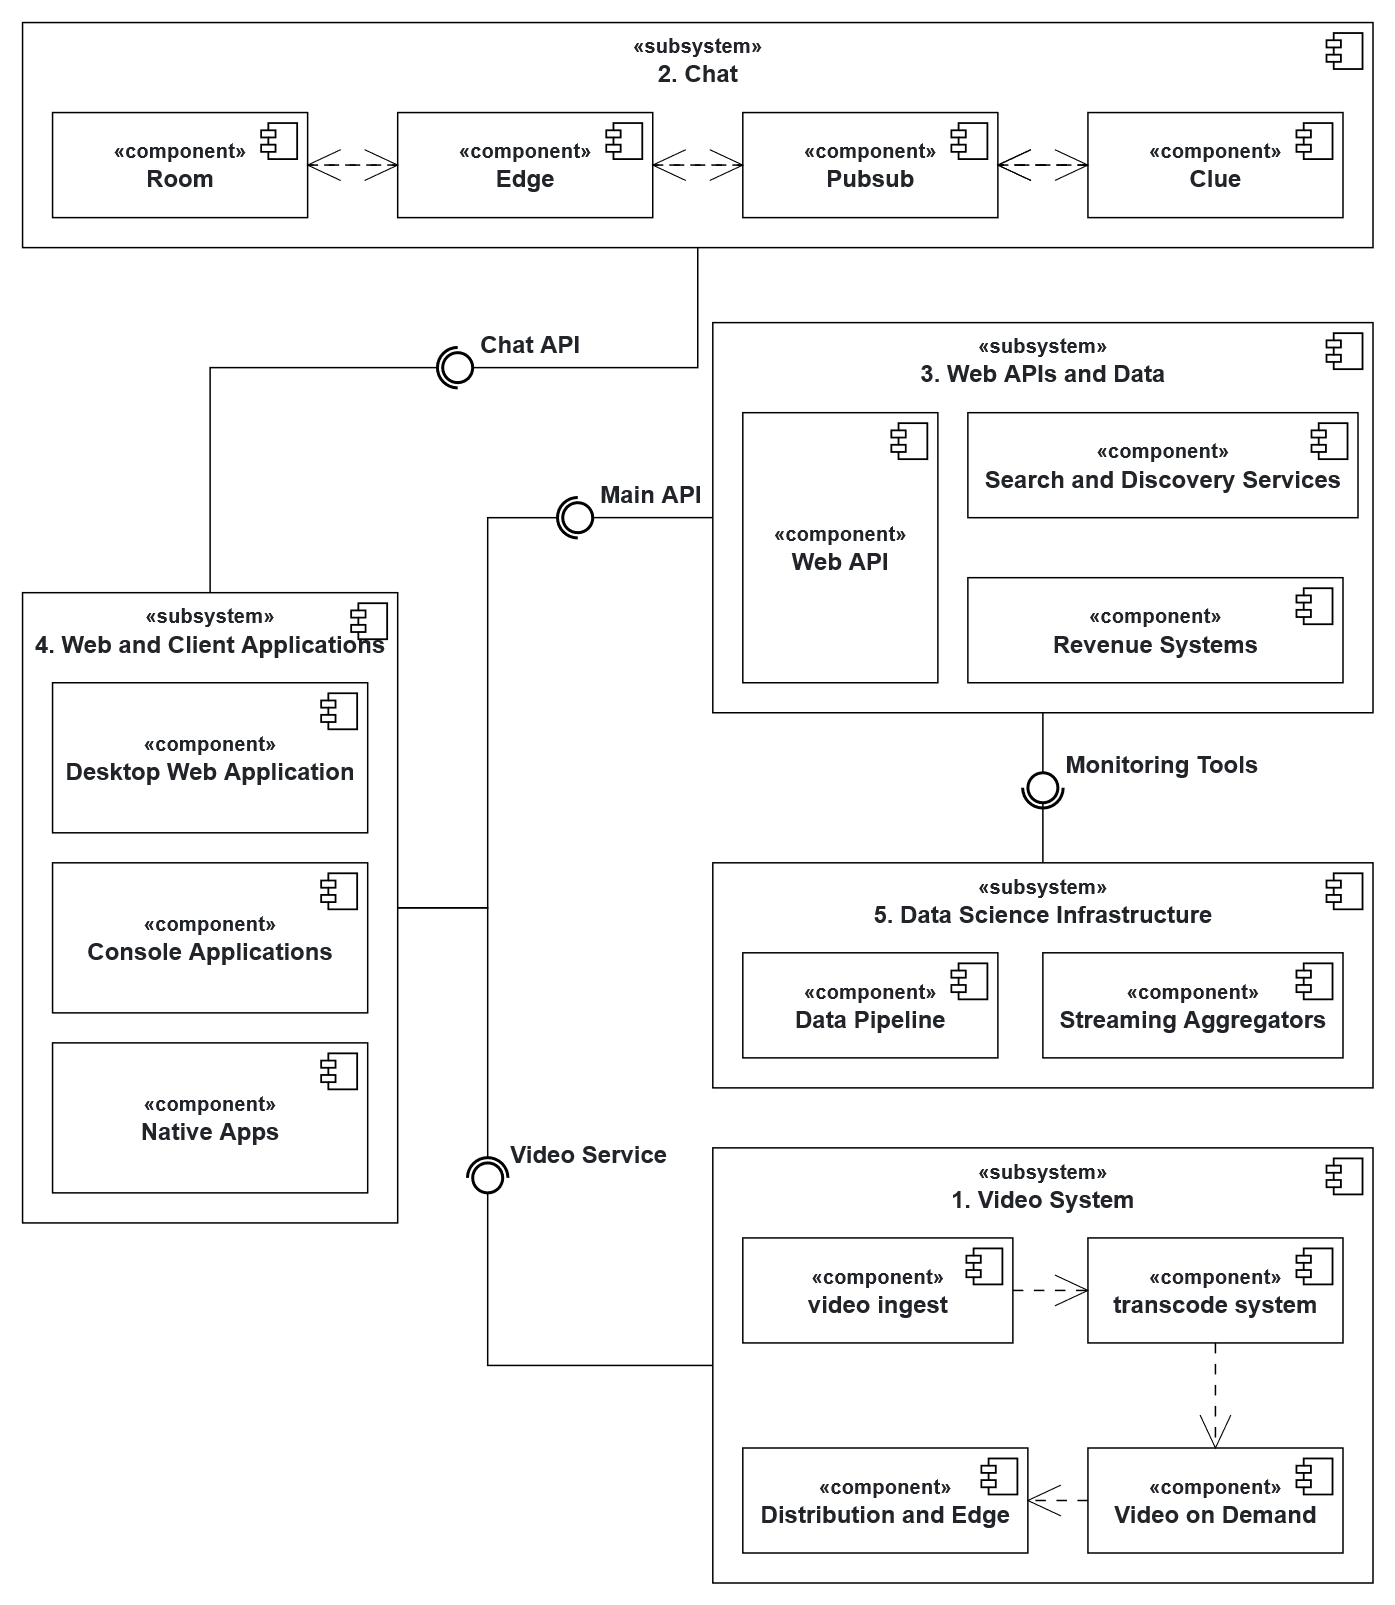
\includegraphics[width=\linewidth]{images/TwitchArchitectureNew.png}
    \caption[System Architecture of Twitch]{System Architecture of Twitch}\label{fig:twitch-architecture}
\end{figure}

\begin{enumerate}
    \item \textbf{Video System}
    
    The video system begins with the \textbf{video ingest} process, where live video streams are received from broadcasters. Twitch primarily uses \ac{RTMP} for this purpose. Once the video stream is ingested, it is transported to the \textbf{transcode system}. This system, implemented in a combination of C/C++ and Go, transcodes the incoming \ac{RTMP} stream into multiple \ac{HLS} streams to allow viewers to switch between different quality streams.
    After transcoding, the streams are distributed through Twitch's global \textbf{Distribution and Edge} network consisting of multiple \ac{POPs}. The \ac{POPs} cache the \ac{HLS} streams and deliver them to users from geographically optimal locations, minimizing latency and buffering. The distribution system, also largely written in Go, is designed to scale massively, ensuring high availability even during peak usage times. Additionally, Twitch archives all live streams through its \textbf{\ac{VOD} system}, making content available for later viewing, either immediately after the live broadcast or as part of a long-term archive~\parencite{twitch_engineering}.
    
    \item \textbf{Chat}

    The chat system is a real-time distributed system, primarily written in Go, and designed to handle real-time interaction between viewers and streamers. The \textbf{Edge} component of the chat system is responsible for receiving and distributing messages between clients and backend services. It supports the \ac{IRC} protocol over both raw TCP and WebSockets, which allows for broad compatibility, including the integration of third-party \ac{IRC} bots.
    
    Next, the \textbf{Pubsub} subsystem is used for the internal distribution of chat messages across various Edge nodes. Together, they create a hierarchical message distribution system capable of executing massive fanout, to guarantee that all users in a chat room receive messages quickly and reliably. The \textbf{Clue} component handles the application of business logic to these chat interactions. For example, it authorizes the user's message by checking if they are banned from a channel, whether they are a subscriber or if they are showing abusive behavior. Clue achieves this by accepting messages forwarded by the Edge nodes and then aggregating data from various databases, internal \ac{API}s, and caches. Using this data, it then evaluates the viewers' messages against existing rules in real-time. Finally, the \textbf{Room} component manages the viewer list for each chat room. It aggregates, stores and queries membership data across all Edge nodes to provide accurate and up-to-date viewer lists, which are crucial for both moderation and user interaction~\parencite{twitch_chat}.

    \item \textbf{Web \ac{API}s and Data}

    Twitch’s platform also includes a set of web \ac{API}s and data services that enable various functionalities, from user profile management to stream discovery. These \textbf{Web \ac{API}s} are built using a combination of Ruby on Rails, Go, and other open-source technologies, designed to handle high request volumes, with Twitch's services processing over 50,000 \ac{API} requests per second on average. These \ac{API}s allow users to manage their profiles, customize subscriptions, and interact with other services on the platform~\parencite{twitch_engineering}.

    Additionally, Twitch also has various microservices for specific use cases such as \textbf{Search and Discovery Services} to help users find streams and content that match their interests or \textbf{Revenue Systems} that manage all aspects of advertising and subscriptions, ensuring that revenue is accurately tracked and distributed to partners~\parencite{twitch_engineering}. 
    
    \item \textbf{Web and Client Applications}
    
    Twitch’s \textbf{Desktop Web Application} began as a vanilla Rails application but has developed into an Ember.js application. For mobile users, Twitch offers \textbf{Native Apps} on iOS and Android platforms as well as \textbf{Console Applications} for major gaming systems, including Xbox One, Xbox 360, and PlayStation 4~\parencite{twitch_engineering}.

    \item \textbf{Data Science Infrastructure}

    Next to its operating infrastructure, Twitch’s data science infrastructure plays an important role in optimizing the platform, improving user experiences, and driving business decisions. At the core of this infrastructure is the \textbf{Data Pipeline}, which is responsible for collecting, cleaning, and loading over a billion events per day into Twitch’s data warehouse~\parencite{twitch_engineering}. 

    The platform also uses so called \textbf{Streaming Aggregators}, which summarize key metrics in near real-time. These aggregators provide broadcasters with immediate feedback on their stream performance, allowing them to make adjustments on the fly to improve viewer engagement~\parencite{twitch_engineering}.

    \item \textbf{Tools and Operational Infrastructure}

    \ac{QA} is critical, with Twitch utilizing both \textbf{Automated Testing Frameworks} such as Jenkins to allow for continuous integration and testing to maintain high code quality across all services.

    In addition to that, there are also several \textbf{Deployment and Rollback Tools}, as well as \textbf{Monitoring and Alerting Systems}, including \href{https://ganglia.info}{Ganglia}\footnote{\url{https://ganglia.info}}, \href{https://graphiteapp.org}{Graphite}\footnote{\url{https://graphiteapp.org}} and \href{https://www.nagios.org}{Nagios}\footnote{\url{https://www.nagios.org}} that monitor the health and performance of the infrastructure, providing real-time alerts and insights that help engineers quickly identify and prevent problems~\parencite{twitch_engineering}.

    Lastly, Twitch’s \textbf{Network Infrastructure} mostly operates on bare-metal \ac{POPs} worldwide while an increasing number of services are being migrated to \ac{AWS}, which helps reduce operational overhead while benefiting from the on-demand scalability and flexibility of cloud services.

\end{enumerate}

\section{Example: Netflix}


\subsection{Overview of Netflix Open Connect}

Netflix Open Connect was developed in 2011 and officially launched in 2012 as a response to the rapidly increasing scale of Netflix's streaming service~\parencite{netflix_functionality}. Before this, Netflix relied on third-party \ac{CDN}s to deliver content to its users. However, as Netflix's share of global internet traffic grew, it became evident that a custom-built \ac{CDN} could provide more efficiency and better performance adapted to Netflix's specific needs.
The core of Netflix Open Connect is its global network of \ac{OCAs}, which are consists of more than 8,000 specialized servers located in over 1,000 locations around the world~\parencite{netflix_open_connect}. These \ac{OCAs} are strategically placed in \ac{ISPs}' data centers and other interconnection points, allowing Netflix to deliver content directly to users without relying heavily on the broader internet infrastructure. 
When a user signs into Netflix or perform other account related actions, the user's client makes a request to the central server(s), which can potentially be far away from the user's current location. However, when a video is requested, the request is sent to one of the nearby \ac{OCAs} which then serves the large video files directly to the user. Hence, this reduces latency and minimizes the amount of internet traffic, as the cached video data only needs to travel from one of the nearby \ac{OCAs} to the user.

\begin{figure}[htpb]
    \centering
    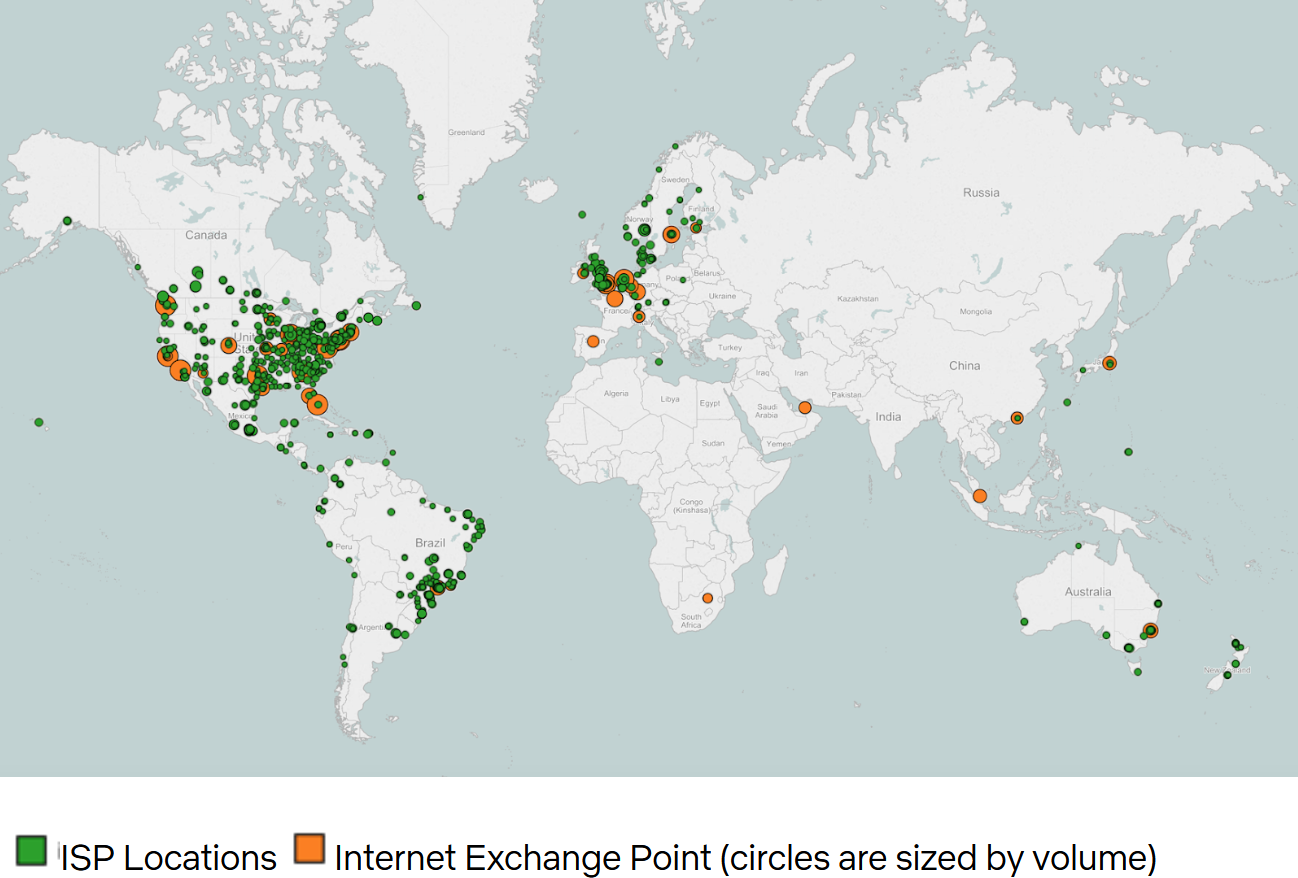
\includegraphics[width=\linewidth]{images/NetflixISP.png}
    \caption[Netflix Open Connect Network as of 2016]{Netflix Open Connect Network as of 2016~\parencite{netflix_open_connect}}\label{fig:netflix-isp}
\end{figure}

\subsection{Content Delivery Mechanism}

Netflix's content delivery strategy involves pre-positioning content on \ac{OCAs} before users request it. This is achieved through advanced algorithms that analyze and predict popular content, to make sure that the most likely to be watched content is already stored close to where it will be consumed~\parencite{netflix_cloud}. For example, in regions with limited internet capacity, such as Australia, Netflix minimizes the use of undersea cables by pre-loading content onto \ac{OCAs} during off-peak hours, reducing the need for real-time content transmission over these expensive and bandwidth-limited connections.

% Netflix also uses consistent hashing to distribute content across multiple servers within a cluster, for balancing workloads and minimizing server churn when the cluster's composition changes~\parencite{netflix_content_distribution}. An example of how this works is the following: Assuming \textit{n} servers, every server ID (\textit{S1} to \textit{Sn}) is hashed 1000 times to generate a reasonably equal distribution of content and also to facilitate fair re-hashing when the cluster changes. Using the uniform consistent hashing approach, then the same weight is assigned to every server.
% For heterogeneous server clusters, which consist of servers with varying storage and throughput capacities, Netflix created a 'Heterogeneous Cluster Allocation' algorithm that allocates content based on both the storage and throughput capacities of individual servers, reducing content holes and improving load balance in clusters that were already heterogeneous~\parencite{netflix_content_distribution}.

\subsection{Performance Optimization and Energy Efficiency}

Over the years, Netflix has continuously optimized its \ac{OCAs}, increasing their efficiency by an order of magnitude since the inception of the program. For instance, the throughput of a single server has been increased from 8 Gbps in 2012 to over 90 Gbps in 2016, largely due to improvements in both hardware and software~\parencite{netflix_open_connect}. These advancements have also led to smaller and more power-efficient \ac{OCAs}.
Additionally, Netflix has optimized its content delivery system to handle high levels of encrypted traffic efficiently. Using hardware acceleration and optimizing memory bandwidth usage, Netflix has reached the capability to serve 100 Gbps\footnote{For FHD (1080p) resolution, which requires a download speed of around 5 Mbps (see \url{https://help.netflix.com/node/306}), 100 Gbps would support 20,000 simultaneous streams.} of encrypted traffic from a single \ac{OCAs}~\parencite{netflix_content_serving}.

\section{Example: YouTube}

YouTube, launched in 2005, is the world's largest video-sharing platform with over 500 hours of video content uploaded every minute, and approximately 694,000 hours of video content streamed per minute~\parencite{youtube_stats}.

\subsection{General Architecture}

YouTube's infrastructure is built on Google's global network of data centers and \ac{CDN}s: The most popular content for a certain region is cached in global \ac{CDN}s that make sure that there are multiple copies of a video to guarantee quality of service, reliability and closeness to the user while the other videos are stored on separate servers in various locations, mainly in the US~\parencite{youtube_architecture_2}. The platform uses advanced video coding formats, such as \href{https://developers.google.com/media/vp9}{VP9}\footnote{VP9 is a video coding format developed by Google and published 2013 to compete with H.265, designed to handle high resolutions up to 65536×65536 pixels and mainly used by YouTube. It works by compressing video content using block-based transformation, where the image is divided into coding units of 64×64 pixels, which are further subdivided into smaller blocks based on the content complexity. A draft of the specification can be found at \url{https://storage.googleapis.com/downloads.webmproject.org/docs/vp9/vp9-bitstream-specification-v0.6-20160331-draft.pdf}} to optimize bandwidth usage while maintaining high video quality, even at lower bitrates~\parencite{youtube_vpu}. 
In recent years, YouTube has also expanded its feature offering to include live streaming and 360-degree videos~\parencite{youtube_live}.

% The following system design model (see \autoref{fig:youtube-system-design}) will not be explained in detail and is meant to help understand and visualize components referenced in this section~\parencite{youtube_architecture}.

% \begin{figure}[htpb]
%     \centering
%     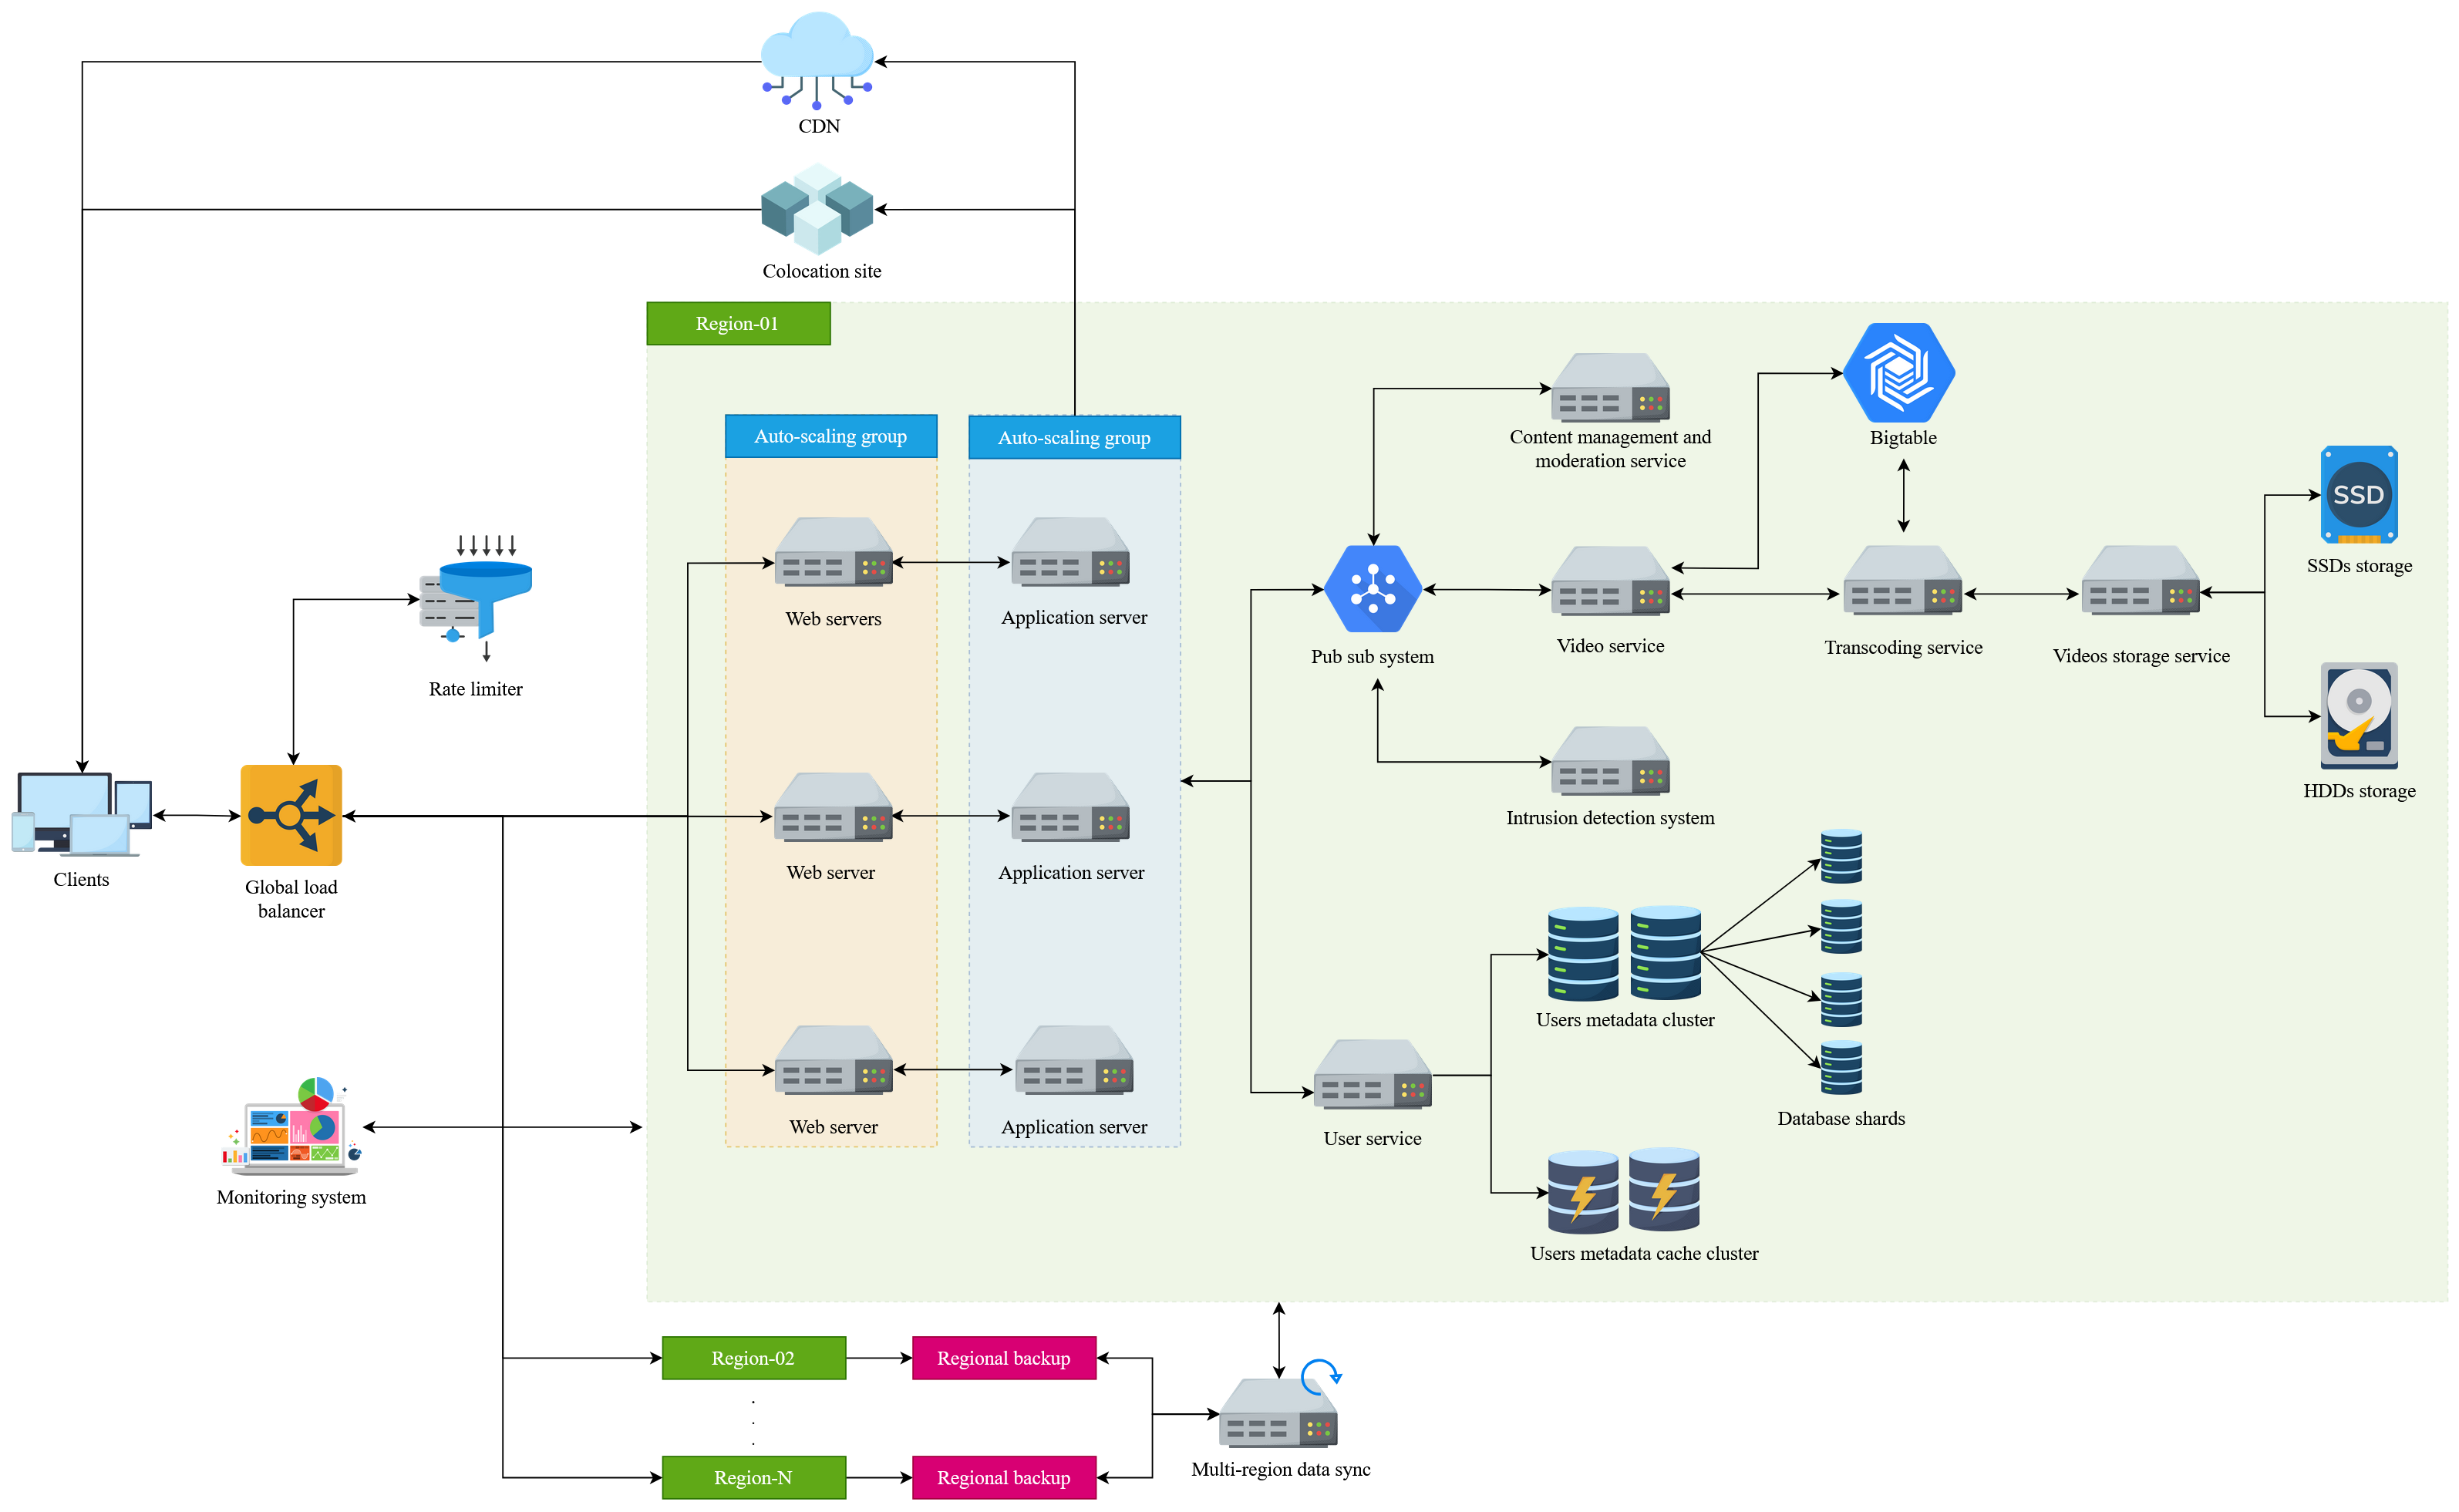
\includegraphics[width=\linewidth]{images/YoutubeSystemDesign.png}
%     \caption[System Architecture of YouTube]{System Architecture of YouTube}\label{fig:youtube-system-design}
% \end{figure}

\subsection{Scalability Challenges}

While there is not much information on current scalability issues published by YouTube, there are several records of problems that the YouTube team faced up to 2012. These challenges included managing rapid and unpredictable user growth with limited resources, as there was not enough budget to maintain excess machines to handle such growth. Additionally, the integration of new features such as social graphs and recommendation algorithms was especially compute-heavy for the platform. The team also pushed the limits of the hardware and software of that time, encountering limitations like performance bottlenecks in database structures before database partitioning (more details in \autoref{section:db-sharding}) ~\parencite{youtube_challenges}. As the platform continued to evolve, identifying these bottlenecks became more difficult, as they often were not due to a issue by YouTube itself, but rather by limitations of other libraries and third party software that they used~\parencite{youtube_challenges_2}.

\subsection{Video Acceleration at Scale}

With Moore's Law slowing down, specialized hardware accelerators optimized for large-scale video transcoding are needed to meet demand for video processing. 
In 2021, the YouTube team presented an accelerator called the \ac{VCU} and showed that by scaling it within Google data centers, it achieved 20-33x improved efficiency\footnote{Measured by performance-per-TCO (total cost of ownership) with 1.0x being the current non-accelerated Skylake system as reference point} compared to the previous well-tuned non-accelerated systems (see \autoref{tab:youtube-vcu})~\parencite{youtube_infrastructure}.

\begin{table}[h!]
\centering
\caption{Throughput and Performance Comparison of Systems~\parencite{youtube_vpu}}\label{tab:youtube-vcu}
\begin{tabular}{|l|cc|cc|}
\hline
\textbf{System}      & \multicolumn{2}{c|}{\textbf{Throughput [Mpix/s]}} & \multicolumn{2}{c|}{\textbf{Perf/TCO}}    \\ \hline
            & \multicolumn{1}{c|}{H.264}       & VP9       & \multicolumn{1}{c|}{H.264} & VP9 \\ \hline
Skylake     & \multicolumn{1}{c|}{714}            & 154           & \multicolumn{1}{c|}{1.0x}      & 1.0x     \\ \hline
4xNvidia T4 & \multicolumn{1}{c|}{2,484}          & --            & \multicolumn{1}{c|}{1.5x}      & --       \\ \hline
8xVCU       & \multicolumn{1}{c|}{5,973}          & 6,122         & \multicolumn{1}{c|}{4.4x}      & \textbf{20.8x}    \\ \hline
20xVCU      & \multicolumn{1}{c|}{14,932}         & 15,306        & \multicolumn{1}{c|}{7.0x}      & \textbf{33.3x}    \\ \hline
\end{tabular}
\end{table}

The core component of the \ac{VCU} system is the encoder core, which serves as a special hardware component acting as an accelerator built for large distributed clusters. 
% It works in three stages: 1. \href{https://en.wikipedia.org/wiki/Macroblock}{\textit{Block-based video encoding}}\footnote{\url{https://en.wikipedia.org/wiki/Macroblock}} (most memory and bandwidth intensive stage), 2. \href{https://en.wikipedia.org/wiki/Entropy_coding}{\textit{entropy encoding}}\footnote{\url{https://en.wikipedia.org/wiki/Entropy_coding}} and 3. \textit{\href{https://www.kernel.org/doc/html/latest/gpu/afbc.html}{loop filtering and lossless frame buffer compression}}\footnote{\url{https://www.kernel.org/doc/html/latest/gpu/afbc.html}}. 
While the \ac{VCU} design optimizes for throughput and system balance, allowing it to adapt to changing workloads and infrastructure demands, its major challenges are handling multiple resolutions and formats and ensuring system reliability in a large-scale environment~\parencite{youtube_vpu}.
Also, the \ac{VCU} integrates multiple encoder cores and a memory system optimized for data center workloads and can be adjusted dynamically depending on the network bandwidth, storage and live/\ac{VOD} demand workloads. This hardware-software co-design approach helps efficiently transcoding uploaded videos while being flexible for future workloads. The system is highly parallelized, allowing for efficient handling of multi-output transcoding where a single input video is processed into multiple resolutions and formats at the same time~\parencite{youtube_vpu}.

The \ac{VCU} system enables otherwise infeasible VP9 compression at scale, caused by VP9's larger block sizes and limited hardware support. This results in new use cases related to live streaming (e.g., using VP9 to encode many short (2-second) segments in parallel to increase overall throughput). \blockquote{\textit{As a concrete example, a 2-second 1080p chunk could be encoded in 10 seconds, the encoding system would transcode 5-6 chunks concurrently to achieve the needed throughput of a 1 video-sec/second}}~\parencite{youtube_vpu}.
Currently, this system is mainly used by YouTube for a wide range of video workloads, including video sharing, live streaming and cloud gaming. 
% !TeX root = ../main.tex
% !TeX root = ../main.tex
% Add the above to each chapter to make compiling the PDF easier in some editors.

\chapter{Fundamentals of TUM-Live}\label{chapter:fundamentals}

\section{GoCast Lecture Streaming Service}

\subsection{Overview}
GoCast is a fully self-hosted platform for live streaming and recording of lectures developed by students at \ac{TUM}. The source code is open-source, accessible at \href{https://github.com/TUM-Dev/gocast}{github.com/TUM-Dev/gocast} and licensed under the MIT license. Its main features include:

\begin{itemize}
    \item Automatic live streaming from auditoriums based on lecture schedules imported from CAMPUSonline (campus management system used at \ac{TUM} as TUMOnline).
    \item Self-service interface for lecturers to schedule and manage their \ac{VOD}s and streams.
    \item Automated import of lecture schedules and enrollments from CAMPUSonline.
    \item Self-streaming via third party streaming software such as \href{https://obsproject.com}{OBS}\footnote{\url{https://obsproject.com}}, \href{https://zoom.us}{Zoom}\footnote{\url{https://zoom.us}}, etc.
    \item Automatic recording of live streams.
    \item Manual \ac{VOD} uploads.
    \item Automatic post-processing of recordings.
    \begin{itemize}
        \item Detect silence in videos and makes them skip-able.
        \item Transcribe live streams and \ac{VOD}s using the \href{https://github.com/openai/whisper}{Whisper LLM}\footnote{\url{https://github.com/openai/whisper}}.
        \item Generate thumbnails.
    \end{itemize}
    \item Optional live chat for viewers to ask questions.
    \begin{itemize}
        \item Polls can be created by lecturers.
        \item Questions can be upvoted by viewers and answered or hidden by lecturers.
        \item Optional moderation features for lecturers.
    \end{itemize}
\end{itemize}

\subsection{Current System Architecture}

\begin{figure}[htpb]
    \centering
    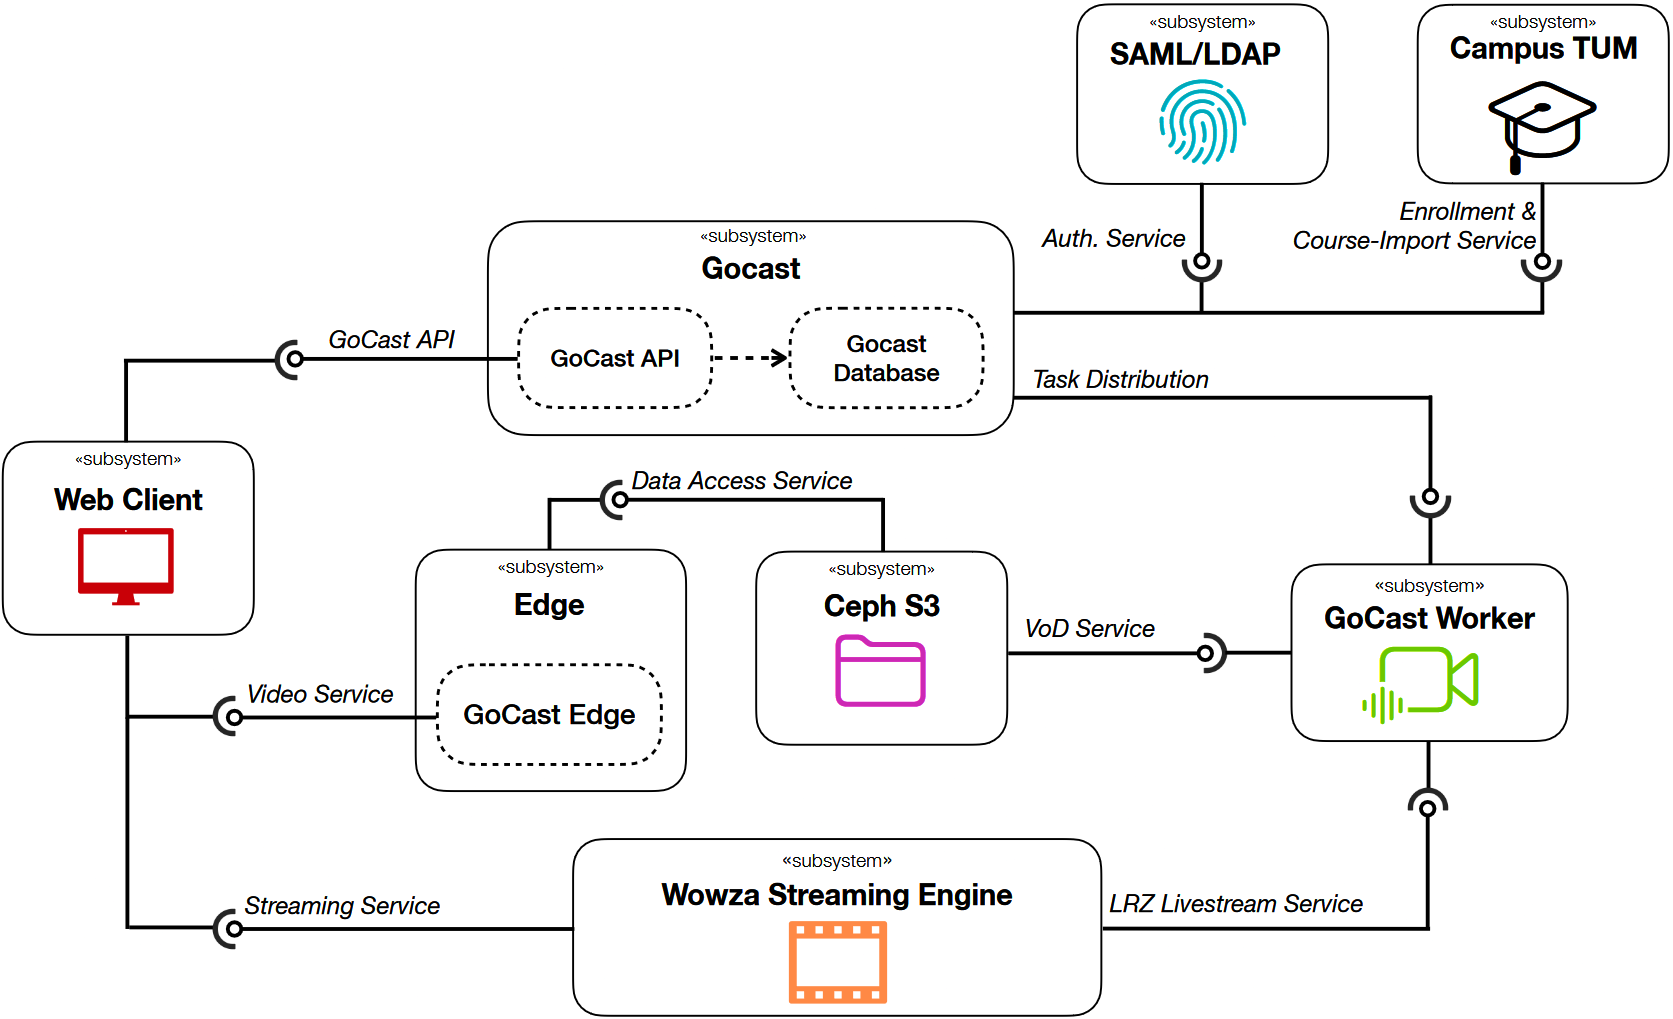
\includegraphics[width=\linewidth]{images/ssd-new.png}
    \caption[System Architecture of GoCast]{System Architecture of GoCast}\label{fig:old-system-architecture}
\end{figure}

The current system architecture of GoCast can be divided into three parts:

\subsubsection{1. User-, course- and task-management:}
At the core of the GoCast system, there is the main \ac{API} built on the \href{https://github.com/gin-gonic/gin}{Gin-Gonic}\footnote{\url{https://github.com/gin-gonic}} Framework and connected to a \href{https://mariadb.org}{MariaDB}\footnote{\url{https://mariadb.org}} Database. Its main functionality is to manage users, courses, streams, pull events from CAMPUSonline and schedule tasks. For user authentication, it can use \ac{SSO} and \ac{SAML} to allow users to authenticate themselves with their university credentials.

\subsubsection{2. \ac{VOD} upload related components:}
Next, whenever a lecture is uploaded as a VOD, the video data is sent to a Worker which then transcodes and segments the video into MPEG-2 compressed video transport stream files using \href{https://ffmpeg.org/}{FFmpeg}\footnote{\url{https://ffmpeg.org}}. These segments are then copied to a shared storage using the VOD Service component so that they can then later be distributed by the Edge Server to the end-user.
Currently there are plans to replace the Worker subsystem with a more robust and efficient Runner system. However, as the Runner is still in the development phase and not tested yet (see \autoref{subsection:runner}), we will mainly refer to the Worker subsystem throughout this thesis (although in principle the Worker and Runner concepts can be used interchangeably).

\subsubsection{3. Lecture recording and live streaming:}
Lastly, for live streaming GoCast depends on external streaming infrastructure. In \ac{TUM}'s case this is the live streaming infrastructure of the \ac{LRZ} which internally runs the \href{https://doku.lrz.de/allgemeines-526418642.html}{Wowza Streaming Engine}\footnote{\url{https://doku.lrz.de/allgemeines-526418642.html}}. Whenever a lecturer starts a live stream from a lecture hall, the produced \ac{RTMP} stream is sent via the Worker to the \ac{LRZ} streaming service which then processes the live stream and makes it available for the viewer in real-time. When the viewer now watches a live stream, the video is streamed directly to the user's browser client from the \ac{LRZ} streaming service. 

\section{TUM-Live}\label{section:tum-live-history}

GoCast is in use at the \ac{TUM} as \href{https://tum.live}{TUM-Live}. This section aims to group and structure existing information related to TUM-Live's history, technical setup and statistics in a concise manner. 

\subsection{Technical Setup of TUM-Live}

To professionally stream hundreds of lectures every semester, TUM-Live has integrated GoCast in a complex infrastructure of hardware components deployed in separated VLANs that allow for easy streaming from a lecture hall without having to do additional configuration at the beginning of each lecture. 
First, there needs to be at least one pan–tilt–zoom camera equipped in a lecture hall to record and follow the lecturer as well as the white-/blackboard.
Then, every lecture hall needs to be equipped with a so called \href{https://www.extron.com/article/smp}{\ac{SMP}}\footnote{\url{https://www.extron.com/article/smp}} which is an all-in-one recording and streaming processor that captures, switches, scales and distributes audio and video sources and presentations. In addition to that, it also provides multiple concurrent streams including flexible two-window layouts and full screen views. This is especially useful as it allows sending video data in three different formats to the main TUM-Live instance: \texttt{CAM} for the camera pointing at the lecturer, \texttt{PRES} for the currently shown screen of the lecturer's laptop or \texttt{COMB} for a two-window view of both. The \ac{SMP} can also be used as a backup device for the \ac{VOD} in case something goes wrong in a later stage (e.g., a Worker has an outage and the recorded stream is "lost") as the \ac{SMP} device creates a local copy of the recording. The main problem with \ac{SMP}s is their high cost, as one device can cost more than 10,000 EUR.

\subsection{Progress of TUM-Live}

Originally, TUM-Live was started in 2019 by the multimedia group of the former faculty of informatics to stream overcrowded lectures of popular courses into different lecture halls as some courses had more students than lecture hall seats. A lecturer would create a RTMP stream of his current lecture and publish the stream in a private network to a different lecture hall which then would display the streams to the students. At the same time this system started being used more and more to provide a public live stream and \ac{VOD} portal and archive for students of selected courses. The system itself was - in comparison to the current system - rather simple as it displayed a list of streams\footnote{\url{https://web.archive.org/web/20191001114650/https://live.rbg.tum.de}} that would show the currently live stream or link to uploaded .mp4 files.
This quickly changed in 2020 as the COVID-19 pandemic created a high demand for online lecture video streams, which then resulted in the development of GoCast. Starting from fall 2021, the old TUM-Live system switched to using GoCast, as provided a user friendly and easily accessible user interface for students and a cost-efficient and privacy-focused alternative to other lecture streaming platforms for \ac{TUM}'s media group "ProLehre". 

Nowadays, TUM-Live offers live and on-demand videos of lectures and events from \ac{TUM}'s \href{https://www.cit.tum.de}{\ac{CIT}}\footnote{\url{https://www.cit.tum.de}}. Some of \ac{TUM}'s other schools have also shown interest in joining the \ac{CIT} in using TUM-Live, but do not have the budget to equip all lecture halls with \ac{SMP}s. However, this issue might soon be resolved, as a student has developed his own open-source \ac{SMP} called \ac{VMP} that aims to re-implement the functionality of the \ac{SMP} in software, using the \href{https://gstreamer.freedesktop.org/}{GStreamer Multimedia Framework}\footnote{\url{https://gstreamer.freedesktop.org/}}. The target hardware is a small single-board computer with accelerated Multimedia encoding/decoding and additional HDMI capture capabilities which costs only around 500 EUR. Given the low cost of such a device, it is very likely that other \ac{TUM} schools and possible even other universities will join TUM-Live in the future.

\subsection{User Statistics of TUM-Live}\label{subsection:user-stats-tumlive}

Since its creation in February 2021, TUM-Live has been used to stream thousands of hours of video every semester for more than 1,300 courses, 20,000 streams and 30,000 students. The following plots (see \autoref{fig:tumlive-stats}) display a broad overview of viewer metrics from the current system. As the \textit{VoD activity throughout the day} plot shows, the hours at which the users watch recorded \ac{VOD}s is normally distributed, with the mean being around 4PM. Most students use TUM-Live throughout the entire lecture week (see \textit{VoD activity per day of week} plot showing an evenly distributed \ac{VOD} activity over the week), meaning that the Edge Servers need to be fully functional at all times. At its peak, there are nearly 6,000 \ac{VOD} replays per day (see \textit{VoD activity per day}) while at times - mostly during the semester breaks - there are weeks with nearly no \ac{VOD} activity at all.

\begin{figure}[htpb]
    \centering
    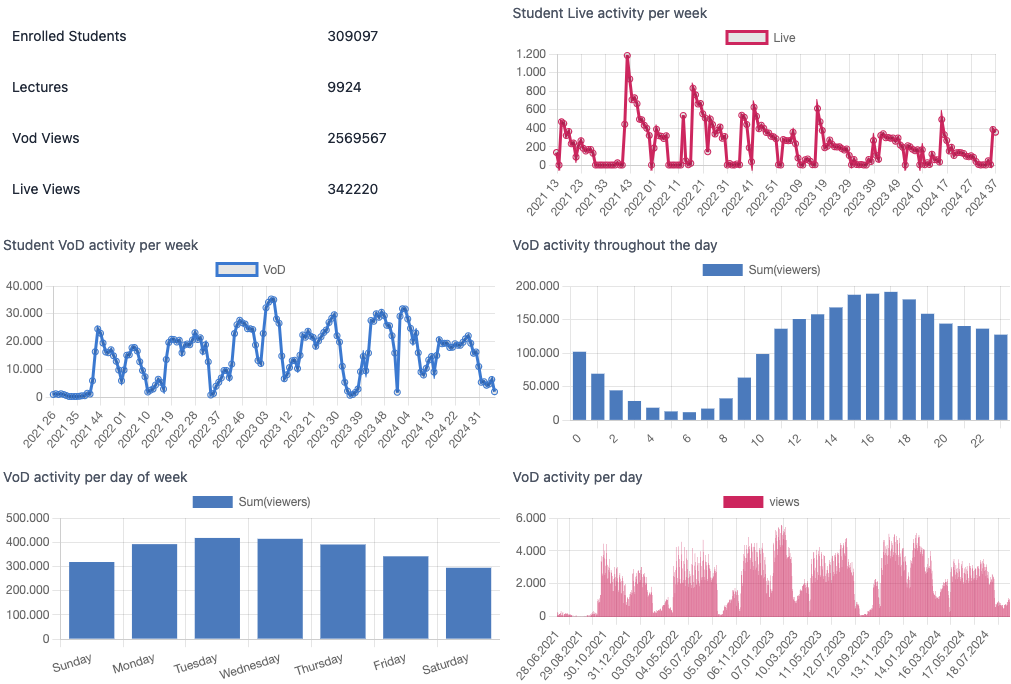
\includegraphics[width=\linewidth]{images/TUMLiveStats.png}
    \caption[TUM-Live Statistics]{TUM-Live Viewing Statistics}\label{fig:tumlive-stats}
\end{figure}

What's especially interesting is the development of the number of users, courses and streams over time. As can be seen in \autoref{fig:tumlive-stats-2}, at the beginning of each semester there is a clear spike in new users, created courses and streams. This is mainly due to the automatic import of lecture data and enrollments from CAMPUSonline. Between semesters, the increase in new users and courses is rather flat, with a slight increase in the number of streams (mostly streams that have been created manually).  

\begin{figure}[htpb]
    \centering
    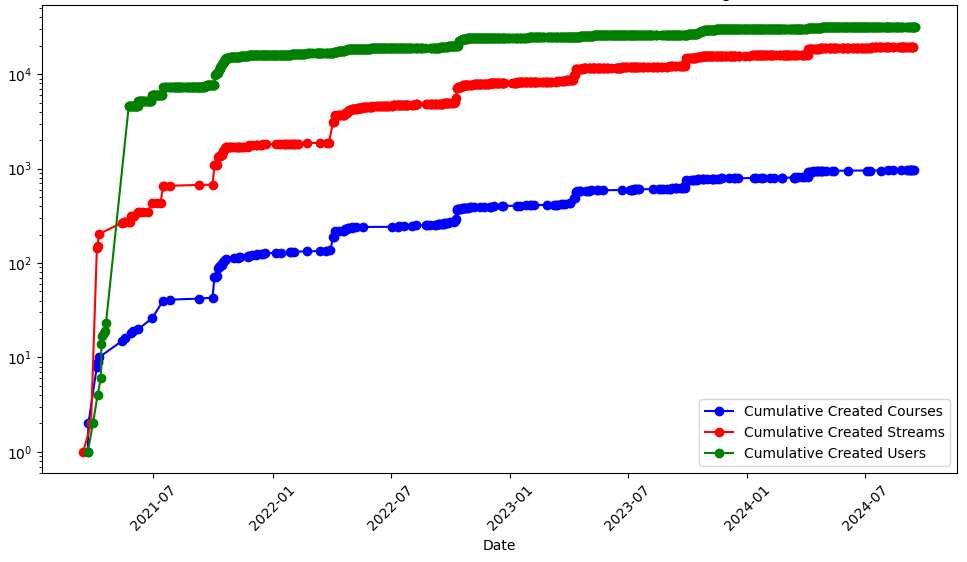
\includegraphics[width=\linewidth]{images/TUMLiveStats2.png}
    \caption[Cumulative Number of Users, Courses and Streams over Time (Log Scale)]{Cumulative Number of Users, Courses and Streams over Time (Log Scale)}\label{fig:tumlive-stats-2}
\end{figure}

% !TeX root = ../main.tex
\chapter{Scaling Video Streaming Architecture}\label{chapter:videostreaming}

This chapter focuses on how video streaming actually works, what processes are involved in designing and deploying the infrastructure of a video streaming service and what its potentials and challenges in regards to scalability and performance are.   

\section{Video Streaming}

In the following section, the most important technical concepts of video streaming are explained and compared.

\subsection{Video Streaming Types}
The concept of video streaming was already present during the early years of television. However, nowadays video streaming is mostly used to describe transmitting videos over the Internet. In the following are described the most important types of video streaming with their specific technical requirements and challenges:

\begin{itemize}
    \item \textbf{Live Streaming:} This type involves real-time broadcasting of video content, often used for events, gaming and news. As already mentioned in the overview of Twitch's architecture, live streaming requires a robust architecture capable of handling high concurrency and maintaining low latency. Technologies such as \ac{RTMP} and \ac{HLS} are commonly used. Ingest servers then process incoming streams from broadcasters, encode them in multiple bitrates, and distribute them through \ac{CDN}s to ensure smooth delivery to viewers.
    \item \textbf{Video on Demand:} \ac{VOD} services (such as YouTube, Netflix, etc.) allow users to select and watch video content at any time. This type of streaming relies heavily on efficient storage systems and \ac{CDN} to manage large content libraries and ensure quick access. \ac{VOD} systems often use progressive streaming techniques, where large video files are segmented and is streamed in small chunks as the user watches the video, allowing for a more efficient viewing experience without requiring the entire video to be downloaded upfront~\parencite{cloud_streaming_trends}.
    \item \textbf{Webcasting:} Webcasting is similar to live streaming but typically used for structured events like corporate meetings, webinars, and online training (e.g., via Zoom, BBB or Teams). It often involves additional features such as viewer authentication, interaction capabilities, and detailed analytics. The architecture must support both high scalability and customization for enterprise-level use~\parencite{cloud_streaming_trends}.
    \item \textbf{On-Demand Streaming:} A subset of \ac{VOD}, where content is streamed as it is requested by users without pre-buffering. This type of streaming requires efficient backend systems to handle large numbers of concurrent requests while minimizing latency~\parencite{cloud_streaming}.
    % \item \textbf{Progressive Download:} In this method, video content is downloaded in segments and begins playback as soon as enough data has been buffered. This approach is useful in scenarios with fluctuating network conditions, as it allows the video to play without interruption~\parencite{progressive_download}.
    \item \textbf{Peer-to-Peer Streaming:} In \ac{P2P} streaming, viewers share the content they are streaming with others, reducing the load on central servers and enhancing bandwidth efficiency. \ac{P2P} streaming can be challenging to manage due to the need for sophisticated algorithms to optimize peer selection, data distribution, and to ensure low latency and high reliability across the network~\parencite{p2p}. This type of streaming is often used by sports or news broadcasters.
\end{itemize}

\subsection{Video Transcoding}
Once a video has been recorded, it needs to be transcoded into different formats to ensure compatibility across various devices and platforms while maintaining as much of its original quality as possible. The process can be broken down into five operations:

\begin{itemize}
    \item \textbf{Standard Transcoding} involves changing video compression standard of the video, e.g., by switching between different codecs such as H.265/HEVC or H.262/MPEG-2 to support different devices. It is important to note that when changing codec, it has to decode the bitstream with the old codec first and then encode it again with the new codec, making the entire operation very compute-intensive.~\parencite{codec_transcoding}.
    \item \textbf{Bitrate Transcoding/Transrating} adjusts the bitrate of a video stream to balance the quality of the video and subsequent bandwidth usage. For instance, a high-resolution video may need to be transcoded to a lower bitrate for users with limited bandwidth. \ac{ABR} is often used for this, as multiple bitrate streams are generated, leaving the decision of which frame rate to select up to the client based on current network conditions~\parencite{transcoding}.
    \item \textbf{Spatial Transcoding/Transsizing} modifies the resolution of a video to match the capabilities of the viewing device. For example, a 4K video may be downscaled to 1080p or 720p for playback on devices that do not support higher resolutions~\parencite{cloud_streaming}.
    \item \textbf{Frame Rate Transcoding} modifies the number of frames in a video file - usually by reducing the number of frames by removing frames in a certain distance so that the human visual system doesn't notice a difference~\parencite{transcoding}.
    \item While Transcoding changes the contents of the file, converting the video file format (e.g., from .avi to .mp4), is often referred to as \textbf{Format Transcoding/Transmuxing} as it changes the container and not the actual content. This step often includes re-encoding audio streams to formats like AAC or Opus, depending on the target platform~\parencite{transcoding}.
\end{itemize}

Also, it needs to be mentioned that there are different compression techniques used as part of the transcoding process, with the two primary methods being:

\begin{itemize}
    \item \textbf{Lossy Compression:} This technique reduces file size by removing some of the video data, which can affect quality but significantly decreases bandwidth usage. Popular lossy codecs include H.264, H.265, and VP9~\parencite{combression}.
    \item \textbf{Lossless Compression:} On the other hand, lossless compression reduces file size without any loss of data, preserving the original quality. However, the compression ratios are typically much lower compared to lossy methods. Codecs like Apple ProRes and FFV1 are examples of lossless compression used in professional environments~\parencite{combression}.
\end{itemize}

\subsection{Delivery Networks}
Delivery networks ensure that video content reaches end-users quickly and reliably. The two main approaches for this are \ac{CDN}s and \ac{P2P} networks:

\ac{CDN}s are a network of geographically distributed servers that cache video content close to end-users. When a user requests content, the request is routed to the nearest \ac{CDN} node, which delivers the content with minimal latency. \ac{CDN}s like Amazon CloudFront, Azure CDN, and Google Cloud CDN are designed to handle massive amounts of traffic and can scale dynamically based on demand~\parencite{cdn_basic}.
Technically, \ac{CDN}s work by replicating video content across multiple nodes in different locations. Each node (or edge server) holds a copy of the content, reducing the distance data must travel and therefore improving load times and reducing latency. Advanced \ac{CDN}s also use techniques such as Anycast routing, where a single IP address is shared by multiple servers, and requests are automatically routed to the nearest or least-loaded server~\parencite{cdn_basic}.
    
As mentioned before, \ac{P2P} streaming takes advantage of the bandwidth of viewers to distribute content. Instead of relying on a central server, each user in the network shares parts of the video stream with others. This method reduces the load on central servers and can improve scalability, especially for live streaming with high concurrency~\parencite{cdn_basic}.
However, \ac{P2P} networks require complex algorithms to ensure optimal peer selection and data distribution. Algorithms like BitTorrent's Tit-for-Tat, which motivate users to share data by rewarding them with faster downloads, are often used for this. Additionally, latency in \ac{P2P} networks is managed through buffer management strategies and protocols designed to minimize the delay in data exchange between peers~\parencite{p2p}.

\subsection{Security}

Most video streaming services handle licensed data such as movies or copyrighted music and need to guarantee that its content is protected from unauthorized access, piracy, and other malicious activities.
There are three factors that need to be considered when evaluating the security of a streaming service: 

First, ensuring that only authorized users can access certain content. This is most often achieved through various methods, including \ac{JWT} based authentication, which generates a unique \ac{JWT} for each session, or protocols such as OAuth. What's important is, that the authentication and access control is strictly applied on all levels - not just when a user accesses the streaming service, but also on an individual request basis to avoid that an authorized user can access forbidden scopes. A relevant example for this is streaming services that require authentication for a user to access the platform, but then don't require any authentication for accessing specific content. A malicious user could use this to, for example, download full videos by checking the source URL of the video and simply accessing the full video from there. Alternatively, there are also other attack vectors such as possible file and directory discovery where "\textit{adversaries may enumerate files and directories or may search in specific locations of a host or network share for certain information within a file system}"~\parencite{mitre}. A simple solution to defend from this kind of access would be to ensure that all content can only be accessed with a valid \ac{JWT} (or any other form of token) that is limited with regards to the scope and validity.

Secondly, to prevent piracy, or any unwanted activities, one can use \ac{DRM} tools like Microsoft's PlayReady, Apple's FairPlay, and Google's Widevine protect content by controlling how it is accessed and used. \ac{DRM} typically involves encrypting the content and then using licenses to grant authorized users the ability to decrypt and play the content. The encryption process usually involves \ac{AES} with 128-bit or 256-bit keys. When a user attempts to play \ac{DRM}-protected content, the video player requests a license from a \ac{DRM} server. If the user is authorized, the server provides the license, which includes the decryption key. The player then decrypts the content and plays it~\parencite{drm}. However, as many of these \ac{DRM} services require a paid license, one needs to consider if it is worth the additional effort and expense.

Lastly, protecting the infrastructure itself is critical. Beyond DRM, video streams are often encrypted during transmission (e.g., using \ac{TLS})to protect against interception. Techniques such as IP whitelisting, port restriction, and the use of firewalls are standard practices. Additionally, regular security audits and real-time monitoring can help identify and mitigate potential threats.

% \section{Deployment}
% Efficient deployment strategies are essential for scaling video streaming services to meet user demands while maintaining performance and reliability. Depending on the size and extent of the project, one approach might be better than another and help save significant time when developing and deploying the different microservices of a streaming service (more on that in \autoref{chapter:scaling_tumlive}). This section is meant to give an overview of the most popular deployment technologies and discuss their functionality, use cases and monitoring tools.

% \subsection{Docker}
% TODO
% Docker is a containerization platform that allows developers to package applications and their dependencies into containers. These containers can then be deployed consistently across various environments, ensuring that the application behaves the same way regardless of where it runs.

% In video streaming, Docker is used to encapsulate encoding services, web servers, databases, and other components. Containers can be easily scaled across multiple servers, enabling the deployment of video streaming applications in a distributed and scalable manner. Docker images can be versioned and deployed through Continuous Integration/Continuous Deployment (CI/CD) pipelines, allowing for rapid updates and rollbacks without downtime~\parencite{docker_deployment}.

% \subsection{Docker Swarm}
% TODO
% Docker Swarm extends Docker's capabilities by enabling clustering and orchestration of containers across multiple hosts. It allows for the seamless management of a large number of containers, automatically distributing workloads across a cluster to optimize resource utilization.

% In the context of video streaming, Docker Swarm can be used to manage the various microservices involved in streaming, such as encoding, storage, and delivery. Swarm handles tasks like load balancing, scaling containers up or down based on demand, and ensuring high availability by replicating services across different nodes~\parencite{docker_swarm_deployment}.

% \subsection{Kubernetes}
% TODO
% Kubernetes is an advanced orchestration platform that automates the deployment, scaling, and management of containerized applications. Kubernetes offers more advanced features than Docker Swarm, including automatic scaling, self-healing, and rolling updates.

% For video streaming services, Kubernetes can manage thousands of containers across a distributed infrastructure. It ensures that services remain available even if some nodes fail, by automatically rescheduling containers on healthy nodes. Kubernetes' Horizontal Pod Autoscaler can dynamically adjust the number of running containers based on CPU utilization or custom metrics, ensuring that the streaming service can handle fluctuating demand~\parencite{kubernetes_video_deployment}.

% Kubernetes also supports StatefulSets, which are essential for managing stateful applications like databases, ensuring that each instance maintains its identity across reschedules. This is particularly important for maintaining the consistency and availability of data in video streaming platforms~\parencite{statefulset_kubernetes}.

% \subsection{Monitoring Tools}
% To keep an overview of what the current status of the system is and analyze past errors and logs, monitoring is essential. Several (open source) tools are commonly used in the industry:

% \begin{itemize}
%     \item \textbf{Network Performance} tools like \href{https://github.com/NagiosEnterprises/nagioscore}{Nagios} and \href{https://github.com/zabbix/zabbix}{Zabbix} monitor and analyze network traffic, server health and bandwidth to identify bottlenecks and optimize network performance.
    
%     \item \textbf{CDN Monitoring} tools such as \href{https://github.com/DataDog/datadog-agent}{Datadog} track \ac{CDN} performance, latency, and availability, ensuring that content delivery is optimized across different geographic regions.
    
%     \item \textbf{Video Quality Monitoring} tools like \href{https://github.com/ccrisan/streameye}{StreamEye} or \href{https://github.com/Netflix/vmaf}{VMAF (Video Multimethod Assessment Fusion)} assess video quality from the viewer's perspective. These tools analyze factors like resolution, bitrate, and compression artifacts to ensure that the delivered video meets quality standards.
    
%     \item \textbf{Error Tracking} systems like \href{https://github.com/getsentry/sentry}{Sentry}, \href{https://github.com/rollbar?q=&type=all&language=&sort=stargazers}{Rollbar}, and \href{https://github.com/grafana/grafana}{Grafana} detect and report errors in real-time, allowing for rapid response to issues that could affect the streaming experience.
    
%     \item \textbf{Logging and Dashboards} tools like \href{https://github.com/grafana/loki}{Loki}, \href{https://github.com/prometheus/prometheus}{Prometheus}, and \href{https://github.com/grafana/grafana}{Grafana} provide detailed insights into system performance, user behavior, and potential issues. These tools can be integrated into real-time dashboards and connected to third party notification services, offering a clear overview of the entire streaming infrastructure and instant alerts to allow for immediate countermeasures.
% \end{itemize}

\section{Cloud-Based Video Streaming}

In 2008 Netflix started to migrate all its services to the cloud (\ac{AWS}) to move away from vertically scaled single points of failure, like relational databases, towards highly reliable, horizontally scalable, distributed systems in the cloud~\parencite{netflix_aws}. Since then it has become the standard to deploy and scale using third party cloud services. This section goes into detail how this can be especially useful for video streaming infrastructure. 

\subsection{Architecture}
Cloud-based video streaming architecture typically involves multiple layers, each responsible for different aspects of the streaming process:

\begin{itemize}
    \item \textbf{Content Storage:} Platforms like Amazon S3, Azure Blob Storage, and Google Cloud Storage offer scalable and reliable storage solutions for video content. These platforms use object storage systems designed to handle massive amounts of unstructured data. Data is often stored in multiple copies across different geographic locations to ensure durability and availability~\parencite{cloud_streaming}. (see also \autoref{tab:comparison_storage_delivery})
    
    \item \textbf{Encoding and Transcoding:} Cloud services like AWS Elemental MediaConvert, Azure Media Services, and Google Cloud Video Intelligence handle the encoding and transcoding of video into various formats and bitrates. These services are designed to scale automatically based on the volume of content being processed, ensuring that even large video libraries can be encoded efficiently~\parencite{cloud_streaming}.
    
    \item \textbf{Content Delivery Networks (CDNs):} As mentioned earlier, cloud-based \ac{CDN}s such as Amazon CloudFront, Azure CDN, and Google Cloud CDN are essential for delivering video content globally.~\parencite{cloud_streaming}.
    
    \item \textbf{\ac{API}s and Microservices:} Cloud-based architectures often rely on microservices, each responsible for a specific function, such as user authentication, recommendation engines, and analytics. These microservices communicate through \ac{API}s, which can be easily deployed, scaled and updated independently using systems cloud engines such as Azure Kubernetes Service or Google Kubernetes Engine~\parencite{cloud_streaming}.
\end{itemize}

\subsection{Comparison: In-house Storage vs. Cloud Storage}

When designing the architecture of a video streaming service, an important decision is to decide how and where the actual video data should be stored. The following table (\autoref{tab:comparison_storage_delivery}) and subsection summarize the key characteristics of these three approaches in the context of video streaming. 

\textbf{In-House Storage} involves managing own physical storage infrastructure. This allows the owner full control over how the data is managed and allows also for highly customizable configurations, which can be a hard requirement for organizations bound to strict compliance regulations. However, it demands significant upfront capital expenditure and ongoing maintenance. Also, its scalability is limited by the physical infrastructure, requiring careful capacity planning and potentially costly upgrades making short-term adjustments to handle flexible loads very difficult. 

\textbf{Cloud Storage}, on the other hand, offers a flexible and scalable solution managed by third-party providers like AWS, Google Cloud, or Microsoft Azure. It allows video streaming providers to scale their storage needs dynamically without significant upfront investment or configuration effort, as most use cases are already covered by default configurations and extensive documentation and support if necessary. However, while often operating on a pay-as-you-go model, it comes at the cost of limited control over data and potential security concerns that are dependent on the cloud provider's policies. Cloud storage also introduces variability in latency depending on the location of data centers relative to users, and while it is cost-effective in the short term, long-term costs and migration issues due to vendor lock-in can accumulate as data usage grows \parencite{cloud_streaming_cost}.

While not exactly being an alternative storage method, \textbf{\ac{P2P}} systems are highly scalable and can be a very cost-effective way to distribute and store data. However, they come with challenges related to security, data integrity, and performance consistency, as they rely on the cooperation of peers~\parencite{p2p}. Latency and quality of service can vary significantly depending on network conditions and peer availability, making \ac{P2P} suitable for environments where cost savings are prioritized, and some variability in performance is acceptable.

\begin{table}[h]
    \centering
    \caption{Comparison of In-House Storage, Cloud Storage, and P2P for Video Streaming}
    \label{tab:comparison_storage_delivery}
    \resizebox{\linewidth}{!}{%
        \begin{tabular}{|l|c|c|c|}
            \hline
            \textbf{Factor} & \textbf{In-House Storage} & \textbf{Cloud Storage} & \textbf{P2P} \\ \hline
            \textbf{Control} & Full & Limited & Distributed \\ \hline
            \textbf{Security} & High, customizable & Provider-dependent & Lower, peer-based \\ \hline
            \textbf{Scalability} & Hardware-dependent & Virtually unlimited & Highly scalable \\ \hline
            \textbf{Costs} & High upfront, low ongoing & Pay-as-you-go & Low infrastructure cost \\ \hline
            \textbf{Performance} & Low latency & Variable & Variable \\ \hline
            \textbf{Management} & High maintenance & Low maintenance & Complex, peer-managed \\ \hline
            \textbf{Redundancy} & Customizable, local & High, managed by provider & Peer-based, variable \\ \hline
            \textbf{Compliance} & Easier to customize & Provider-dependent & Difficult to enforce \\ \hline
            \textbf{Latency} & Low & Moderate to high & Variable \\ \hline
            \textbf{Use Case} & Enterprise & Scalable, flexible & Cost-sensitive, user-driven \\ \hline
        \end{tabular}
    }
\end{table}

\section{Database Sharding}
While the previous sections described general concepts of streaming, this section is meant to focus on a more specific problem that video streaming services face when scaling up. 
With an increasing number of uploaded videos, there is the issue of running out of storage space. This can easily be solved be buying either a larger storage system or by extending the current storage system with cluster of storage systems. However, when running out of space in a relational database, the options are more limited. One can still upscale the current database, but for large amounts of data - especially for services such as YouTube or Netflix - a single database is not enough. Adding additional databases can however be a complex task, especially when trying to maintain \ac{ACID} properties. 
Hence, a possible solution to this is database sharding: a technique used to distribute large databases across multiple servers. In the context of video streaming, sharding is crucial for handling the vast amounts of data generated by user interactions, content metadata, and playback logs.

\subsection{Overview of Database Sharding}
Database sharding, also known as horizontal partitioning, involves splitting a large database into smaller, more manageable databases, so called shards. Each shard is stored on a separate server, allowing for distributed processing and parallel access to the data. This technique is especially useful for scaling databases that handle massive amounts of data, as is common in video streaming platforms. Database Sharding can be implemented in a shared-nothing architecture, where each shard operates independently, thus avoiding the contention issues typically associated with shared-disk clustered databases~\parencite{db_sharding}. This independence ensures that the failure of one shard does not affect the others, improving fault tolerance and availability.

In a sharded database architecture, data is divided among multiple data nodes based on a partitioning scheme. Common partitioning strategies include range-based sharding, where data is divided based on the value range of a key, and hash-based sharding, where a hash function is applied to a key to determine the shard placement~\parencite{db_sharding}. These strategies allow for balanced data distribution and can significantly improve the performance of read and write operations by reducing the amount of data each server needs to manage.

\subsection{Advantages of Sharding}
One of the main advantages is scalability, as with increasing data, new shards can be added without requiring significant changes to the application or database architecture. This would allow video streaming platforms to handle increasing loads efficiently, whether it be due to more users, more content, or both~\parencite{db_sharding}.

Another advantage of sharding is fault tolerance. If one shard becomes unavailable or has a data loss due to hardware or network failures, the replicated data on another healthy node can take over, ensuring continuous availability of the service, as the data is typically replicated across multiple nodes~\parencite{db_sharding}.

Sharding also improves manageability and maintainability by dividing the database into smaller, more manageable units. Database administrators can perform maintenance tasks, such as backups or schema updates, on individual shards without affecting the entire system. This modular approach reduces the risk of large-scale disruptions and simplifies the overall management of the database infrastructure~\parencite{db_sharding}. Of course, this also brings the risk that unnoticed bugs or bad configurations can spread more easily and make the work of debugging and repairing the databases more complicated. 

\subsection{Challenges and Considerations}
One of the most critical challenges is maintaining consistency across shards. In a distributed environment, ensuring that all shards reflect the most recent data state can become difficult, especially in case of network partitions or node failures. To try to counter this, techniques such as distributed transactions and eventual consistency models are often used, but they will again add additional complexity to the system~\parencite{skyline_joins}.

Another challenge is re-balancing shards as the data grows or usage patterns change. Over time, some shards may become "hot" (i.e., they handle a disproportionate amount of traffic in comparison to other shards), leading to performance bottlenecks. Re-balancing involves redistributing data across shards to ensure even load distribution, which can be a complex and resource-intensive process~\parencite{db_sharding_cloud}.

Lastly, sharding can complicate query processing and potentially have a negative impact on performance. Cross-shard queries, where data from multiple shards need to be executed in an efficient manner. While there are special approaches to optimize distributed queries such as \textit{Reference/Distributed Table Joins} or \textit{Remote Distributed Table Joins}, careful query planning and optimization are still required to minimize the impact~\parencite{db_sharding_joins}.

To conclude this section, it's important to repeat that database sharding allows for high scalability, fault tolerance and manageability, making it a valid approach for modern database infrastructure, but at the same time also introduces challenges such as consistency management, shard rebalancing, and complex query processing. At the end, most services will more likely simply increase their current database's compute and storage power - and worry about other approaches such as sharding only when they reach a limit with their current system~\parencite{db_sharding_newsql}.   

% !TeX root = ../main.tex
% !TeX root = ../main.tex
% Add the above to each chapter to make compiling the PDF easier in some editors.

\chapter{Scaling TUM-Live}\label{chapter:scaling_tumlive}

This chapter focuses on applying the concepts discussed in the previous sections to the architecture of TUM-Live, discussing the development approach, results and challenges along the way. 

\section{Process, Preparation, Methods and Environments}

The thesis spanned 5 months, from 15.05.2024 to \getSubmissionDate{}. The first weeks were spent familiarizing with the current system considering different approaches to scale its architecture and finding potential bottlenecks or issues. Following the initial analysis of the system, before being able to try scaling individual components, the original user and role system first needed to be updated together with new database models. After that, the most important components were gradually updated to be usable and manageable by different organizations. 
To develop and test the prototype of a distributed architecture for TUM-Live for this thesis, the following resources were used:
\begin{itemize}
    \item 3 \ac{VM}s with: 2 GB RAM, Intel(R) Xeon(R) CPU E5-2697A v4 @ 2.60GHz
    \item 1 \ac{VM} with: 20 GB RAM, AMD EPYC 7452 32-Core Processor
    \item 1 \ac{AWS} \ac{EKS} Cluster
    \item 1 selfhosted \ac{VM} with 32 GB RAM, AMD Ryzen 7 PRO 6850U @ 2.70GHz
\end{itemize}

After the target architecture had been deployed (on a smaller scale) using given resources, a set of performance tests and comparisons was made to find potential limits and breakpoints of each component. 
Additionally, in parallel to the development of the new architecture, a dedicated documentation has been created to facilitate the setup of GoCast for lecturers or new schools which can be found at \href{https://tumlive-docs.pages.dev/}{tumlive-docs.pages.dev}. The documentation was created using Meta Opensource's \href{https://github.com/facebook/docusaurus}{Docusaurus}\footnote{\url{https://github.com/facebook/docusaurus}}. Static pages were deployed using Cloudflare.
All relevant source code for the thesis, new architecture, other mentioned prototypes and documentation can also be found at \href{https://github.com/carlobortolan/thesis}{github.com/carlobortolan/thesis}.

\section{Proposed System}

As explained in \autoref{section:tum-live-history}, to use TUM-Live, currently each lecture hall needs to be equipped with a \ac{SMP} device which can cost up to 10,000 EUR. With the creation of the \ac{VMP}, which costs only around 500 EUR per device, there is the demand of scaling TUM-Live to other \ac{TUM} schools and possibly other universities. However, currently this is not possible for the following reasons: 

1. \textbf{High maintenance} (not enough human resources to provide a central support);

2. \textbf{TUM-Live can only be centrally hosted};

3. \textbf{No support for multiple organizations};

4. \textbf{“Flat” user structure} (no way to enforce ownership rules over lectures, users, etc.);

5. \textbf{Complex and not user-friendly features} (e.g., self streaming).

\noindent The following sections will explain a proposal to solve all five issues (see also \autoref{fig:system-architecture}) and scale TUM-Live to handle lectures from other organizations.

\subsection{Target System Architecture}

\begin{figure}[htbp]
    \centering
    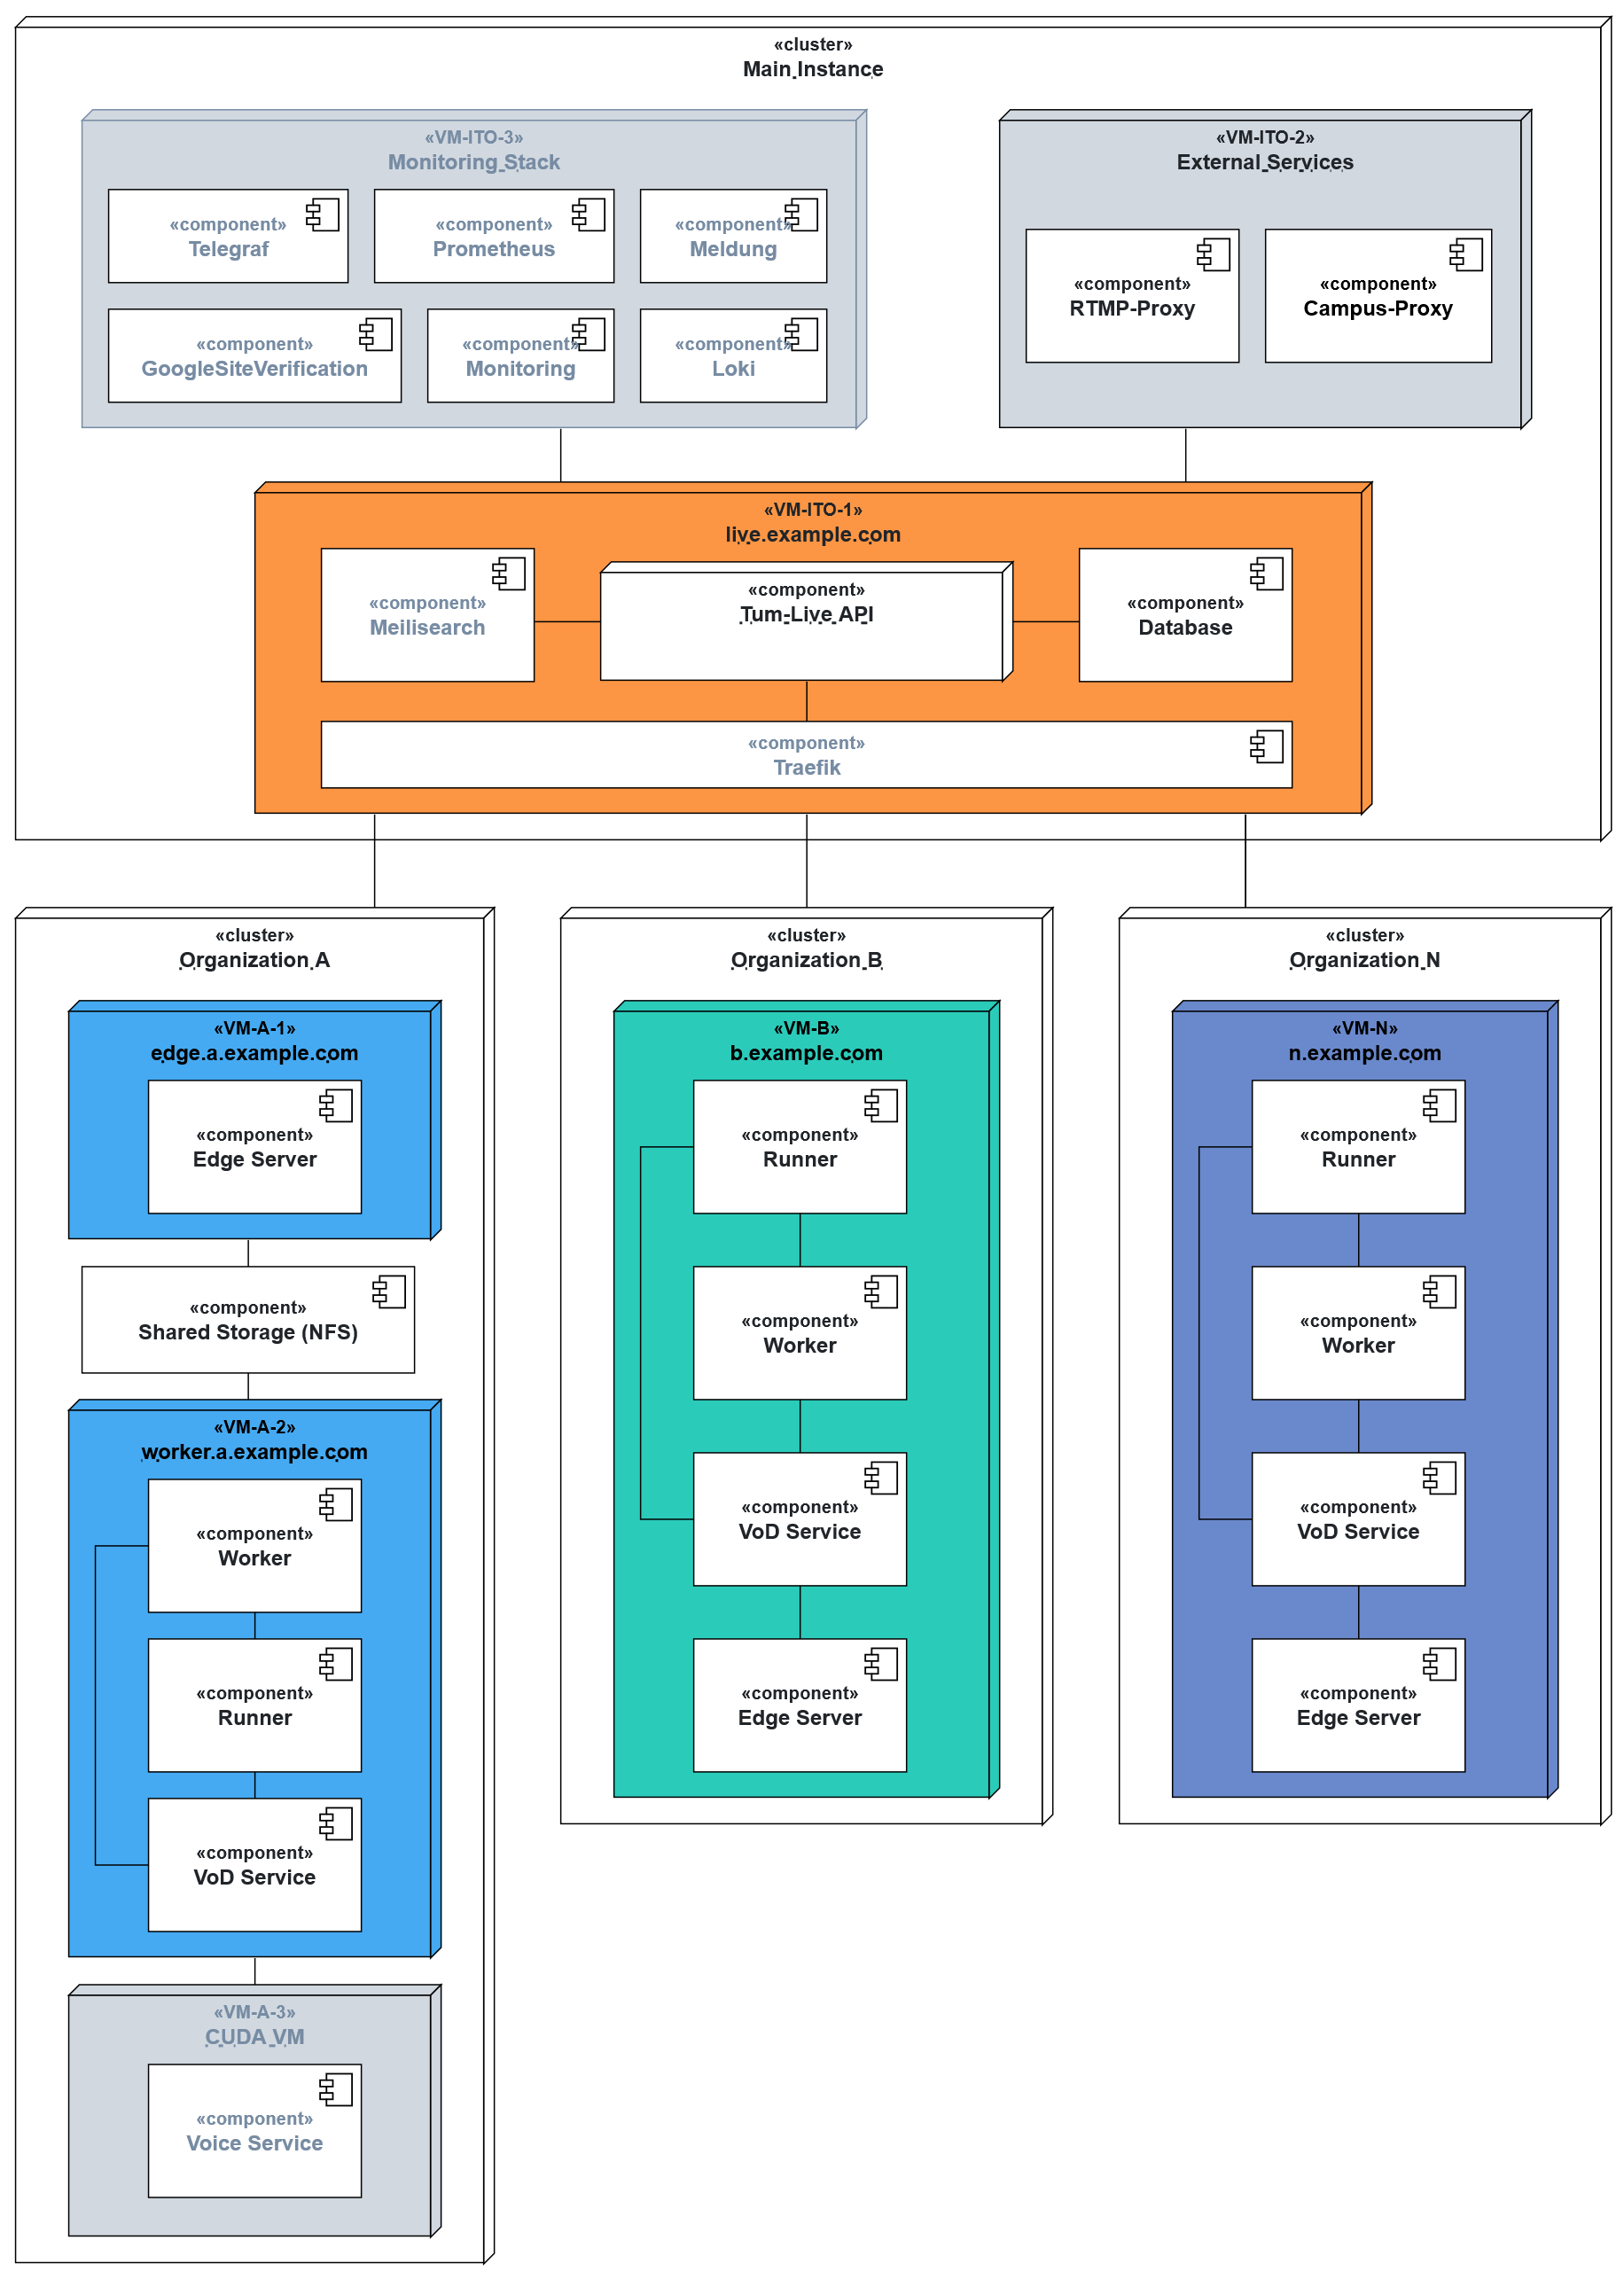
\includegraphics[width=400pt]{images/DeploymentDiagramNew.png}
    \caption[Target Deployment Diagram of TUM-Live]{Target Deployment Diagram of TUM-Live\footnotemark[5]}
    \label{fig:system-architecture}
\end{figure}

To distribute TUM-Live to different schools and universities, the subsystems and components responsible for processing and storing video data need to be distributed and hosted by each individual organization. 
The main TUM-Live \ac{API} instance however, will remain managed by the \ac{CIT} \ac{ITO} or \ac{TUM} so that users have a single point of access instead of having to switch instances when wanting to watch lectures of different schools.
To achieve this, each organization needs to host at least three components: the Worker component, the VOD Service component and an Edge Server. 
Each organization can decide how many resources it wants to allocate to each service depending on the expected load. The following minimum requirements are set:

\begin{itemize}
    \item At least 1 \ac{VM} as an Edge Server. This server serves the videos to the users. Throughput is important, so, to serve many users, more instances are needed.
    \item At least 1 Worker \ac{VM} to receive the stream and transcode the \ac{VOD}. On the same node, for every Worker a VOD Service needs to be deployed to expose a simple HTTP interface that accepts file uploads and packages them to a \ac{HLS} stream in a configured location. This stream may then be distributed by the Edge Server.
    \item Optionally, an organization can add additional \ac{VM}s for monitoring (\href{https://github.com/grafana/grafana}{Grafana}\footnote{\url{https://github.com/grafana/grafana}}, \href{https://github.com/prometheus/prometheus}{Prometheus}\footnote{\url{https://github.com/prometheus/prometheus}}, etc.) or for deploying services such as the Voice Service for subtitling live streams and \ac{VOD}s using the \href{https://github.com/openai/whisper}{Whisper LLM}\footnote{\url{https://github.com/openai/whisper}}.
\end{itemize}

\footnotetext[5]{In comparison to a \textit{System Architecture Model} (e.g., \autoref{fig:twitch-architecture} or \autoref{fig:system-architecture}), a \textit{Deployment Diagram} shows a concrete instance of an abstract system architecture.}

\section{Delegated Administration of Resources}\label{section:rbac}

Given the proposed system (see \autoref{fig:system-architecture}), this section documents how this system has been implemented and what the current limitations and potential improvements of the main user system are. 

\subsection{Updating Architecture and Core API}

As explained before, with increasing demand, GoCast needs to be extended for university-wide lecture streaming. The solution to this are \textbf{organizations} that allow for delegated partial administration of resources.

The first step of implementing this structure was updating GoCast's role system. Previously, it contained four roles: \texttt{admin}, \texttt{lecturer}, \texttt{student}, \texttt{visitor}. While admins can manage the entire system (e.g., create and delete lectures and users, as well as perform maintenance tasks), lecturers can only manage own or create new lectures and students only manage their own profile and preferences. However, with the introduction of organizations, this is not sufficient, as each organization needs to have own organization-scoped admins that can manage their organizations' resources without being able to interfere with other organizations. To do this, a new \texttt{maintainer} role has been introduced (see \autoref{fig:school-hierarchy}).
With this, an organization using GoCast is managed by a set of maintainers of this organization. A user with the \texttt{maintainer}-role can be maintainer of multiple organizations, and has also maintainer rights for all sub-organizations of his organizations.  
Maintainers also have some basic administrative functionality which is limited to their organizations' scope (e.g., create, update and delete courses and streams only for those organizations which are administered by that maintainer). 

\subsection{GoCast Organizations}

TUMOnline has a strict hierarchical structure for its organizations (one school has multiple departments; one department has multiple chairs; one chair has multiple courses ...).
%
% On a side node, TUMOnline has 7 organizations, 29 departments and 487 chairs.
While TUM-Live is mainly used by the TUM, in principle it does not need to differentiate between organizational types that strictly. Organizations are only relevant when it comes to distributing the live streams and recordings of a certain entity to that entity's resources (e.g., Workers and VOD Services). Hence, the introduction of GoCast's organizations which represent an entity responsible for processing data. In practice, this is most of the time a TUMOnline school, however, one can also create a GoCast organization for a department, chair or smaller organization which is subordinated to another organization, depending on the specific situation.

Here's an example to illustrate this in a more detailed way:
The TUMOnline "School of Management" (SOM) wants to start using TUM-Live. Hence, the SOM's IT team contacts the admins of TUM-Live who then create a new \textit{SOM organization} in TUM-Live and assign the SOM IT team as maintainers.
The subordinated "Chair of Financial Management and Capital Markets" (FA), however, has its own data center and wants to host its lectures with its own resources. In this case, either one of the SOM maintainers or the \ac{CIT} \ac{ITO} can create a new organization in TUM-Live as a sub-organization of the \textit{SOM organization} and accordingly assign new maintainers from the FA-team. Now, the the FA-maintainers have full control over their sub-organization and can connect their own resources from their data center with TUM-Live, independently of the SOM.

% The idea is the following: To avoid one entity having to manage and process all streaming data for the entire university (or multiple universities), GoCast is distributed to multiple entities. Each entity (aka GoCast 'organization') has so-called maintainers (users with the maintainer user role) that are allowed to manage the organization's resources such as Workers, VOD Services, etc.


% One maintainer can maintain multiple organizations.
% The following organization-related actions are allowed by a maintainer of an organization:

%     Create, update or delete organization

%     Create new tokens for that organization (required to add new resources)

%     Manage organization's resources

%     Manage organization's maintainers




\section{Distributed Resources}

Now that the user role system had been updated, the next step was to find a solution to have the different resources such as Workers connected to the main cluster of Workers independent of the others organizations' resources. However, at the same time, they should be able to process and distribute requests between each other regardless of the organization they are in. This section explains in detail how each subsystem works as part of the distributed GoCast system. 

\subsection{Workers and Runners}
To set up a distributed network of Workers, the first step was to update the system in such a way that Workers can be connected by an organization's maintainer to the main network of GoCast. To do this, an organization's maintainer can create a new organization-token, a \ac{JWT} that expires after seven hours and allows its owner to connect new resources for the organization. % (see \autoref{fig:school-token}).

% \begin{figure}[htpb]
%     \centering
%     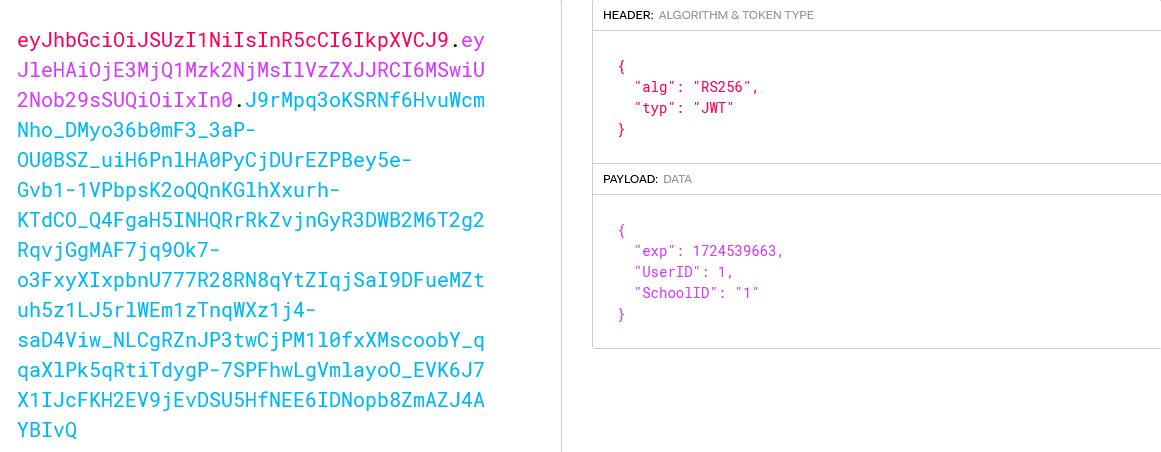
\includegraphics[width=390pt]{images/SchoolToken.png}
%     \caption[Example Organization Token]{Example Organization Token}\label{fig:school-token}
% \end{figure}

When a maintainer starts a new Worker, he can include this token in the containers environment (e.g., via a \texttt{docker-compose.yml} file or by passing it as an argument directly to Docker using \texttt{-e Token=<...>}). When starting up, the Worker sends a request to join the Worker pool of GoCast using the organization-token and additional data (e.g., host name, IP or FQDN address, \ac{VM} workload, etc.) and - if successful - receives a token without expiration which is then used to validate all subsequent requests from and to the Worker. Maintainers can then see and manage the current status of their registered resources in the Resource-Dashboard of GoCast (see \autoref{fig:resource-dashboard}).

\begin{figure}[htpb]
    \centering
    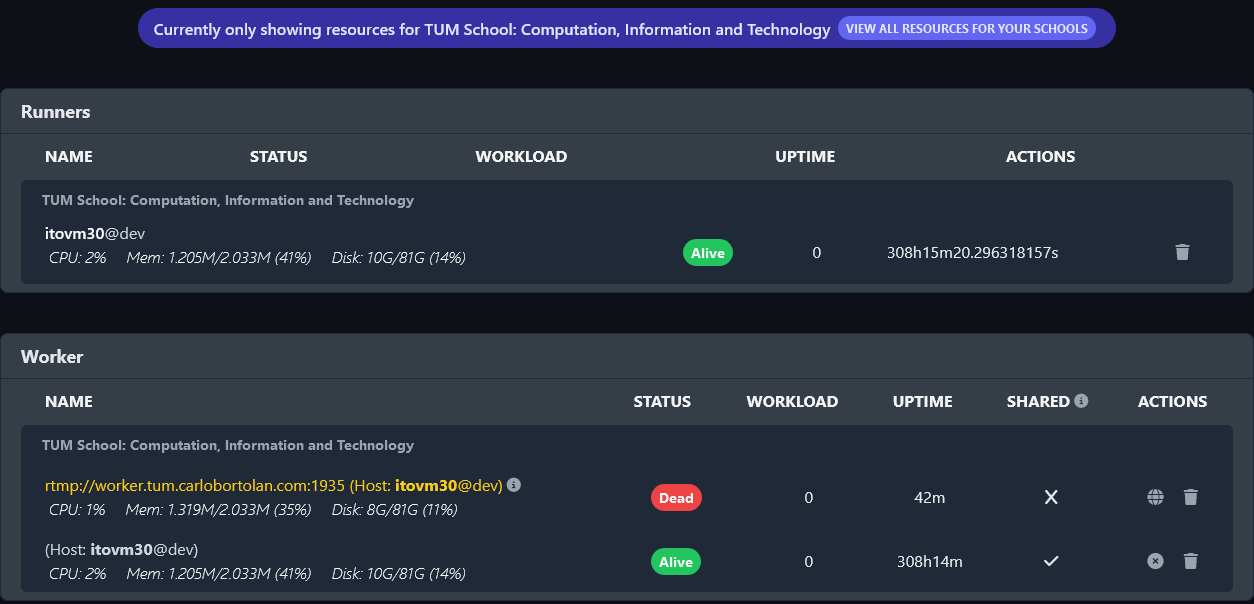
\includegraphics[width=390pt]{images/ResourceDashboard.png}
    \caption[Resources Dashboard]{Resources Dashboard}\label{fig:resource-dashboard}
\end{figure}

Now, whenever a new lecture is being received or uploaded, the main GoCast \ac{API} selects an available Worker for this organization and addresses it given the host name and IP address that the Worker has registered when first connecting to GoCast. For more details on how the distribution of tasks works, see \autoref{section:shared-resources}.

When the Worker receives such a request, it initiates the video transcoding process using \href{https://ffmpeg.org/}{FFmpeg}. The transcoding is performed based on the specific stream version\footnotemark[6]. 
The process is monitored in real-time, with progress being reported back to the GoCast system, to ensure that any failed actions are retried with backoff strategies and that the final transcoded video meets the expected duration and quality standards.

\footnotetext[6]{\texttt{CAM} streams use a higher compression level (CRF 26) and lower priority (niceness 10), while \texttt{PRES} streams use lower compression (CRF 20) and higher priority (niceness 9), with specific tuning in FFmpeg for still images in presentations. \texttt{COMB} streams, are assigned moderate compression (CRF 24) and the highest priority (niceness 8).}

\subsection{VOD Service and Edge Server}

Once the Worker has completed the transcoding process, the VOD Service starts detecting silent sections in the recordings so that the user will be able to skip these and jump directly to the start of the actual lecture. Then, it packages them into a \ac{HLS} stream and copies the packaged stream to the organization's recording storage.

To ensure easy access to these recordings, each organization also needs to have its own Edge Server set up. The VOD Service at each organization is responsible for managing the processing, packaging, and storage of the recordings server-side, while the Edge Server is responsible for distributing the streams to the end-users. This also has the advantage that each organization maintains full control over the storage of its streaming data.
Additionally, the Edge Server acts as a local cache for an organization's content. When students access recordings, the Edge Server distributes the content directly from the organization's storage, reducing the load on the organization's servers.

To allow for rapid post-processing and upload of \ac{VOD}s after a stream has ended, it is necessary that an organization has enough Workers to support the number of recorded lectures.
If an organization expects many concurrent viewers, it might need to consider having multiple Edge Servers running, as they have a limited bandwidth.
When network traffic to an Edge nodes exceeds the available bandwidth, the architecture might look like the example shown in \autoref{fig:edge-network}.

\begin{figure}[htpb]
    \centering
    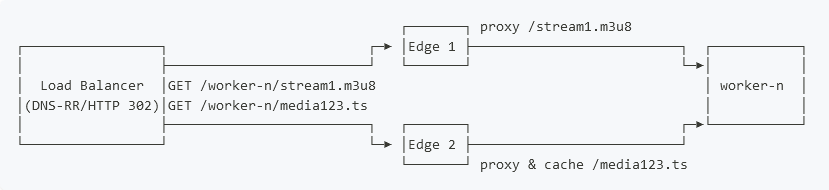
\includegraphics[width=\linewidth]{images/EdgeNetwork.png}
    \caption[Edge Server as proxy and cache node]{Edge Server as proxy and cache node}\label{fig:edge-network}
\end{figure}

% \subsection{Ingest Servers}
% TODO: How they are registered and distributed by the RTMP-Proxy
% \subsection{Voice Service}

\subsection{RTMP-Proxy}

\subsubsection{Limitaitons of GoCast's Selfstreaming}

GoCast supports not just recordings from the lecture hall or manual uploads, but also so-called self-streams. The idea behind self-streams is, that any lecturer can go live at any given time and stream from his own device without having to be in the lecture hall. In past, to do this, a lecturer had to go open TUM-Live, go to one his courses' page, select a lecture, and copy a link (such as: \texttt{rtmp://worker.example.com/cs-123? secret=5caa9d6447564cb5822995888e224f9a}) together with a secret stream key into a streaming software like OBS Studio. With the introduction of the organization system there are several reasons why this cannot work:

\begin{enumerate}
    \item The URL might change depending on the availability of Workers.
    \item Having to copy and paste a new URL every time a lecturer wants to start a stream can become annoying.
    \item For lecturers who teach at multiple organizations (e.g., a mathematics professor teaching lectures at the \ac{CIT} and at the School of Engineering and Design), managing different URLs for each organization would be inconvenient.
\end{enumerate}

\subsubsection{Proposed Solution and Data-Flow}

The solution for this is the RTMP-Proxy microservice. In a nutshell, the RTMP-Proxy acts as a router-like service that accepts all \ac{RTMP} self-stream requests and redirects them to an organization's Worker depending on the stream's course. With this, all a lecturer has to do is creating a new personal token (see \autoref{fig:personal-token}) and copy the token together with the target URL of the RTMP-Proxy into a streaming software only once.
After this initial setup, the lecturer can go live whenever they want by simply using the pre-configured URL and token.

\begin{figure}[htpb]
    \centering
    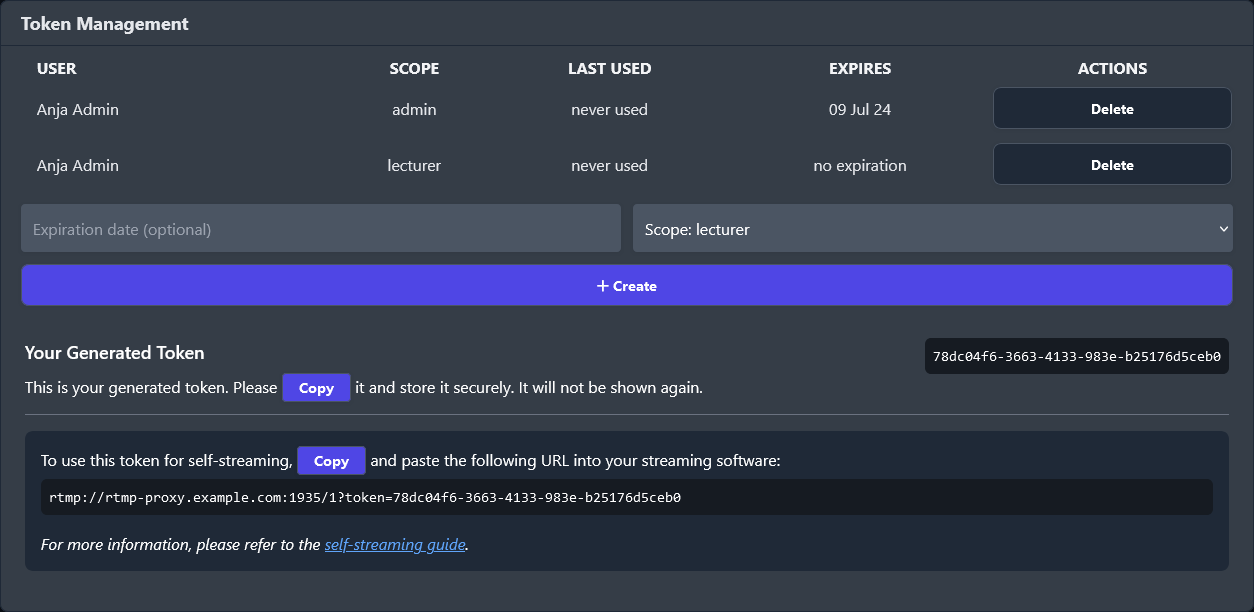
\includegraphics[width=\textwidth]{images/PersonalToken.png}
    \caption[Creation of Personal Token in TUM-Live and RTMP-Proxy URL]{Creation of Personal Token in TUM-Live and RTMP-Proxy URL}\label{fig:personal-token}
\end{figure}


The internal process of the RTMP-Proxy is as follows (see also \autoref{fig:rtmp-proxy}): 

\begin{enumerate}
    \item An incoming \ac{RTMP} request is received:\\
    \texttt{rtmp://proxy.example.com/live/<personal-token>}.
    \item The RTMP-Proxy sends a self-stream request to the main GoCast \ac{API} with the provided \texttt{personal-token}.
    \item The GoCast \ac{API} validates the \texttt{personal-token} and uses it to detect whether the lecturer has a scheduled lecture for the current time slot or a soon upcoming lecture and automatically starts the live stream with a waiting screen for viewers. Then it checks the stream's course's organization and returns the \ac{RTMP} URL of the ingest Worker currently available for that organization together with the course-slug and secret stream key for this stream: \\ 
    \texttt{rtmp://worker.example.com/<course-slug>?secret=<secret>/<secretKey>}.
    \item The RTMP-Proxy redirects the \ac{RTMP} request to the retrieved \ac{RTMP} URL.
    \item The organization's ingest Worker now receives the proxied \ac{RTMP} request as if it were sent directly to it by the lecturers streaming software.
\end{enumerate}

\begin{figure}[htpb]
    \centering
    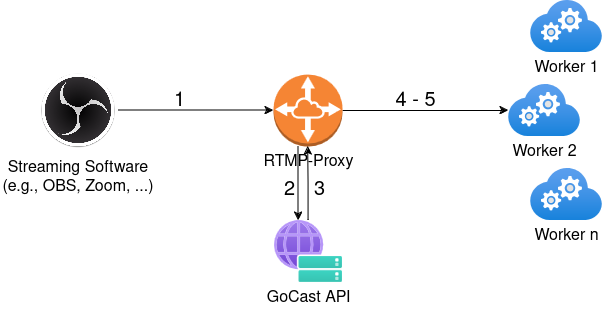
\includegraphics[width=300pt]{images/RtmpProxy.png}
    \caption[RTMP-Proxy Flow]{RTMP-Proxy Data Flow}\label{fig:rtmp-proxy}
\end{figure}

\subsubsection{Architectural Challanges and Limitations with RTMP}

Initially, for the prototype of the RTMP-Proxy the idea was to develop a microservice similar to the Edge Server or VOD Service written in Go that would redirect the \ac{RTMP} request (similar to a HTTP 302 redirect). However, after some testing, it quickly became obvious that Go does not have yet libraries to handle \ac{RTMP} requests with the necessary granularity. Hence, to proceed with this approach, it would require to use Go's native libraries to: 
\begin{itemize}
\item Handle the incoming \ac{RTMP} request
\item Perform a \ac{RTMP} handshake
\item Extract the user token from the \ac{RTMP} request
\item Find out the destination address
\item Establish a connection with the destination host
\item Streaming the video chunks directly to the destination address
\end{itemize}

\noindent This might work short term, but in the long term it would lead to other problems with potential bugs, scalability issues, complex error handling and unknown security vulnerabilities if not properly maintained.

A better solution was to use the \href{https://github.com/arut/nginx-rtmp-module}{nginx-rtmp-module}\footnotemark[7]\footnotetext[7]{\url{https://github.com/arut/nginx-rtmp-module}} that extends Nginx to handle \ac{RTMP} streaming requests natively~\parencite{nginx_rtmp_module}. 
Now, whenever a stream request arrives at the proxy server, Nginx accepts the request and invokes a script that extracts the stream key (the personal token) and requests the actual destination URL from the GoCast \ac{API}. Upon receiving the destination URL, Nginx pushes the stream to the target server.

\subsubsection{Implementation Details: FFmpeg vs OBS Compatibility}

During the testing phase, it was observed that at times streaming via FFmpeg worked perfectly fine, while attempts using OBS failed:
\begin{itemize}
    \item \textbf{Encoding Mismatch}: FFmpeg explicitly specifies H.264 for video and AAC for audio. OBS, however, may set different default codecs. The target \ac{RTMP} server of the Worker required H.264 video, and anything else would cause a rejection.
    \item \textbf{Keyframe Interval}: Workers generally expect a keyframe interval of around 2 seconds. OBS settings needed to be adjusted to enforce this interval.
    \item \textbf{Bitrate Mismatch}: High bitrate settings in OBS were causing overloads, which led to connection issues with the target \ac{RTMP} server. Lowering the bitrate resolved the issue.
    \item \textbf{URL Composition}: The self-streaming URL used to call the proxy is structured like: \texttt{<protocol>://<host>:<port>/live/<stream\_key>}. OBS however, requires the URL and stream key to be set separately (see \autoref{fig:obs-rtmp}).
\end{itemize}

\begin{figure}[htpb]
    \centering
    
\includegraphics[width=\linewidth]{images/OBSRTMP.png}
    \caption[OBS Settings for self-streaming]{OBS Settings for self-streaming}\label{fig:obs-rtmp}
\end{figure}

This was later fixed by changing the settings in OBS and setting the video encoder to \texttt{x264} (H.264), the audio encoder to \texttt{AAC}, adjusting the bitrate to a more reasonable level and settings the keyframe interval to 2 seconds for better compatibility with the Nginx \ac{RTMP} server.

\subsubsection{Final Words on Scaling the RTMP-Proxy}

While the RTMP-Proxy is far from perfect, it is meant as a prototype of a possible solution to stream via \ac{RTMP} using OBS in a distributed network where the final target address of the stream request is unknown when making the request. As the RTMP-Proxy is independent of other services in the GoCast environment (besides the main \ac{API} to receive the destination URL), it can be scaled very easily by deploying multiple RTMP-Proxies and having for example a Round-robin DNS distribute the load accordingly.

\section{Shared Resources}\label{section:shared-resources}

This section explains different approaches for the allocation of resources in the GoCast network. The main focus is on the task distribution to the available Workers when receiving new video upload or stream requests.

\subsection{Shared Resources}

Before explaining how resources in the GoCast Network are dynamically allocated to different tasks, it is first important to explain in detail how an organization actually "owns" a certain resource such as a Worker. As described in \autoref{section:rbac}, organizations are structured in a hierarchical manner. One organization can have multiple sub-organizations which can again have multiple sub-sub-organizations and so forth. When an organization has deployed its own resources, by default accessible only by the organization itself and its sub-organizations. Using the example shown in \autoref{fig:school-hierarchy}, this would mean that if there's a lecture uploaded by \textit{School 1}, only public resources and the organization's own private resources are considered. For a lecture of \textit{School 2a}, all public resources, the organization's own private resources as well as its parent-organization's resources (and recursively so on) are considered. 

\begin{figure}[htpb]
    \centering
    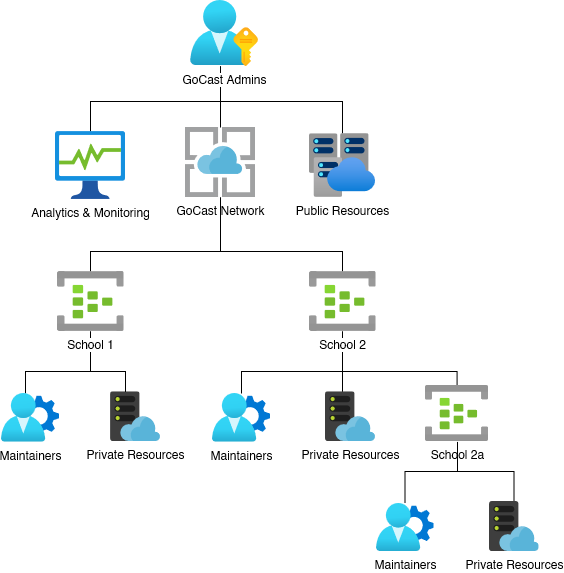
\includegraphics[width=250pt]{images/SchoolHierarchy.png}
    \caption[Example Organization Hierarchy]{Example Organization Hierarchy}\label{fig:school-hierarchy}
\end{figure}

Additionally, for certain resources, for example Workers, one can decide to set the \texttt{Shared} flag. When a resource has that flag enabled, it means that even though it is part of an organization (and hence by default only available for lectures of that organization or sub-organizations in that organization's hierarchy), it now becomes available to all organizations and shares its compute power with the entire network of organizations. To use the previous example, assuming that \textit{School 2a} has allowed to shared its resources, when \textit{School 1} uploads a video or starts a stream, in addition to its own private resources and the public resources, it also considers the shared resource of \textit{School 2a}.

\subsection{Four Approaches for Task Distribution}

The following are four approaches considered for the decision algorithm behind the allocation of resources - especially of Workers - in the GoCast Network. The current implementation for the task distribution of Workers uses the second approach. For the Runners, it remains to be seen which approach will be chosen - most likely a combination of the second and third approach. 

% \begin{enumerate}
    % \item \textbf{Randomized Allocation:}  
\subsubsection{1. Randomized Allocation}
     Tasks are assigned to available resources randomly. This method is simple and helps to distribute tasks across resources in an unbiased manner. However, it only considers a organization's own and public resources, ignoring the hierarchical structure of organizations or resource workloads. Randomized allocation can be effective if resource capabilities were relatively uniform, but it would most likely lead to inefficiencies if the networks got more complex.

    \begin{figure}[htpb]
      \begin{tabular}{c}
      \ \small \begin{lstlisting}[language=SQL]
        -- 1. Randomized allocation example query
        SELECT *
        FROM workers 
        WHERE shared = TRUE OR org_id = ?
        ORDER BY RANDOM()
        LIMIT 1;
        \end{lstlisting}
      \end{tabular}
      \label{fig:randomized-allocation}
    \end{figure}
    
    % \item \textbf{Recursive Organization-Based Allocation:}  
\subsubsection{2. Recursive Organization-Based Allocation}
    When a task is started, the system recursively checks for available resources, starting from the organization's own resources and moving up the hierarchy to include parent organizations and shared resources as described in the previous subsection. This guarantees that each task is allocated to the most appropriate resource, improving resource utilization across the network by allowing sub-organizations to benefit from the resources of their parent organizations, while respecting the resource ownership of each organization. One could implement different optimizations such as prioritizing own resources before shared resources or limit how many levels the query should follow the parent-child relationship upwards. Also, one organization might not want to use resources shared by other organizations and therefore include only resources from its own organization's hierarchy. The code snippet below is an example of how a recursive query might look like to find all available Workers in an organization's hierarchy including shared Workers.   

    \begin{figure}[htpb]
      \begin{tabular}{c}
      \ \small \begin{lstlisting}[language=SQL]
        -- 2. Recursive organization-based allocation example query
        -- First, create a recursive query to follow the parent-child hiarachy upward
        WITH RECURSIVE org_hierarchy AS (
            SELECT id, parent_id FROM orgs WHERE id = ?
            UNION ALL
            SELECT o.id, o.parent_id FROM orgs o
            INNER JOIN org_hierarchy oh ON o.id = oh.parent_id 
        ) 
        -- Then, select all Workers that are in the hiararchy or shared
        SELECT w.* FROM workers w
        LEFT JOIN org_hierarchy oh ON oh.id = w.org_id
        WHERE oh.id IS NOT NULL OR w.shared = true;
        \end{lstlisting}
      \end{tabular}
      \label{fig:recursive-allocation}
    \end{figure}

    % \item \textbf{Priority-Based Allocation:}  
\subsubsection{3. Priority-Based Allocation}
    Tasks are assigned to Workers based on a dynamically adjusted priority queue. The tasks would be prioritized based on factors such as viewer count, failure rate, \ac{VM} workload or the type of content being processed. For example, live streaming tasks could be given a higher priority over \ac{VOD} uploads and hence be processed by a Worker that runs on a more powerful \ac{VM}. This approach would assign critical tasks (e.g., live streaming) first, and re-schedule less urgent tasks (e.g., \ac{VOD} uploads or thumbnail generation) for later. The example below shows one possible implementation of the selection process assuming that the \texttt{taskQueue} contains tasks sorted by priority. 

    \begin{figure}[htpb]
      \begin{tabular}{c}
      \ \small \begin{lstlisting}[language=Java]
        // 3. Priority-based allocation pseudocode
        function processTaskQueue(taskQueue) {
            while not taskQueue.isEmpty() {
                task = taskQueue.dequeue() // Get task with highest priority
                worker := getNextAvailableWorker() // Find available Worker
                if worker != nil {
                    worker.assignTask(task)
                } else {
                    taskQueue.enqueue(task) // Requeue task if no Workers are available
                }
            }
        }
        \end{lstlisting}
      \end{tabular}
      \label{fig:priority-based-allocation}
    \end{figure}

\subsubsection{4. Linear Programming Optimization Approach}

By setting up and solving a \ac{LP}, the tasks can be distributed evenly among Workers in such a way that the maximum load on any single worker is minimized and bottlenecks are reduced.

\begin{enumerate}
    \item \textbf{Variables and Parameters}

Let:
\begin{itemize}
    \item \( n \) be the number of tasks.
    \item \( m \) be the number of Workers.
    \item \( t_i \) be the processing time of task \( i \) estimated using past averages or heuristics based for example on scheduled stream's duration.
    \item \( x_{ij} \) be a binary decision variable, where \( x_{ij} = 1 \) if task \( i \) is assigned to Worker \( j \), and \( x_{ij} = 0 \) otherwise.
    \item \( L_j \) be the total workload on Worker \( j \), calculated as \( L_j = \sum_{i=1}^{n} t_i \cdot x_{ij} \).
    % \item \( L_{\text{max}} \) be the maximum load across all Workers, defined as \( L_{\text{max}} = \max_{j=1}^{m} L_j \).
\end{itemize}

\item \textbf{Objective Function}

The objective is to minimize the maximum load \( L_{\mathrm{max}} \) across all Workers:
\begin{equation}
\operatorname{Minimize\ } L_{\text{max}}
\end{equation}

\item \textbf{Constraints}

The \ac{LP} is subject to the following constraints:

\begin{enumerate}
    \item \textbf{Task Assignment:} Each task \( i \) must be assigned to exactly one Worker:
    \begin{equation}
    \sum_{j=1}^{m} x_{ij} = 1 \quad \forall i = 1, \dots, n
    \end{equation}

    \item \textbf{Load Calculation:} The workload of each Worker \( j \) is the sum of the processing times of the tasks assigned to that Worker:
    \begin{equation}
    L_j = \sum_{i=1}^{n} t_i \cdot x_{ij} \quad \forall j = 1, \dots, m
    \end{equation}

    \item \textbf{Bounding the Maximum Load:} The workload on each Worker must be less than or equal to the maximum load \( L_{\text{max}} \):
    \begin{equation}
    L_j \leq L_{\text{max}} \quad \forall j = 1, \dots, m
    \end{equation}
    
    \item \textbf{Binary Variables:} The assignment variables \( x_{ij} \) are binary:
    \begin{equation}
    x_{ij} \in \{0, 1\} \quad \forall i = 1, \dots, n \quad \text{and} \quad \forall j = 1, \dots, m
    \end{equation}
\end{enumerate}

\item \textbf{Linear Programming Formulation:}

Given the objective function and the constraints, the solution to the \ac{LP} can be formulated as:
\begin{align}
\text{Minimize} \quad & L_{\text{max}} \\
\text{subject to} \quad & \sum_{j=1}^{m} x_{ij} = 1 \quad \forall i = 1, \dots, n \\
& L_j = \sum_{i=1}^{n} t_i \cdot x_{ij} \quad \forall j = 1, \dots, m \\
& L_j \leq L_{\text{max}} \quad \forall j = 1, \dots, m \\
& x_{ij} \in \{0, 1\} \quad \forall i = 1, \dots, n \quad \text{and} \quad \forall j = 1, \dots, m
\end{align}
\item \textbf{Example Implementation:} 

    \begin{figure}[htpb]
      \begin{tabular}{c}
      \ \small \begin{lstlisting}[language=Python]
        # Using Gurobi as an example - any other solver also works
        from gurobipy import Model, GRB, quicksum
        model = Model("Minimize_Max_Load")
        
        # Decision variables: x[i, j] = 1 if task i is assigned to Worker j, 0 otherwise
        x = model.addVars(n, m, vtype=GRB.BINARY, name="x")
        
        # Variable for maximum load across all Workers
        L_max = model.addVar(vtype=GRB.CONTINUOUS, name="L_max")
        
        # Objective: Minimize the maximum load L_max
        model.setObjective(L_max, GRB.MINIMIZE)
        
        # Constraint 3.a) Each task is assigned to exactly one Worker
        for i in range(n):
            model.addConstr(
                quicksum(x[i, j] for j in range(m)) == 1, name=f"Task_Assignment_{i}")
        
        # Constraint 3.b) and 3.c) Load on each Worker does not exceed L_max
        for j in range(m):
            model.addConstr(
                quicksum(t[i] * x[i, j] for i in range(n)) <= L_max, 
                name=f"Worker_Load_{j}")
        
        # Run the model
        model.optimize()
        \end{lstlisting}
      \end{tabular}
      \label{fig:lp-optimization}
    \end{figure}

\end{enumerate}

%% !TeX root = ../main.tex
% !TeX root = ../main.tex
% Add the above to each chapter to make compiling the PDF easier in some editors.

\chapter{Scaling Resources Vertically}\label{chapter:introduction}

\section{VM Upscaling and Other Approaches}
TODO
% !TeX root = ../main.tex
% !TeX root = ../main.tex
% Add the above to each chapter to make compiling the PDF easier in some editors.

\chapter{Performance Optimization and Error Analysis}\label{chapter:optimization_and_alternative_technologies}

This chapter presents an insight into collected log and error metrics, a detailed analysis of the performance of GoCast's Workers, as well as an optimization approach for the main GoCast\ac{API} that compares the current REST \ac{API} with a prototype of a gRPC \ac{API}.   

\section{Monitoring Stack}

The GoCast system uses a rather complex stack of monitoring, logging, and analytics tools to collect metrics. The main technologies include \href{https://github.com/grafana/grafana}{Grafana}, \href{https://github.com/prometheus/prometheus}{Prometheus}, \href{https://github.com/influxdata/telegraf}{Telegraf}, and \href{https://github.com/influxdata/influxdb}{InfluxDB}, which are deployed in a containerized environment using Docker and managed by \href{https://github.com/traefik/traefik}{Traefik} as a reverse proxy. The collected data is then organized into Grafana dashboards. The metrics collection and logging system for TUM-Live is based on the following main components:
\begin{itemize}
    \item \textbf{\href{https://github.com/grafana/grafana}{Grafana}}\footnote{\url{https://github.com/grafana/grafana}}: This is used as the main dashboard for visualizing metrics and performance of connected services in real-time.
    \item \textbf{\href{https://github.com/prometheus/prometheus}{Prometheus}}\footnote{\url{https://github.com/prometheus/prometheus}}: As a monitoring and alerting toolkit, Prometheus is responsible for scraping metrics from the various services within the system.
    \item \textbf{\href{https://github.com/influxdata/telegraf}{Telegraf}}\footnote{\url{https://github.com/influxdata/telegraf}}: Collects metrics and logs from Docker containers, the host system, and various applications. It works together with InfluxDB to store time-series data.
    \item \textbf{\href{https://github.com/influxdata/influxdb}{InfluxDB}}\footnote{\url{https://github.com/influxdata/influxdb}}: A time-series database, InfluxDB is utilized for storing logs and metrics collected from Telegraf, which are then visualized through Grafana.
    \item \textbf{\href{https://github.com/grafana/loki}{Loki}} and \textbf{\href{https://grafana.com/docs/loki/latest/send-data/promtail/}{Promtail}}\footnote{\url{https://github.com/grafana/loki}}: These tools are used for centralized logging, allowing for real-time querying and log analysis through Grafana's Loki integration.
    % \item \textbf{\href{https://mariadb.org/}{MariaDB}}: Used as the primary database for storing TUM-Live application data and internal user stats (see \autoref{subsection:user-stats-tumlive}).
\end{itemize}

\section{Metrics of the GoCast API}

The main data source for the GoCast \ac{API} are Loki and Traefik as well as internal server logs. This section will give some insights on common errors and patterns found in the main \ac{API} and (given the limited amount of logging data) focus on two main aspects: The number of errors and the observed errors types. The Python scripts for the plots for this and the following sections be found at \href{https://github.com/carlobortolan/thesis/tree/analytics}{github.com/carlobortolan/thesis/analytics}.

\subsection{Error Volume Analysis}

Plotting the logged errors of the \ac{API} over time (see \autoref{fig:api-cum-errors-over-time}) shows an increase in the sum of total \ac{API} errors with a constant, positive slope. This indicates that errors were being logged at a relatively similar rate throughout the observed period. The fact that there are no obvious sudden spikes or drops in this data suggests a continuous, recurring issue rather than isolated incidents. Since the slope did not flatten over time, it shows that the error volume did not escalate or improve significantly over time, implying that either no major fixes were implemented to resolve the underlying causes during this time frame or new bugs were introduced with prior fixes.

\begin{figure}[htpb]
    \centering
    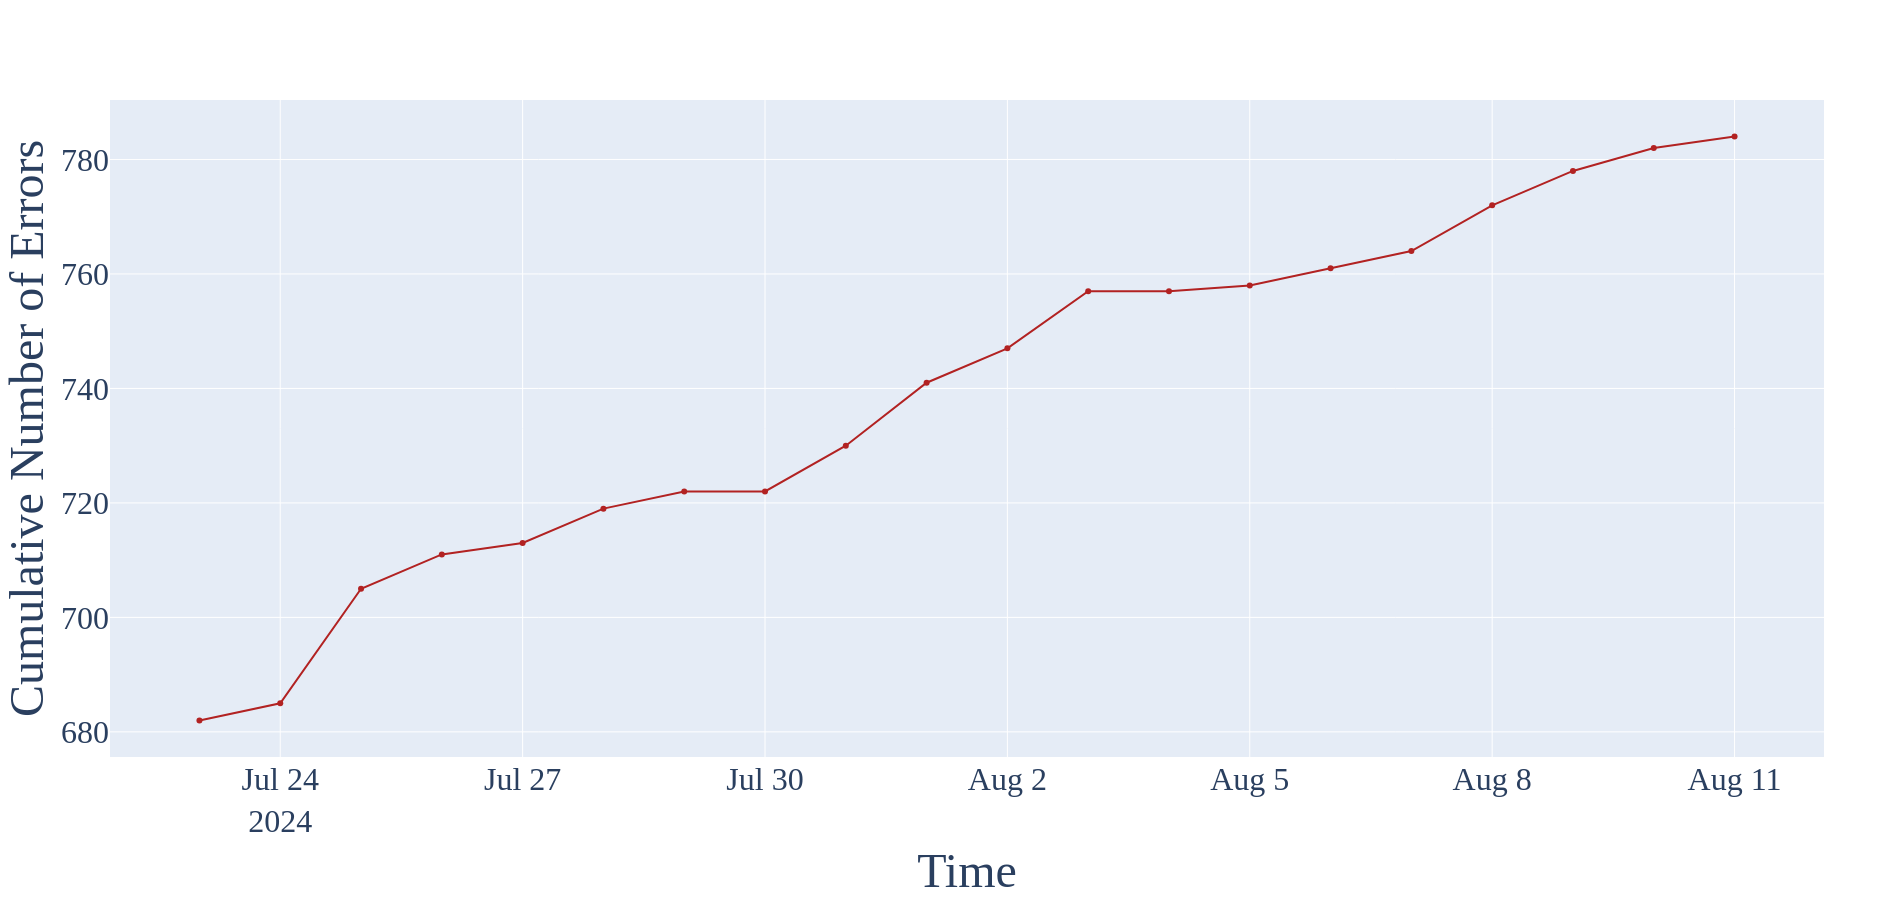
\includegraphics[width=\linewidth]{images/plots/api/cum_errors_over_time.png}
    \caption[Cumulative \ac{API} Errors Over Time]{Cumulative \ac{API} Errors Over Time}\label{fig:api-cum-errors-over-time}
\end{figure}

% \begin{figure}[htpb]
%     \centering
%     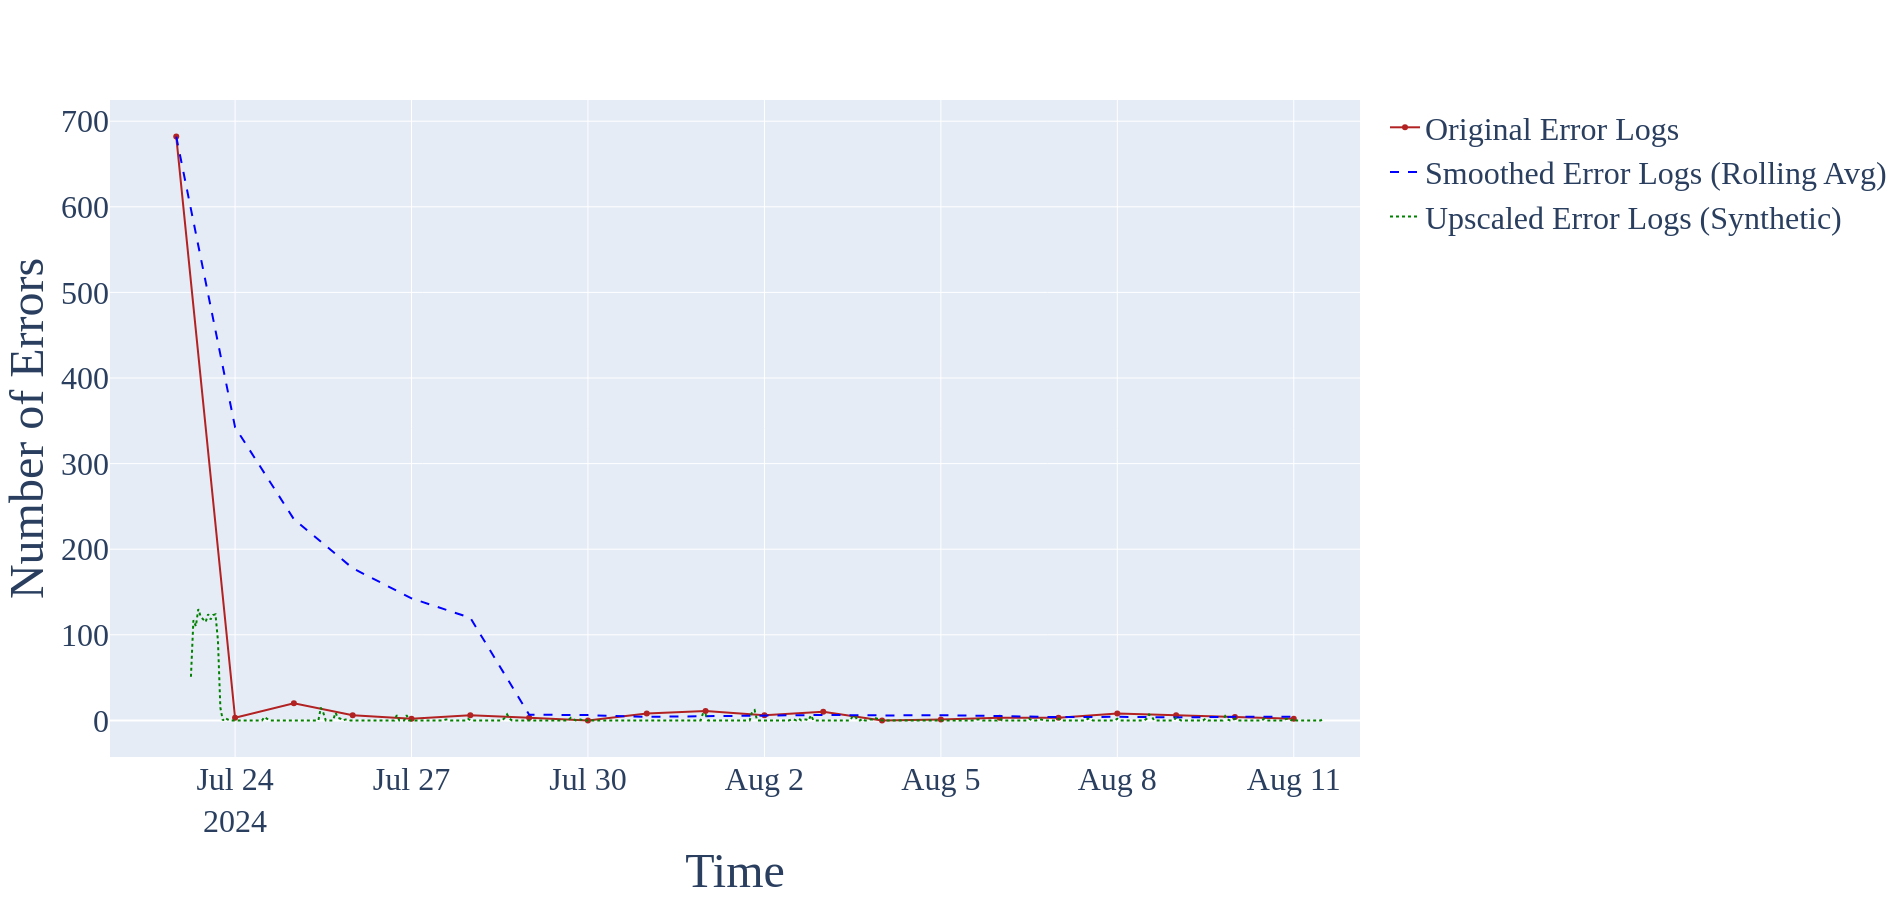
\includegraphics[width=\linewidth]{images/plots/api/upscaled_error_logs.png}
%     \caption[Upscaled \ac{API} Error Logs]{Upscaled \ac{API} Error Logs}\label{fig:api-upscaled-error-logs}
% \end{figure}

\subsection{Categorization of Error Types}

The errors are not logged with a specific error type, but they contain a JSON String from which one can infer the origin of the error (e.g., see \autoref{fig:api-error-json}).

\begin{figure}[htpb]
  \begin{tabular}{c}
  \ \small \begin{lstlisting}[language=Java]
    {
      "time": "2024-07-23T06:38:08.282288184+02:00",
      "level": "ERROR",
      "msg": "Could not generate live preview",
      "service": "api",
      "err": "rpc error: code = Unknown desc = exit status 1"
    }
    \end{lstlisting}
  \end{tabular}
  \caption[Example \ac{API} Error JSON]{Example \ac{API} Error JSON}\label{fig:api-error-json}
\end{figure}

\noindent As seen in \autoref{fig:api-error-types}, the most common error logged by the \ac{API} was \textit{'Could not generate live preview'} with 677 occurrences. To understand this error, first it is necessary to explain that GoCast allows admins to trigger certain cron jobs which then periodically perform a certain action such as importing course-assignments from CAMPUSonline, or in this case - fetching the thumbnails of live streams (Live Previews) from the GoCast Workers. Hence, this error is a result of the \texttt{FetchLivePreviews} cron job which is performed every minute to get a live thumbnail from a Worker. If this request returns an error, it logs the  ends the connection and decrements the Worker's workload. Possible reasons for this could be network issues preventing the communication with the Worker, general Worker unavailability, or invalid or incomplete parameters passed to the \texttt{getLivePreviewFromWorker} function.

\begin{figure}[htpb]
    \centering
    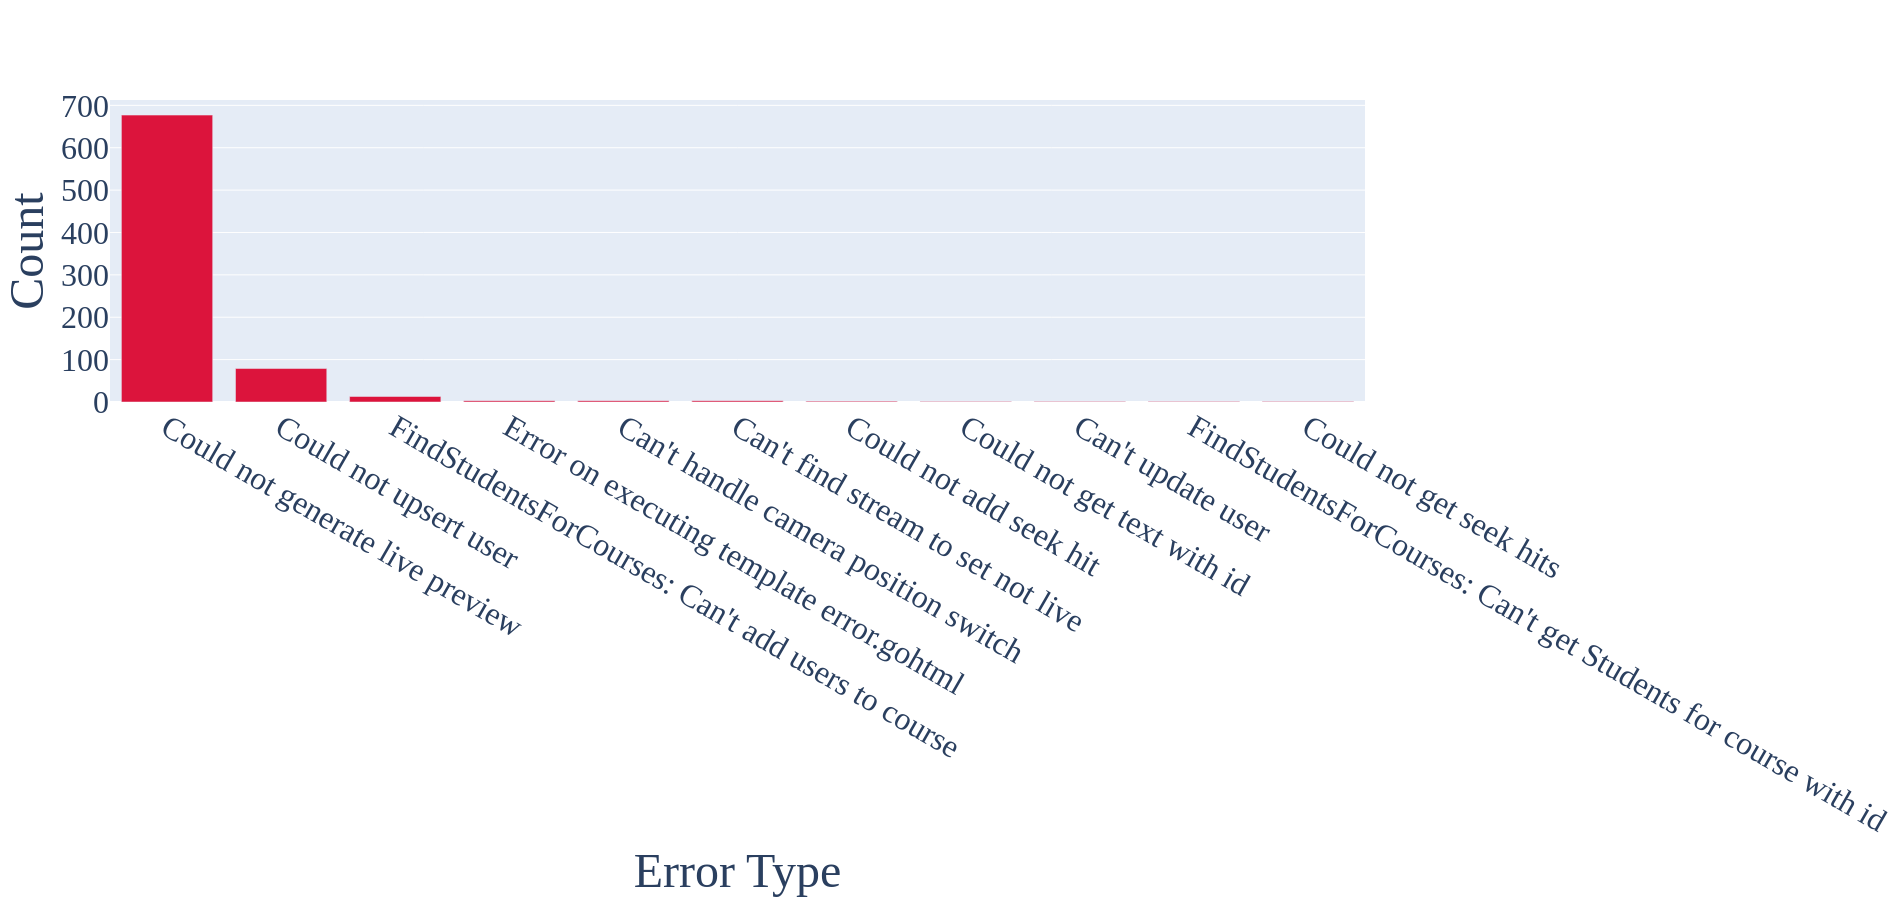
\includegraphics[width=\linewidth]{images/plots/api/error_types.png}
    \caption[\ac{API} Error Types]{\ac{API} Error Types}\label{fig:api-error-types}
\end{figure}
\break

\noindent When aggregating the errors by their hour and plotting them in a bar chart grouped by error type (\autoref{fig:api-errors-by-hour-and-type}), there's an interesting observation that the \textit{'Could not generate live preview'} error, which is the most common error, mainly occurs during normal lecture times from 6AM to 5PM. As the number of reported occurrences of this error is constant over these hours, it can be assumed that it is either an issue with an individual Worker that might have a connection issue or is running an outdated docker image (the log data does not provide information on which \ac{VM} the error occurred), or a bug that affects all Workers. However, since we know that the \ac{API} fetches the previews once every minute from all Workers, and the number of errors per hour is around 60, it is most likely an issue with one individual Worker. If the issue was a random connection error, the number of occurrences should vary significantly and if the issue was a system-wide misconfiguration or bug in the Worker microservice, the error should occur on all Workers, meaning that the number of errors should be: \texttt{number of Workers * 60}.     

\begin{figure}[htpb]
    \centering
    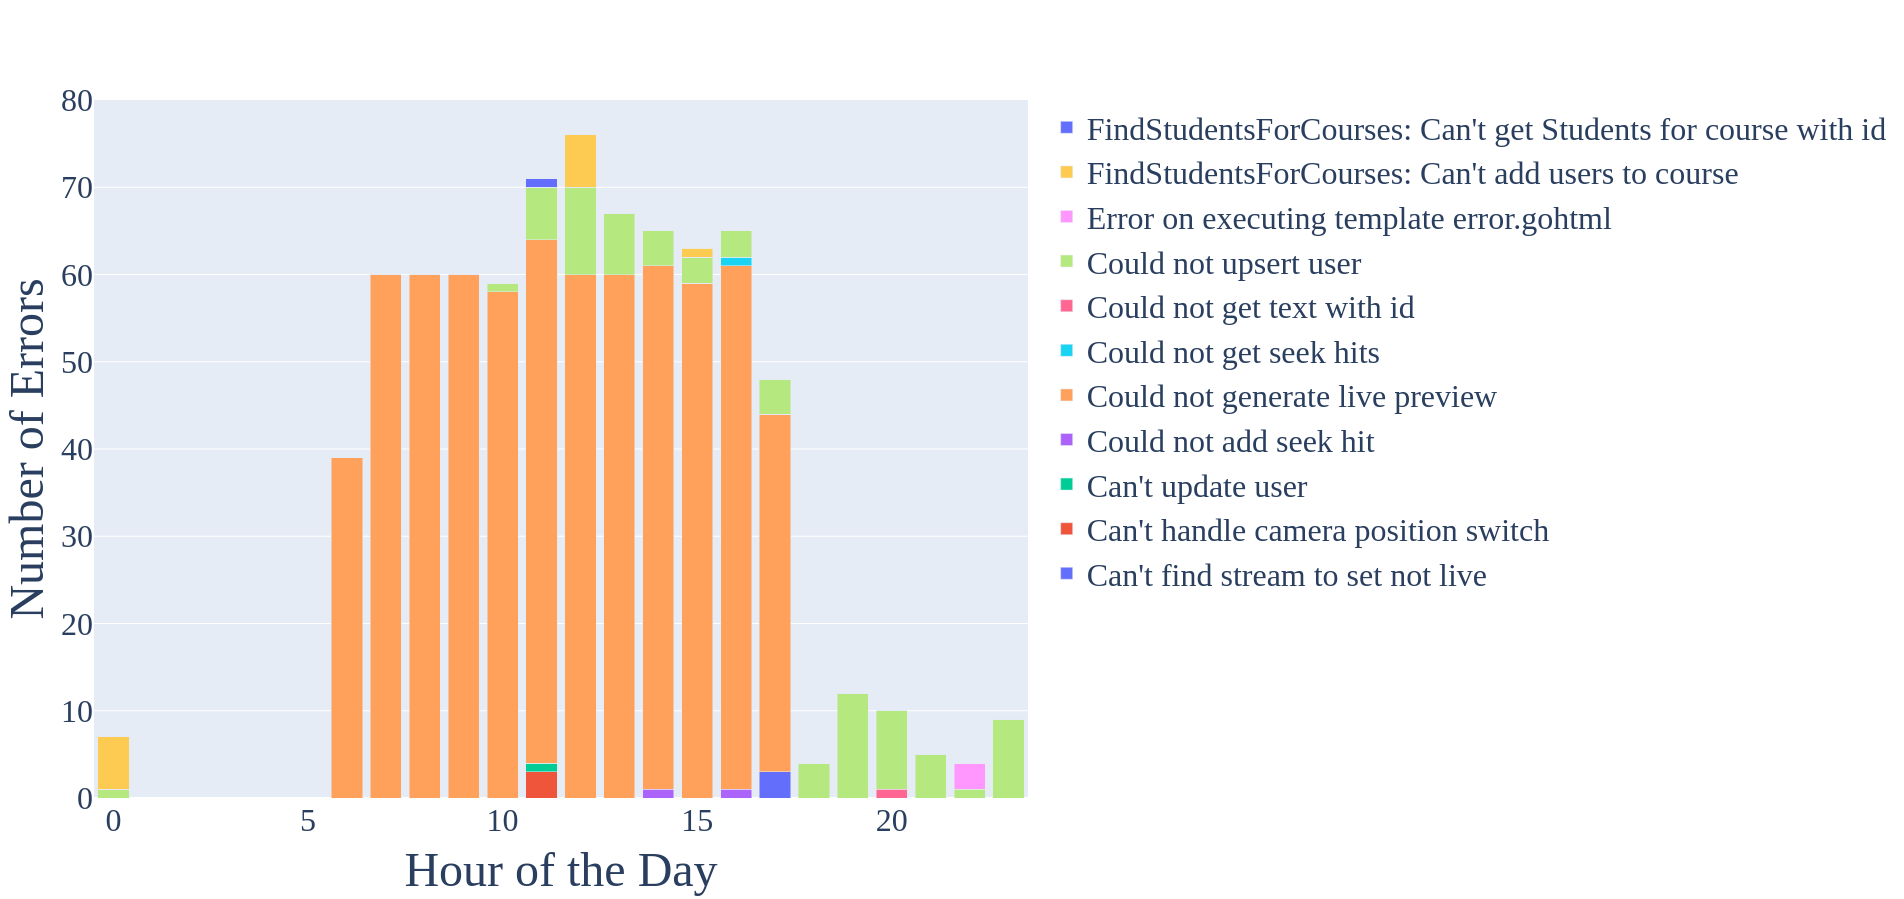
\includegraphics[width=\linewidth]{images/plots/api/errors_by_hour_and_type.png}
    \caption[\ac{API} Errors by Hour and Type]{\ac{API} Errors by Hour and Type}\label{fig:api-errors-by-hour-and-type}
\end{figure}

% \begin{figure}[htpb]
%     \centering
%     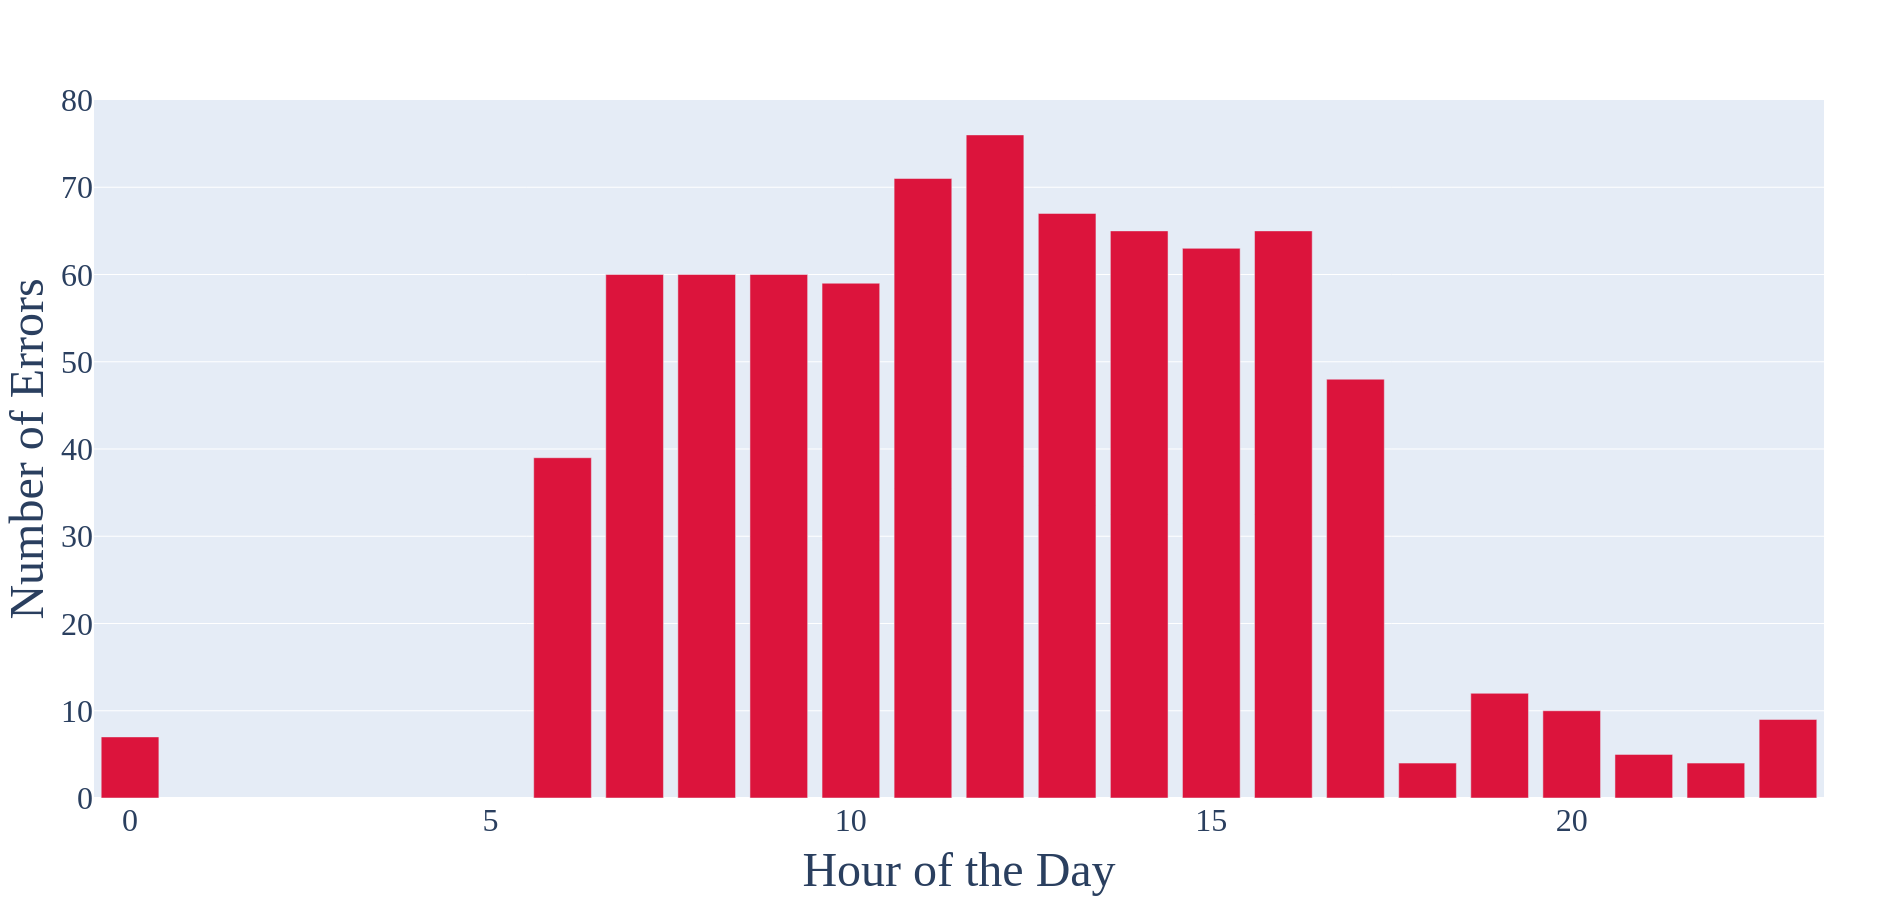
\includegraphics[width=\linewidth]{images/plots/api/errors_by_hour.png}
%     \caption[\ac{API} Errors by Hour]{\ac{API} Errors by Hour}\label{fig:api-errors-by-hour}
% \end{figure}

\section{Performance Bottleneck: Worker}

Again, using data collected from various logging services and exported via GoCast's Grafana dashboard, this section will give some insights on common errors of the Worker microservice and try to find possible causes as well as potential solutions to either avoid these errors or make it easier to debug them in the future.  

\subsection{Errors over Time}

Similarly to the main \ac{API}, the Worker logs too show a constant number of errors over time (see \autoref{fig:worker-cum-errors-over-time}) indicating that there are either bugs or network issues that continue to occur without being solved. With an average of approximately 30 Worker-related errors per day and days with as much as 75 logged errors (see \autoref{fig:worker-upscaled-error-logs} it shows that the Worker system can become a bottleneck in the future. Especially considering that - in contrast to the main \ac{API} - there is not just one Worker deployed, but rather a few dozens, meaning that the number of errors will increase proportionally to the number of Workers deployed. 

\begin{figure}[htpb]
    \centering
    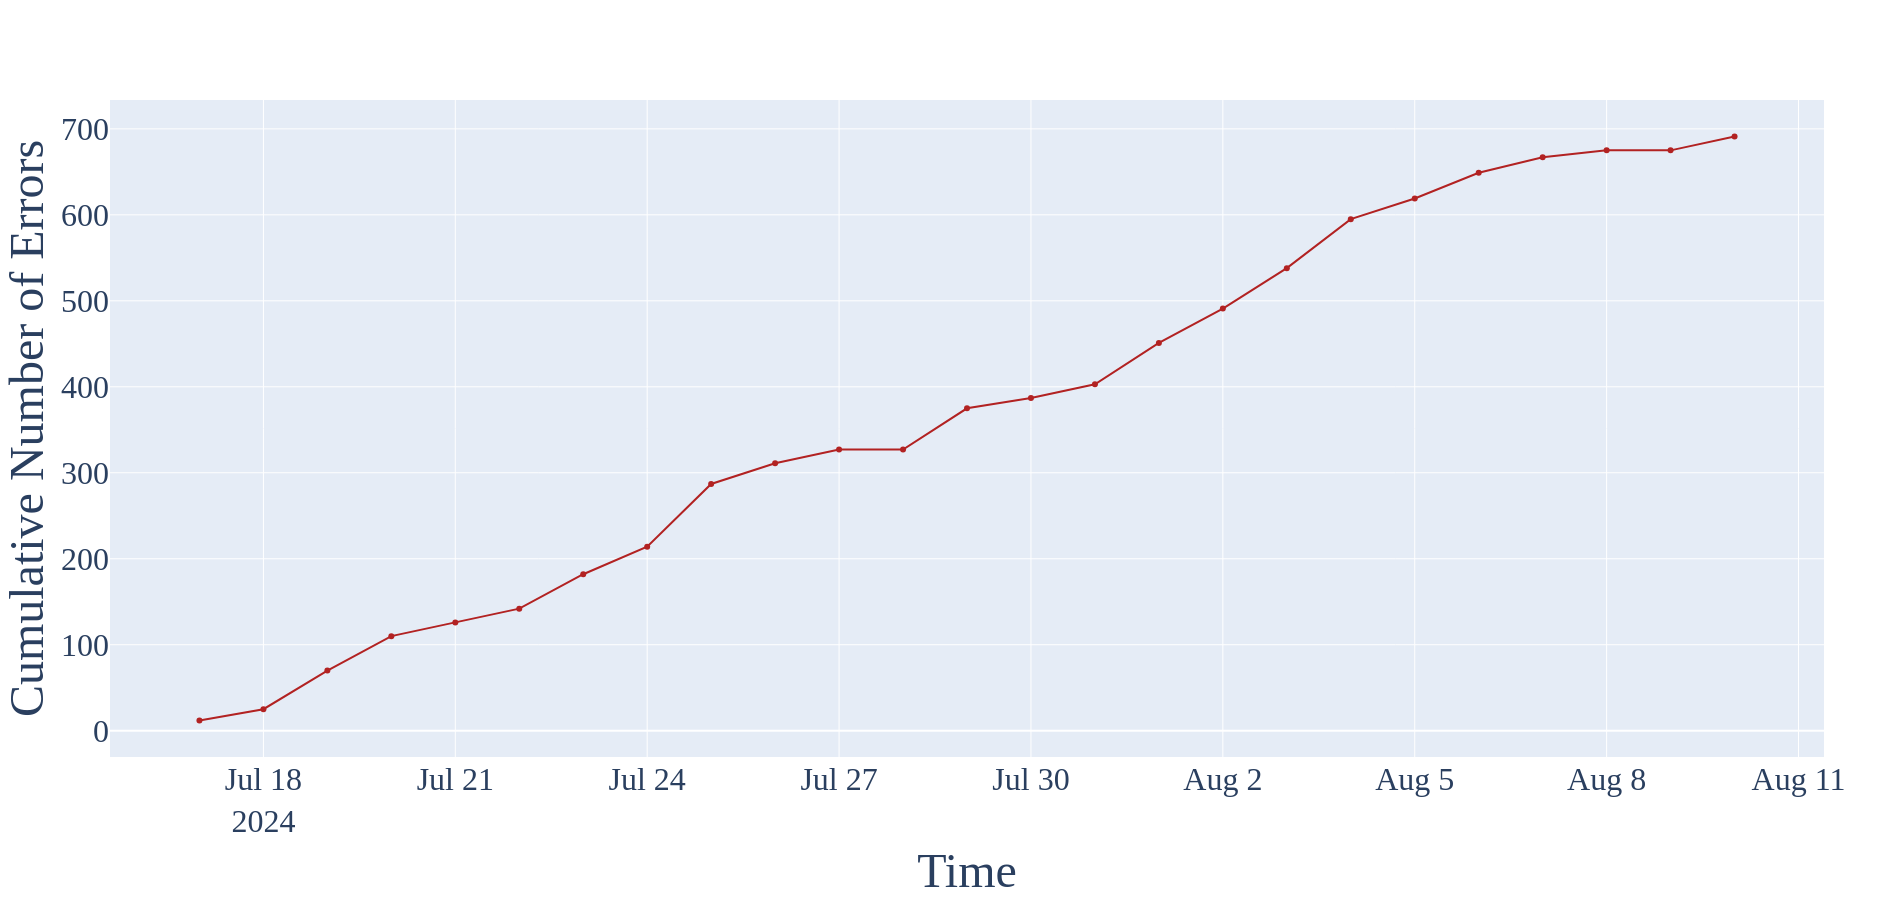
\includegraphics[width=\linewidth]{images/plots/worker/cum_errors_over_time.png}
    \caption[Cumulative Worker Errors Over Time]{Cumulative Worker Errors Over Time}\label{fig:worker-cum-errors-over-time}
\end{figure}

\begin{figure}[htpb]
    \centering
    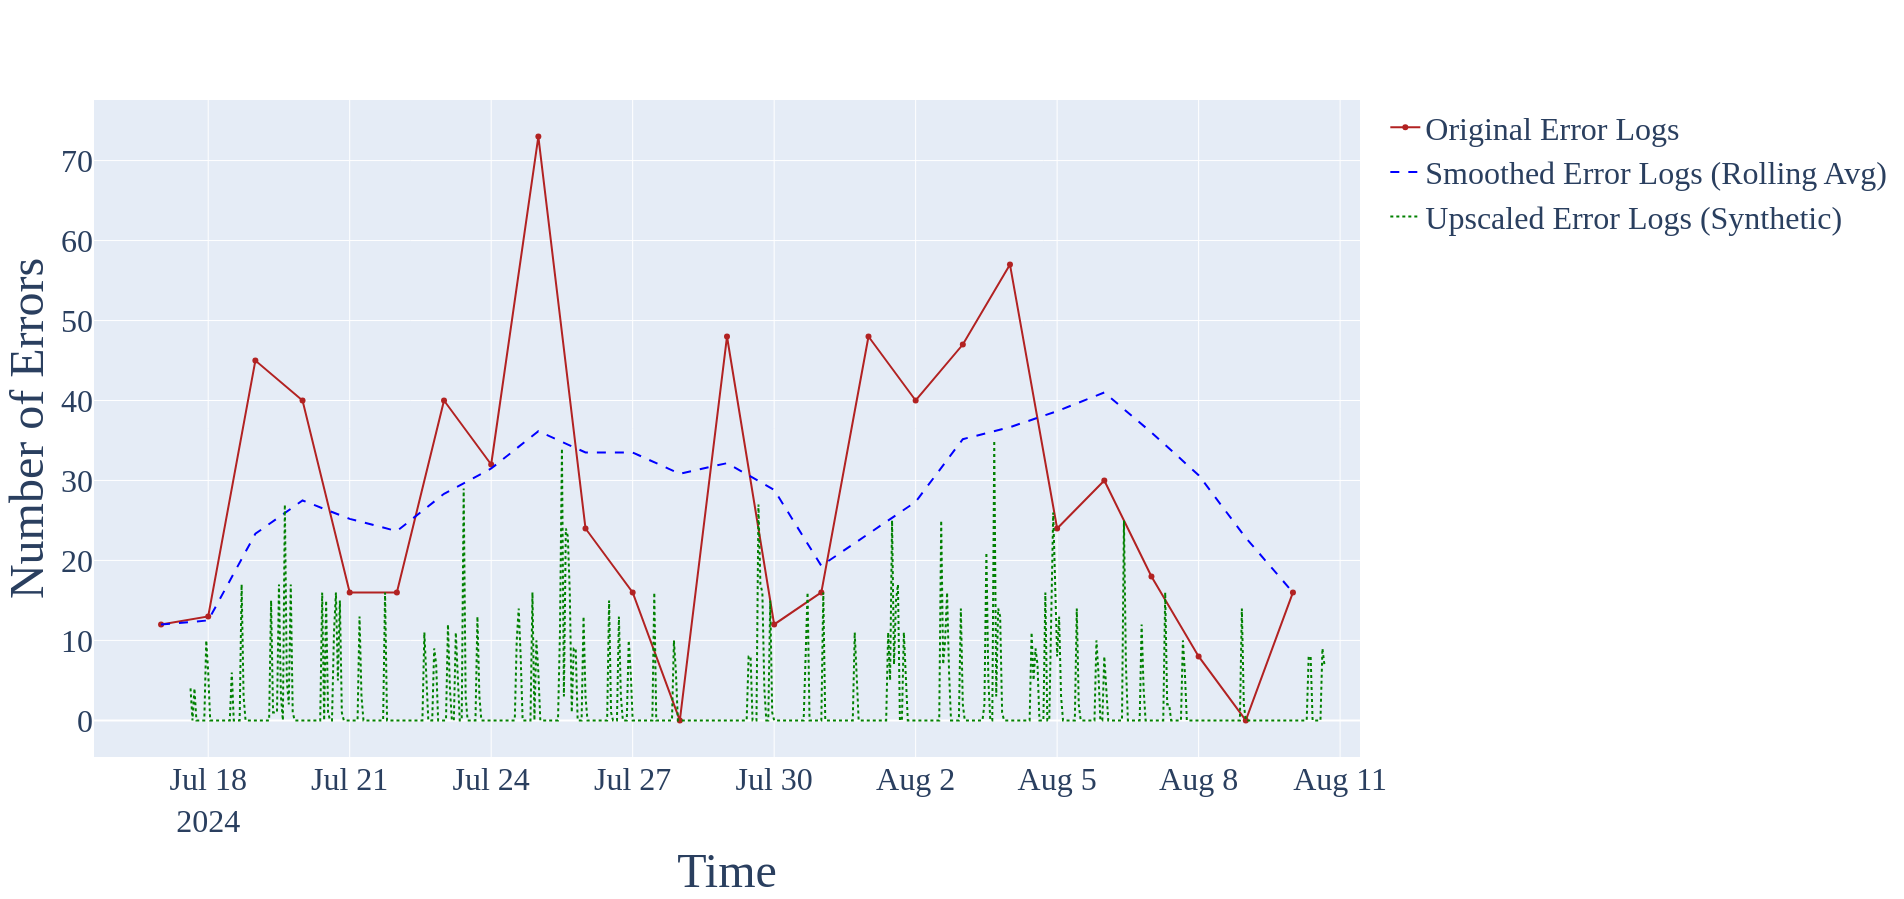
\includegraphics[width=\linewidth]{images/plots/worker/upscaled_error_logs.png}
    \caption[Upscaled Worker Error Logs]{Upscaled Worker Error Logs}\label{fig:worker-upscaled-error-logs}
\end{figure}

\subsection{The Main Cause Behind Worker Errors}

To find out what the main issue behind the Worker errors is, it is again helpful to take a look at the most common error types (see \autoref{fig:worker-error-types}). This shows that more than 90\% of the errors have the error log \textit{"Sending Heartbeat failed"}. A Worker sends a \textit{Heartbeat} HTTP request once per minute to the main \ac{API} with its current status and workload so the \ac{API} has a current overview of all available Workers and can decide which Workers to give tasks to. This error occurs however, when a Worker tries to send such a request and the request fails because the \ac{API} is unreachable. This can either occur because the \ac{API} has become unavailable or because the Worker's \ac{VM} has a network issue. As the main \ac{API} (besides two notable outages that lead to the \ac{API} being offline for a few minutes) had an uptime of 99\%, the error is most likely with the Worker system itself. 
When taking a closer look at the actual logs, especially at other more critical error types that occur less often such as \textit{"Error uploading stream"}, it becomes clear that most of these errors are reported always by the two same Worker \ac{VM}s:

\begin{itemize}
    \item \texttt{labels=\{container=live\_worker..., error=Post "http://vodservice:8089": dial tcp 10.0.1.2:8089: i/o timeout, host=A, level=error, msg=Error\\ uploading stream, stream=..., time=...\}}

    \item \texttt{labels=\{container=live\_worker..., error=Post "http://vodservice:8089": dial tcp 10.0.1.2:8089: i/o timeout, host=B, level=error, msg=Error\\ uploading stream, stream=..., time=...\}}
\end{itemize}

Note that for simplicity, some information has been redacted from the logs and the hosts have been renamed to \texttt{A} and \texttt{B}. However, the main point remains that it appears that the errors occur due to a timeout when trying to reach the VOD Service. As all Workers run on the same Worker-version and on similar \ac{VM}s, and only the two Workers on host \texttt{A} and \texttt{B} report timeout error, it might be due to a misconfiguration or separate issue with the \ac{VM} itself. A possible solution to improve debugging this error would be to include more details of the host \ac{VM} or Worker name in the error log. 

\begin{figure}[htpb]
    \centering
    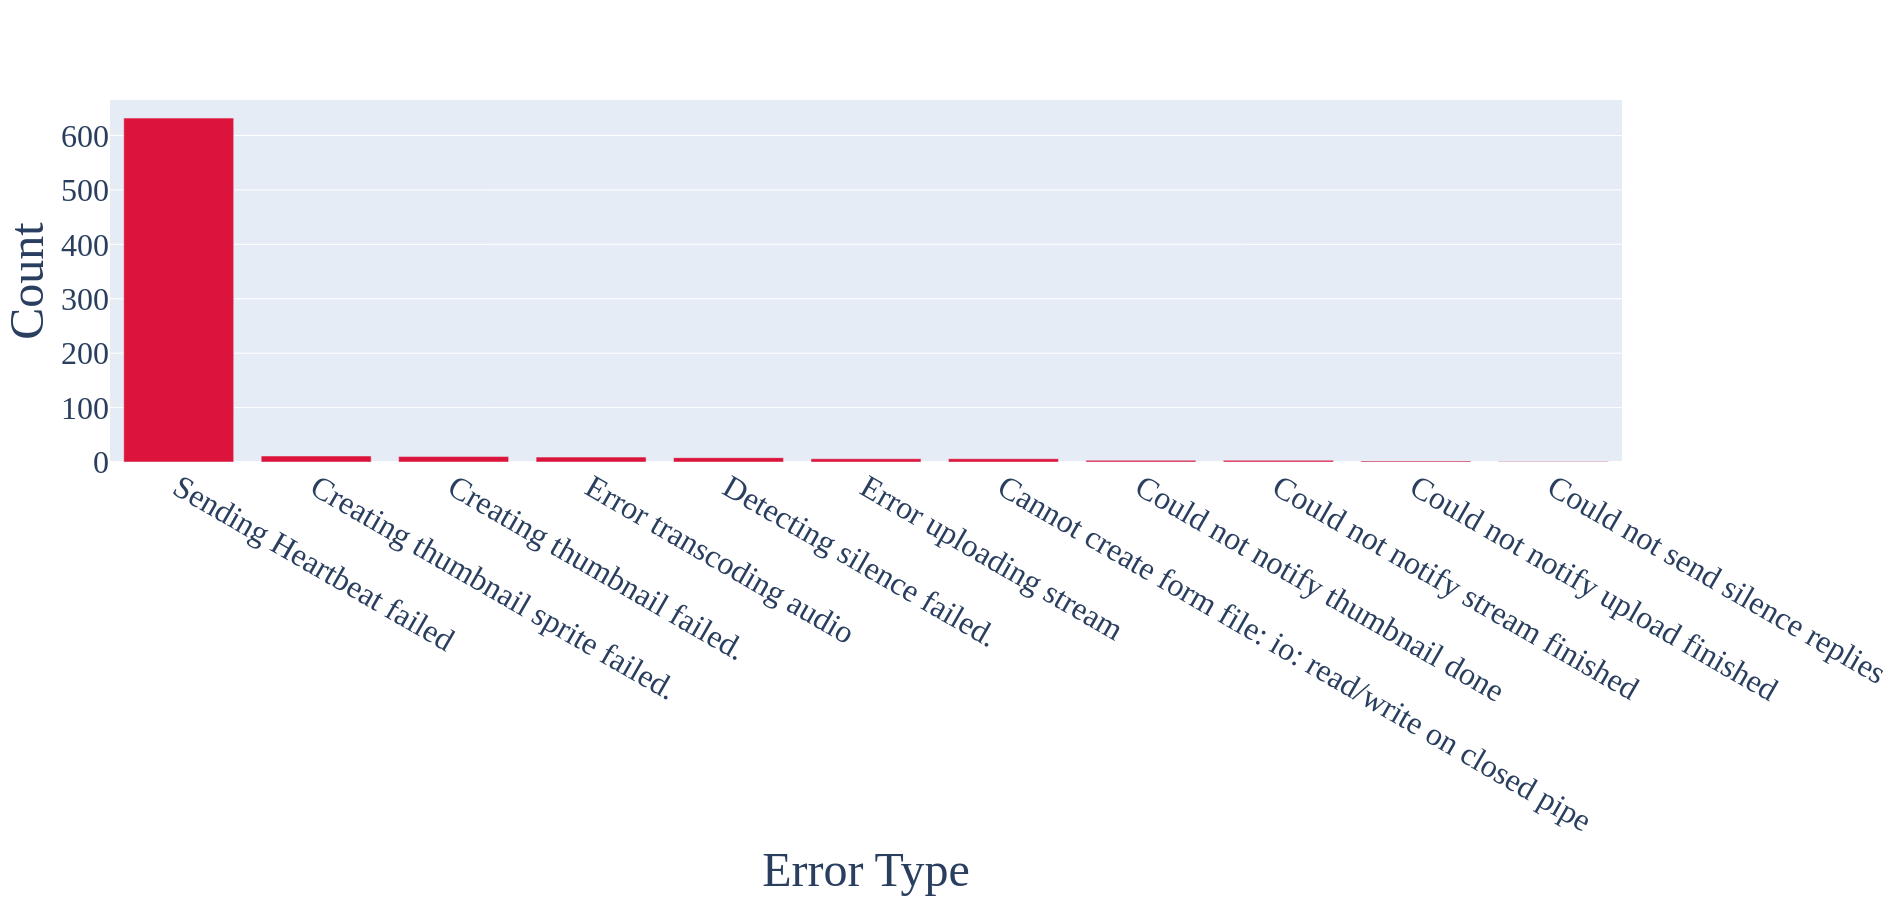
\includegraphics[width=\linewidth]{images/plots/worker/error_types.png}
    \caption[Worker Error Types]{Worker Error Types}\label{fig:worker-error-types}
\end{figure}

\subsection{Future Improvement: Runners}\label{subsection:runner}

At the time of this thesis, GoCast is developing a more robust and scalable alternative to the old Worker system: The Runner. In comparison to the Worker system, which receives a task (e.g., to upload a lecture) and then performs it straightaway, the Runner system works on the basis of queues and jobs. With this, incoming tasks are not just performed resulting in either success or an error, but rather scheduled and handled internally in such a way that a task consists of multiple jobs that can be prioritized accordingly, and, if failed, can be automatically retried multiple times before returning an error. Such a system would most likely solve errors such as the \textit{"Error uploading stream"} error mentioned before as the error would be handled internally and retried within a certain time interval before reporting an error and aborting the task.

% \begin{figure}[htpb]
%     \centering
%     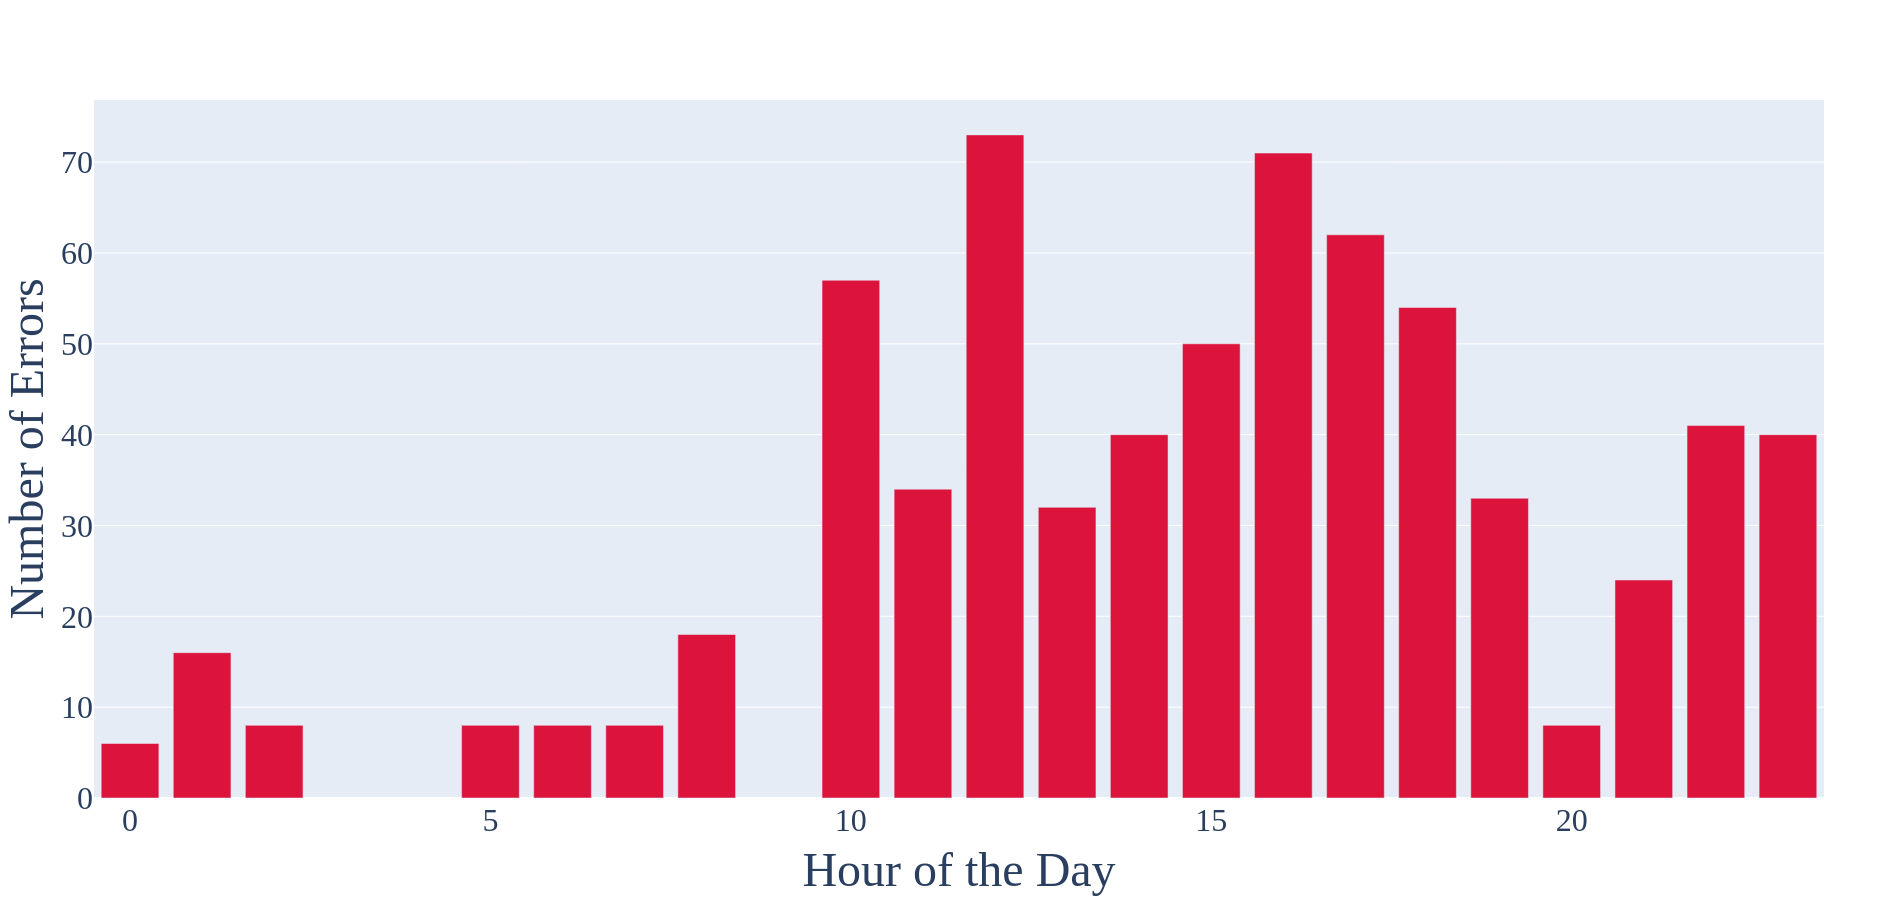
\includegraphics[width=\linewidth]{images/plots/worker/errors_by_hour.png}
%     \caption[Worker Errors by Hour]{Worker Errors by Hour}\label{fig:worker-errors-by-hour}
% \end{figure}

% Based on the collected metrics, the TUM-Live Worker service was identified as a critical bottleneck. As the component responsible for encoding and uploading video streams, it often experiences high CPU and memory loads during peak usage times, leading to potential delays or errors.

% \section{Load Testing Edge Server and VOD Service}
% TODO

\section{A Technical Comparison of REST and gRPC APIs}

While analyzing the performance and limitations of the individual microservices of GoCast can help to resolve bottlenecks, at the core of the entire system there is the main GoCast \ac{API}.
Most services depend on the main \ac{API} to fetch up-to-date information on streams and courses, to send updates on their current status and to notify it whenever there are new streams or \ac{VOD}s. Also, from the end-user's perspective, the \ac{API} needs to handle many concurrent requests as efficiently as possible. Hence, in this section we'll focus on two different \ac{API} design approaches: gRPC and REST.

\subsection{Why gRPC?}

gRPC, released in 2015 by Google, is a modern open-source high performance Remote Procedure Call (RPC) framework that can run cross-platform in any environment. It's strengths are that it can efficiently connect services, supports load balancing, tracing, health checking and authentication.
Another particularity of gRPC is that it automatically generate idiomatic client and server bindings for a service in a variety of languages and platforms using protofiles~\parencite{grpc_vs_rest}.
As it will become clear in the next subsections, it's main advantage over classical HTTP/REST \ac{API}s is that as is based on Protocol Buffers, it has a noticeable stronger performance~\parencite{grpc_vs_rest_2} and supports HTTP/2-based transport and bi-directional streaming, which is difficult with HTTP/1.1, and more efficient than using WebSockets for such purposes~\parencite{grpc_dev}.

\subsection{GoCast's gRPC Prototype and JMeter Test Setup}

GoCast's current REST \ac{API} is written in Go using the \href{https://github.com/gin-gonic/gin}{Gin-Gonic} HTTP web framework. To test if a switch to gRPC would be useful, a prototype for a gRPC \ac{API} V2 was developed and can be found in the \href{https://github.com/carlobortolan/thesis/tree/enh/api\_v2}{enh/api\_v2 branch of github.com/carlobortolan/thesis}.
The prototype is based on the \href{https://google.golang.org/grpc}{official Go gRPC library} and uses \href{https://github.com/protocolbuffers/protobuf}{protoc} used to compile and generate Go code from the \texttt{.proto} files as well as \href{https://github.com/bufbuild/buf}{buf} for managing and generating protobuf files. Currently, only the most important original REST \ac{API} endpoints related to the user, course and stream management are supported by the prototype, as it is mainly intended for test purposes.

\subsubsection{JMeter Configuration and Data Collection}

To perform the performance tests that resulted in the data used in the following section, \href{https://jmeter.apache.org}{Apache JMeter}\footnote{\url{https://jmeter.apache.org}} - an open-source load tester and performance measurer was used. The main advantage of it is, that it exclusively works at protocol level, meaning that it appears and behaves like a browser (or rather, multiple browsers) to web-services, while not performing all the actions supported by browsers. The performed tests were structured using two thread groups - one for REST and one for gRPC - with each having three requests for the respective REST endpoints and gRPC methods:
\begin{itemize}
    \item REST: \texttt{GET:/courses}, \texttt{POST:/user/settings}, \texttt{PATCH:stream/bookmarks}
    \item gRPC: \texttt{getPublicCourses}, \texttt{postSettings}, \texttt{putBookmarks}
\end{itemize}
\break
Each thread group used a thread pool (users) of size 150, a ramp-up period of 10 seconds and a repetition of 10,000 loops.
To measure, compare and export the response time, JMeter-listeners like \textit{Graph Results}, \textit{Summary Report} and \textit{Simple Data Writer} were used. To handle errors and check that the requests were performed successfully, JMeter’s \textit{View Results Tree} was used which captured any failed requests or error codes.

\subsection{Comparison of GoCast's gRPC Prototype and Current REST API}
The tests had a duration of 20 to 30 minutes and performed 1,196,180 HTTP requests with a mean response time of 644.55 ms and 1,171,342 gRPC requests with a mean response time of 162.69 ms. A more detailed overview can be found in \autoref{tab:rest_grpc_statistics}.

\begin{table}[htbp]
\centering
\caption{Statistical Analysis of REST and gRPC Data}
\label{tab:rest_grpc_statistics}
\begin{tabular}{|l|l|l|}
\hline
\textbf{Metric} & \textbf{REST \ac{API}} & \textbf{gRPC \ac{API}} \\ \hline
\textbf{Count} & 1,196,180 & 1,171,342 \\ \hline
\multicolumn{3}{|c|}{\textbf{Elapsed Time}} \\ \hline
Mean & 644.55 ms & 162.69 ms \\ \hline
Standard deviation & 60.38 ms & 36.13 ms \\ \hline
Min & 101 ms & 101 ms \\ \hline
25th percentile & 628 ms & 148 ms \\ \hline
Median (50th percentile) & 642 ms & 152 ms \\ \hline
75th percentile & 659 ms & 175 ms \\ \hline
Max & 4,562 ms & 2,090 ms \\ \hline
\multicolumn{3}{|c|}{\textbf{grpThreads (allThreads for REST)}} \\ \hline
Mean & 149.90 & 149.21 \\ \hline
Standard deviation & 2.94 & 2.28 \\ \hline
Min & 2 & 11 \\ \hline
25th percentile & 150 & 149 \\ \hline
Median (50th percentile) & 150 & 149 \\ \hline
75th percentile & 150 & 150 \\ \hline
Max & 150 & 150 \\ \hline
\end{tabular}
\end{table}

\noindent To evaluate whether gRPC provides significant enough benefits, the focus was on collecting and analyzing the following metrics:

\begin{itemize}
    \item 
        \textbf{Latency}: Response Time of an individual request - see \autoref{fig:comp-distribution}.
        % \begin{figure}[htpb]
        %     \centering
        %         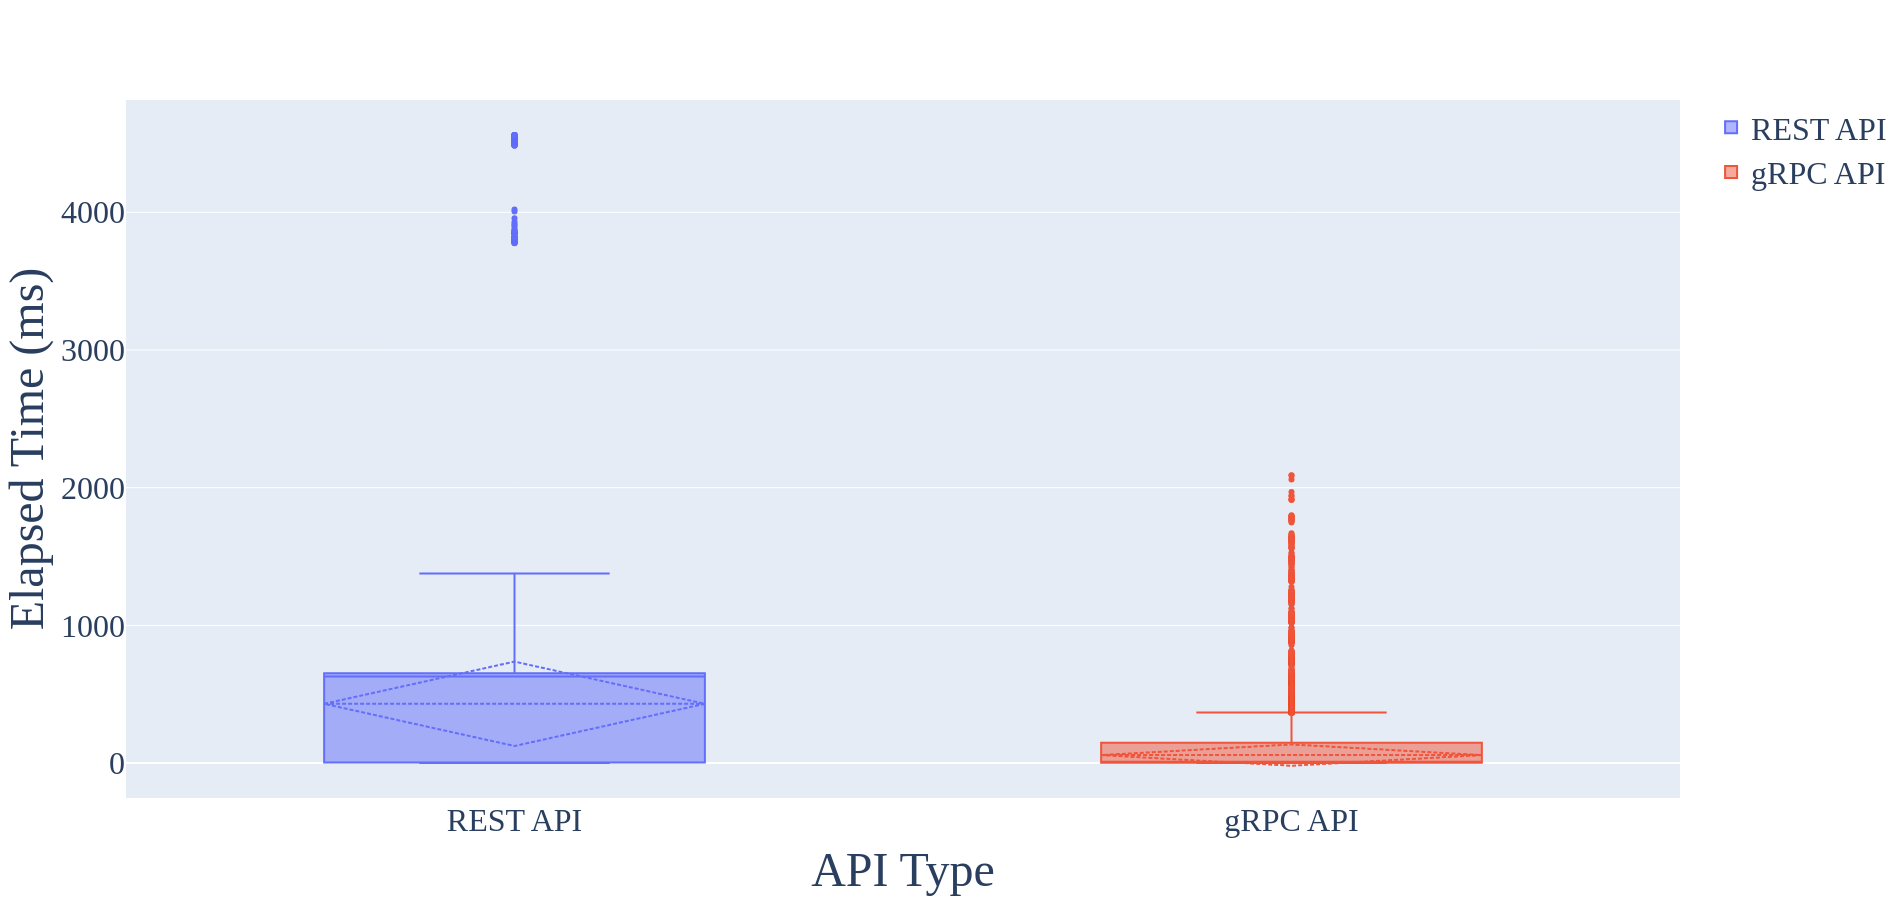
\includegraphics[width=\linewidth]{images/plots/comp/response_time_comparison.png}
        %     \caption[Response Time Comparison]{Response Time Comparison}\label{fig:comp-response-time}
        % \end{figure}
        
        \begin{figure}[htpb]
            \centering
                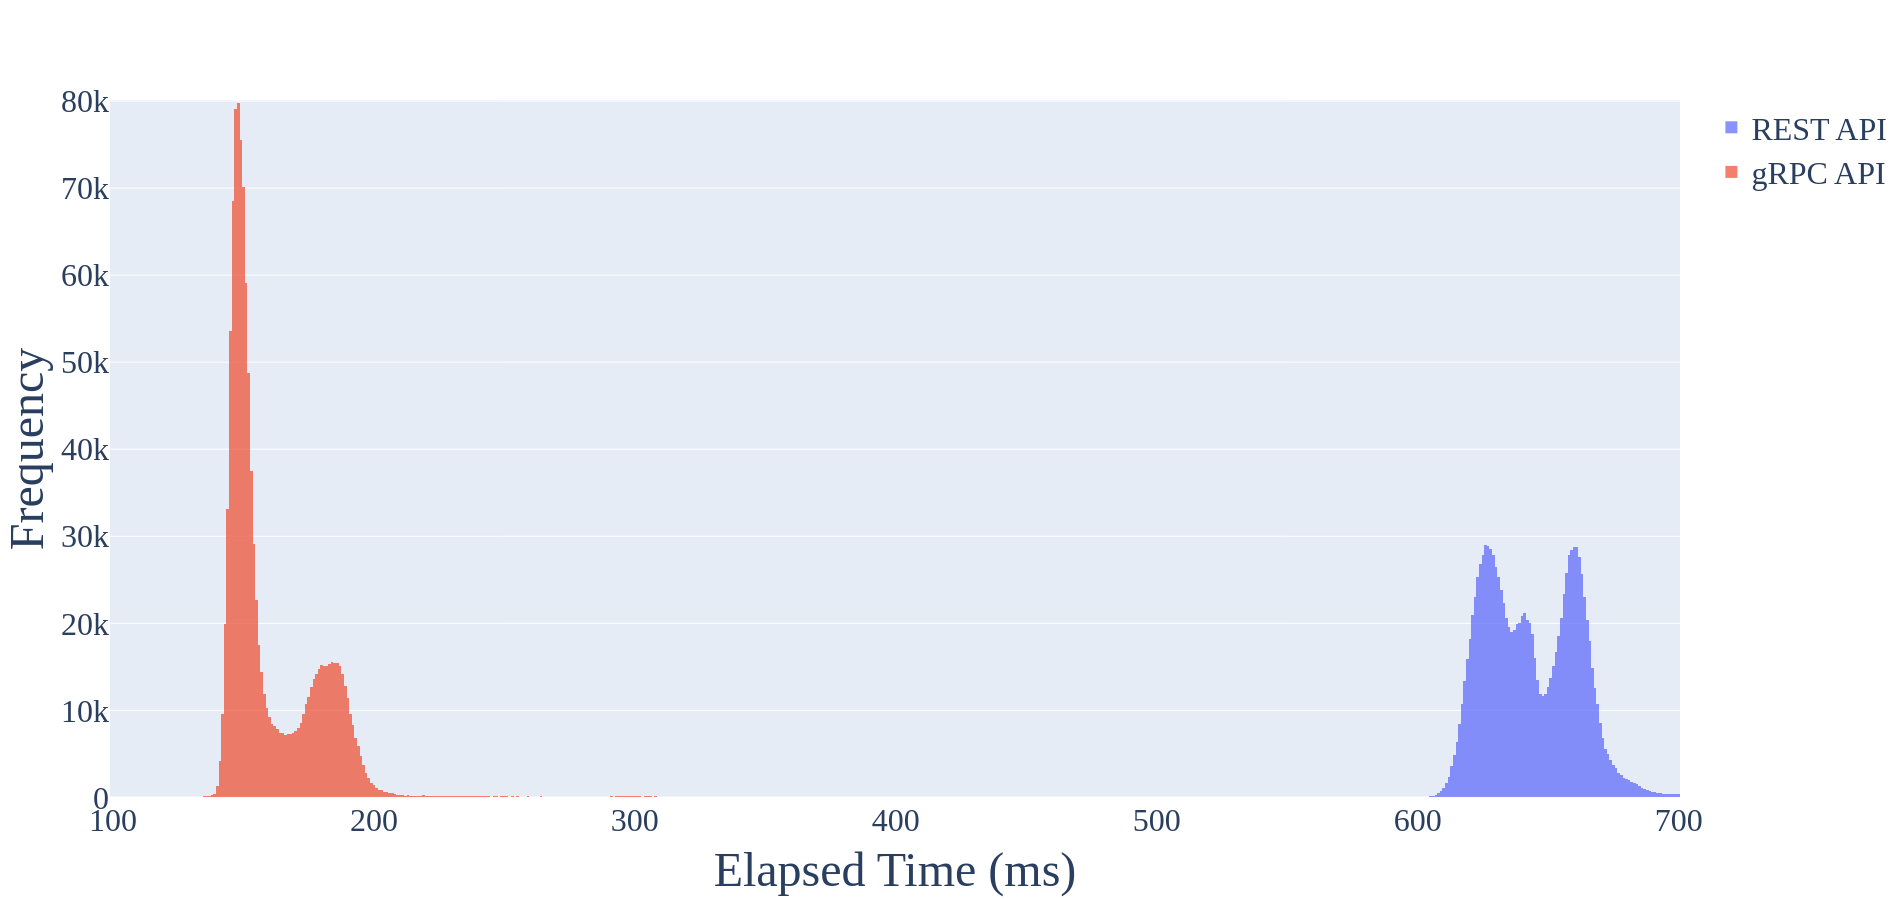
\includegraphics[width=\linewidth]{images/plots/comp/response_time_distribution.png}
            \caption[Response Time Distribution]{Response Time Distribution}\label{fig:comp-distribution}
        \end{figure}
    \item 
        \textbf{Throughput}: How many requests per minutes the \ac{API} can handle - see \autoref{fig:comp-throughput}
        \begin{figure}[htpb]
            \centering
                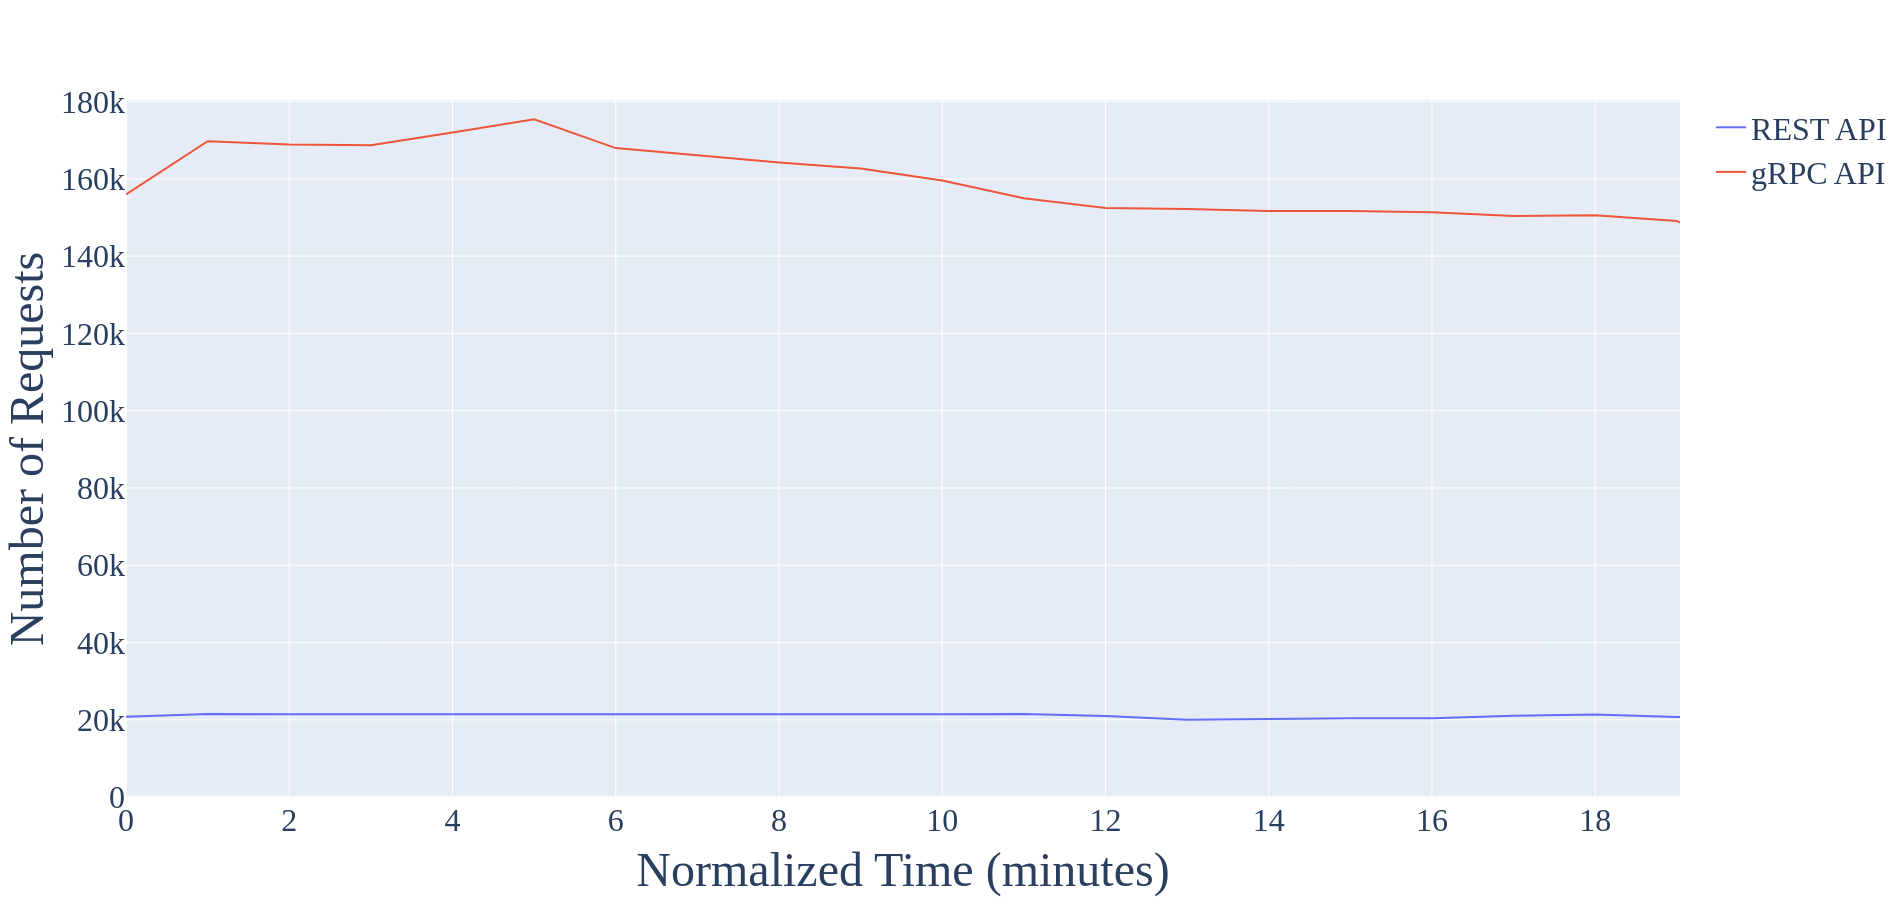
\includegraphics[width=\linewidth]{images/plots/comp/throughput_over_time.png}
            \caption[Throughput over Time]{Throughput over Time}\label{fig:comp-throughput}
        \end{figure}
\end{itemize}

\subsection{Results}

As expected, gRPC is significantly faster due to its use of Protocol Buffers and HTTP/2, which reduces overhead compared to HTTP/1.1. To evaluate whether gRPC justifies the effort of switching the \ac{API} Design, there are three main considerations:

\begin{enumerate}
    \item \textbf{Performance Benefits}: gRPC offers approximately a 3-times significant reduction in latency and an 8 times increase in throughput. It can also be observed in \autoref{fig:comp-response-time} that the standard deviation of the response time with gRPC requests (36.13 ms) is nearly half that of HTTP requests (60.38 ms) which could lead to an overall more stable \ac{API} performance.  When considering outliers, the gRPC \ac{API} again outperforms the REST \ac{API}, having a maximum latency of 2,090 ms for slow requests compared to 4,562 ms for the REST \ac{API}.

    \item \textbf{Browser Compatibility}: While the lack of native browser support for gRPC might make REST a better fit, the current gRPC prototype exposes a HTTP Gateway that can be accessed just like a REST \ac{API} by browser-based clients. Also, the gRPC prototype only contained "normal" endpoints, but considering the many real-time use cases that come with streaming (e.g., the live chat), gRPC’s bidirectional streaming could be a big advantage over REST.

    \item \textbf{Migration Effort}: Migrating to gRPC would require a complete re-implementation from scratch of the GoCast \ac{API} with significant changes to the clients and infrastructure. While tools for REST are widely spread (e.g., Postman, cURL), the gRPC ecosystem currently has fewer options for debugging, monitoring, and testing and often requires installing additional third-party add-ons to make commonly used tools compatible with gRPC.
\end{enumerate}

\section{Limitations of the Current System}

Given the analyzed data and review of GoCast's codebase, some limitations have been found that could become major issues when scaling up the current system.

\subsection{GoCast's In-Memory Chat System}

A major limitation of GoCast is its chat system. Currently, it is implemented as a combination of TCP and WebSockets to transmit real-time updates to viewers, but saves the actual chat channels in memory. This means that if the main \ac{API} would be scaled to multiple instances and two users were to connect to two separate instances, their chat messages would never reach the other instance. A possible solution for this problem would be to refactor the chat system on the server-side to store the chat messages in a separate in-memory database such as \href{https://redis.io}{Redis}\footnote{\url{https://redis.io}} or use distributed messaging services such as \href{https://github.com/nats-io/nats-server}{NATS.io}\footnote{\url{https://github.com/nats-io/nats-server}}. Alternatively, it is also possible to fix this issue by always having a certain GoCast instance being responsible for a certain chat or defining a hash function that determines to which instance messages of a certain stream should be posted.

\subsection{N+1 Queries}

Another weakness of the current system is the N+1 query problem, which is the result of multiple database queries executed to fetch data between \ac{ORM} models. The N+1 query problem occurs when one initial query is followed by N additional queries for associated data, leading to performance degradation when N is large. In the current implementation, certain database operations, especially when retrieving courses and their associated streams or users, have this issue, as instead of creating one longer query that returns the given object and associations, first one query retrieves the object itself and then N queries retrieve the associated objects individually. This results in a high number of queries being executed (N+1 instead of only 1) and negatively impacts performance, especially at scale.

\subsubsection{Example of N+1 Problem in the Current Code:}

In the \texttt{liveStreams} method, for each live stream retrieved by the \texttt{GetCurrentLive} query, additional queries are executed to fetch the associated course and lecture hall.

\begin{figure}[htpb]
  \begin{tabular}{c}
  \ \small \begin{lstlisting}[language=Go]
    // returns all streams that are live
    func (r streamRoutes) liveStreams(c *gin.Context) {
        streams, err := r.StreamsDao.GetCurrentLive(c)
        // ...
        for _, s := range streams {
            course, err := r.CoursesDao.GetCourseById(c, s.CourseID)
            lectureHall, err := r.LectureHallsDao.GetLectureHallByID(s.LectureHallID)
            // ...
    \end{lstlisting}
  \end{tabular}
  \label{fig:n+1-example-livestreams}
\end{figure}

\begin{enumerate}
    \item The first query retrieves all currently live streams.
    \item For each stream, a separate query fetches its associated course.
    \item For each stream, an additional query fetches its associated lecture hall.
\end{enumerate}

\noindent This leads to N additional queries for the courses and lecture halls for each live stream, resulting in a total of 2N queries plus one initial query for fetching the streams. As we know from \autoref{subsection:user-stats-tumlive}, TUM-Live can have up to 100 active streams with more than 1,000 viewers a day, resulting in a significant number of unnecessary queries.

\subsubsection{Possible Solutions:}

\begin{enumerate}

\item \textbf{Use Preloading to Eagerly Load Associations}: By preloading the associated data (courses and lecture halls) in a single query, the number of database queries can be reduced to a minimum. For example, the \texttt{GetCurrentLive} method could be refactored to preload the \texttt{Course} and \texttt{LectureHall} fields as shown below:

    \begin{figure}[htpb]
      \begin{tabular}{c}
      \ \small \begin{lstlisting}[language=Go]
        func (d *StreamsDao) GetCurrentLive(ctx context.Context) ([]model.Stream, error) {
            var streams []model.Stream
            err := DB.Preload("Course") // eagerly load stream's course
                     .Preload("LectureHall") // eagerly load stream's lecturehalls
                     .Where("live_now = ?", true)
                     .Find(&streams).Error
            return streams, err
        }
      \end{lstlisting}
      \end{tabular}
    \end{figure}

Now, the \texttt{liveStreams} endpoint does not need to making additional queries for each stream:
    
    \begin{figure}[htpb]
      \begin{tabular}{c}
      \ \small \begin{lstlisting}[language=Go]
        func (r streamRoutes) liveStreams(c *gin.Context) {
            streams, err := r.StreamsDao.GetCurrentLive(c)
            // ...
            for _, s := range streams {
                lectureHall = s.LectureHall
                course = s.course
                // ...
            }
        }
      \end{lstlisting}
      \end{tabular}
    \end{figure}

    \item \textbf{Batch Queries}: Instead of loading each object one by one, the \texttt{GetCurrentLive} method could collect the IDs of currently live stream first and then batch the queries, reducing the number of database calls.

    \item \textbf{Caching}: While not particularly fitting for this example, N+1 queries can be resolved by caching frequently accessed data (with careful invalidation) to reduce overall database queries.

    \item \textbf{GraphQL or DataLoader}: A more advanced solution would be to use batching mechanisms like \href{https://github.com/graphql/dataloader}{DataLoader}\footnote{\url{https://github.com/graphql/dataloader}}, often used in GraphQL environments, to batch multiple requests for related data into a single query.
\end{enumerate}


\subsection{Other Factors for API Design}

While the gRPC prototype showed promising results, when it comes to comparing the different \ac{API} design approaches, there are additional factors that can be considered:

\begin{itemize}
    \item \textbf{Resource Usage (CPU, Memory, Network)}
    It might be interesting to compare how efficiently each \ac{API} handles resources under load. gRPC, with its smaller binary payloads, may consume less bandwidth, but may use more CPU. 
    Also, for potential bandwidth issues, network traffic could be analyzed to understand the differences in payload size and bandwidth usage.
    
    \item \textbf{Error Rates and Reliability}
    In a production-like environment for testing purposes it could be evaluated how both systems behave under load or failure scenarios. Does one \ac{API} lead to more errors under heavy load, or can both handle the same level of traffic? One could measure the error rate (=percentage of failed requests during the test) or the time to recover from errors or failures (e.g., retries, handling errors, etc.).
\end{itemize}

% !TeX root = ../main.tex
% !TeX root = ../main.tex
% Add the above to each chapter to make compiling the PDF easier in some editors.

\chapter{Outlook}\label{chapter:outlook}

Specialized Clouds for Video Streaming (?)

Single Streaming Engine for both Live- and VOD-Streaming (?)

Blockchain Technology for Video Streaming (?)

Machine Learning for Video Processing (?)

Media Over QUIC (?)
% !TeX root = ../main.tex
% !TeX root = ../main.tex
% Add the above to each chapter to make compiling the PDF easier in some editors.

\chapter{Conclusion}\label{chapter:conclusion}

Video streaming infrastructure is a fascinating topic often taken for granted by users who open Netflix or YouTube and start streaming videos for hours without an idea of the complexity of what happens behind the screen when they press the "play" button. This thesis has not only shown how enterprise-grade streaming architecture is built and optimized to its limit, but also demonstrated the hands-on process of scaling TUM-Live. Besides scaling it to a distributed system that allows organizations to share computing resources and storage, microservices like the RTMP-Proxy now made features such as self-streaming more accessible. With this, TUM-Live will be able to be used not just by the \ac{CIT}, but also by other \ac{TUM} schools and universities.
Additionally, we have found that there are still areas with room for improvement, including performance bottlenecks, complicated error management, N+1 queries and the issue of having an in-memory chat. Lastly, this thesis also provided concrete solutions and optimizations, such as the \ac{gRPC} \ac{API} that reduced latency by 3x and improved throughput by 8x compared to the current system. 

Hopefully this thesis will serve as a useful resource for developers working on the GoCast architecture, researches exploring new streaming technologies, professionals looking for alternative scaling solutions and all individuals interested in understanding what really happens when they press "play".

% TODO: add more chapters here

\appendix{}

\microtypesetup{protrusion=false}

\addchap{Abbreviations}
\begin{acronym}
	\itemsep-.25\baselineskip
	% TODO: add acronyms
	\acro{TUM}[TUM]{Technical University of Munich}
	\acro{LRZ}[LRZ]{Leibniz Supercomputing Centre}
	\acro{SMP}[SMP]{Streaming Media Processor}
	\acro{VMP}[VMP]{Virtual Media Processor}
	\acro{CIT}[CIT]{School of Computation, Information and Technology}
 	\acro{VM}[VM]{Virtual Machine}
 	\acro{DB}[DB]{Database}
 	\acro{SMP}[SMP]{Streaming Media Processors}
 	\acro{VMP}[VMP]{Virtual Media Processor}
 	\acro{ITO}[ITO]{IT Operations}
 	\acro{SSO}[SSO]{Single Sign On}
 	\acro{LDAP}[LDAP]{Lightweight Directory Access Protocol}
 	\acro{SAML}[SAML]{Security Assertion Markup Language}
 	\acro{API}[API]{Application Programming Interface}
 	\acro{AWS}[AWS]{Amazon Web Services}
 	\acro{EKS}[EKS]{Elastic Kubernetes Service}
 	\acro{CDN}[CDN]{Content Delivery Network}
 	\acro{ISPs}[ISPs]{Internet Service Providers}
 	\acro{HLS}[HLS]{HTTP Live Streaming}
 	\acro{RTMP}[RTMP]{Real-Time Messaging Protocol}
 	\acro{POPs}[POPs]{Points of Presence}
 	\acro{VOD}[VOD]{Video on Demand}
 	\acro{IRC}[IRC]{Internet Relay Chat}
 	\acro{QA}[QA]{Quality Assurance}
 	\acro{P2P}[P2P]{Peer-to-Peer}
 	\acro{ABR}[ABR]{Adaptive Bitrate Transcoding}
 	\acro{AES}[AES]{Advanced Encryption Standard}
 	\acro{JWT}[JWT]{JSON Web Token}
 	\acro{TLS}[TLS]{Transport Layer Security}
 	\acro{DRM}[DRM]{Digital Rights Management}
 	\acro{ACID}[ACID]{Atomicity, Consistency, Isolation, Durability}
 	\acro{LP}[LP]{Linear Program}
 	\acro{OCAs}[OCAs]{Open Connect Appliances}
    \acro{ORM}[ORM]{Object-relational mapper}
 	\acro{MBone}[MBone]{Multicast Backbone}
    \acro{VCU}[VCU]{Video Coding Unit}
\end{acronym}

\listoffigures{}
\listoftables{}
\microtypesetup{protrusion=true}
\printbibliography{}

\end{document}
